%%%%%%%%%%%%%%%%%%%%%%%%%%%%%%%%%%%%%%%%%
% Thesis 
% LaTeX Template
% Version 1.3 (21/12/12)
%
% This template has been downloaded from:
% http://www.latextemplates.com
%
% Original authors:
% Steven Gunn s
% http://users.ecs.soton.ac.uk/srg/softwaretools/document/templates/https://preview.overleaf.com/phttps://preview.overleaf.com/public/qmpmgrsjhbjk/images/988840e05aa9bab85df8b9f50121f4f02ad9e8c1.jpegublic/qmpmgrsjhbjk/images/988840e05aa9bab85df8b9f50121f4f02ad9e8c1.jpeg
% and
% Sunil Patel
% http://www.sunilpatel.co.uk/thesis-template/
%
% License:
% CC BY-NC-SA 3.0 (http://creativecommons.org/licenses/by-nc-sa/3.0/)
%
% Note:
% Make sure to edit document variables in the Thesis.cls file
%
%%%%%%%%%%%%%%%%%%%%%%%%%%%%%%%%%%%%%%%%%

%----------------------------------------------------------------------------------------
%	PACKAGES AND OTHER DOCUMENT CONFIGURATIONS
%----------------------------------------------------------------------------------------

\documentclass[11pt, a4paper, oneside]{thesis} % Paper size, default font size and one-sided paper

%extras
\usepackage{afterpage}
\usepackage{booktabs}
\usepackage{amsmath}
\usepackage{verbatim}
\usepackage{epigraph}
\usepackage{float}
\usepackage{tikz}
\usepackage{gantt}
\usepackage{multirow}
\usepackage{rotating,graphics}
\usepackage{tabu}
\usepackage{listings}
\usepackage{xcolor}
\usepackage{amssymb}% http://ctan.org/pkg/amssymb
\usepackage{pifont}% http://ctan.org/pkg/pifont
\newcommand{\cmark}{\ding{51}}%
\newcommand{\xmark}{\ding{55}}%
\usepackage{slashbox}
\usepackage{lscape}
\usepackage{pdflscape}
\usepackage{amsmath}
\usepackage{algorithm}
\usepackage{caption}
\usepackage{pbox}
\usepackage{adjustbox}
\usepackage{algorithm}
\usepackage[noend]{algpseudocode}
\urlstyle{same} 

\usepackage{xcolor,colortbl}
\definecolor{green}{rgb}{0,1,0}
\definecolor{red}{rgb}{1,0,0}

\newcommand{\ccheck}{\cellcolor{green}\cmark}  %{0.9}
\newcommand{\xcheck}{\cellcolor{red}\xmark}

\newcommand{\norm}[1]{\left\lVert#1\right\rVert}

\newcommand\blankpage{%
    \null
    \thispagestyle{empty}%
    \addtocounter{page}{-1}%
    \newpage}

\colorlet{punct}{red!60!black}
\definecolor{background}{HTML}{EEEEEE}
\definecolor{delim}{RGB}{20,105,176}
\colorlet{numb}{magenta!60!black}

\taburulecolor{black}



\graphicspath{{./Pictures/}} % Specifies the directory where pictures are stored

\usepackage[square, comma,sort&compress]{natbib} % Use the natbib reference package - read up on this to edit the reference style; if you want text (e.g. Smith et al., 2012) for the in-text references (instead of numbers), remove 'numbers' 
\hypersetup{urlcolor=blue, colorlinks=false} % Colors hyperlinks in blue - %change to black if annoying
\title{\ttitle} % Defines the thesis title - don't touch this

%PREAMBLE
\usepackage[intoc]{nomencl}
\renewcommand{\nomname}{Nomenclature}
\setlength{\nomitemsep}{-\parsep}
\makenomenclature

\nomenclature{\ensuremath{\textbf{P}}}{Precision}
\nomenclature{\ensuremath{\textbf{R}}}{Recall}
\nomenclature{\ensuremath{\textbf{F}_\textbf{1}}}{F-measure considering Harmonic Mean of Recall and Precision}
\nomenclature{\ensuremath{\textbf{P$\mu$}}}{Micro Precision}
\nomenclature{\ensuremath{\textbf{P$^{M}$}}}{Macro Precision}
\nomenclature{\ensuremath{\textbf{R$\mu$}}}{Micro Recall}
\nomenclature{\ensuremath{\textbf{R$^{M}$}}}{Macro Recall}

\begin{document}

\frontmatter % Use roman page numbering style (i, ii, iii, iv...) for the pre-content pages

\setstretch{1.3} % Line spacing of 1.3

% Define the page headers using the FancyHdr package and set up for one-sided printing
\fancyhead{} % Clears all page headers and footers
\rhead{\thepage} % Sets the right side header to show the page number
\lhead{} % Clears the left side page header

\pagestyle{fancy} % Finally, use the "fancy" page style to implement the FancyHdr headers

\newcommand{\HRule}{\rule{\linewidth}{0.5mm}} % New command to make the lines in the title page



% PDF meta-data
\hypersetup{pdftitle={\ttitle}}
\hypersetup{pdfsubject=\subjectname}
\hypersetup{pdfauthor=\authornames}
\hypersetup{pdfkeywords=\keywordnames}

%----------------------------------------------------------------------------------------
%	COVER PAGE
%----------------------------------------------------------------------------------------
\begin{titlepage}
\begin{center}

\textsc{\LARGE \univname}\\[1.5cm] % University name
%\textsc{\Large Dissertation/Final Report}\\[0.5cm] % Thesis type
\textsc{\Large Dissertation}\\[0.5cm] % Thesis type
\textsc{}\\[0.5cm] % Thesis type

\HRule \\[0.4cm] % Horizontal line
{\huge \bfseries \ttitle}\\[0.4cm] % Thesis title
\HRule \\[1.5cm] % Horizontal line
 
\begin{minipage}{0.4\textwidth}
\begin{flushleft} \large
\emph{Author:}\\
\authornames % Author name - remove the \href bracket to remove the link
\end{flushleft}
\end{minipage}
\begin{minipage}{0.5\textwidth}
\begin{flushright} \large
\emph{Advisors:} \\
\supname % Supervisor name - remove the \href bracket to remove the link  
\end{flushright}
\end{minipage}\\[3cm]
 
\large \textit{Thesis submitted in partial fulfillment of the requirements\\ for the degree of \degreename}\\[0.3cm] % University requirement text

\facname\\\deptname\\[2cm] % Faculty name and department name
 
{\large September, 2016}\\[2cm] % Date

\includegraphics[height=24mm]{Figures/MARCA_UC_LET_PRETO} 
\vfill
\end{center}

\end{titlepage}
\afterpage{\blankpage}
\clearpage % Start a new page
%----------------------------------------------------------------------------------------
%	BACK PAGE
%----------------------------------------------------------------------------------------
\begin{titlepage}
\begin{center}

\textsc{\LARGE \univname}\\[1.5cm] % University name
%\textsc{\Large Dissertation/Final Report}\\[0.5cm] % Thesis type
\textsc{\Large Dissertation}\\[0.5cm] % Thesis type
\textsc{}\\[0.5cm] % Thesis type

\HRule \\[0.4cm] % Horizontal line
{\huge \bfseries \ttitle}\\[0.4cm] % Thesis title
\HRule \\[1.5cm] % Horizontal line
 
\begin{minipage}{0.4\textwidth}
\begin{flushleft} \large
\emph{Author:}\\
\authornames % Author name - remove the \href bracket to remove the link
\end{flushleft}
\end{minipage}
\begin{minipage}{0.5\textwidth}
\begin{flushright} \large
\emph{Advisors:} \\
\supname % Supervisor name - remove the \href bracket to remove the link  
\end{flushright}
\end{minipage}\\[0.5cm]

\begin{minipage}{0.90\textwidth}
\begin{flushright} \large
\emph{Jury:} \\
Prof. Dr. Bernardete Ribeiro \\ Prof. Dr. Bruno Cabral 
\end{flushright}
\end{minipage}\\[1cm]
 
\large \textit{Thesis submitted in partial fulfillment of the requirements\\ for the degree of \degreename}\\[0.3cm] % University requirement text

\facname\\\deptname\\[2cm] % Faculty name and department name
 
{\large September, 2016}\\[2cm] % Date

\includegraphics[height=24mm]{Figures/MARCA_UC_LET_PRETO} 
\vfill
\end{center}

\end{titlepage}
\afterpage{\blankpage}
\clearpage % Start a new page

%----------------------------------------------------------------------------------------
%	QUOTATION PAGE
%----------------------------------------------------------------------------------------


\pagestyle{empty} % No headers or footers for the following pages


%\null\vfill % Add some space to move the quote down the page a bit
%\vspace{40cm}
%\topskip0pt
\vspace*{\fill}
\begin{center}
\textit{To Rui, Ana and Adolfo.}
\end{center}
\vspace*{\fill}


\afterpage{\blankpage}
\clearpage % Start a new page


%\vfill\vfill\vfill\vfill\vfill\vfill\null % Add some space at the bottom to position the quote just right

%\clearpage % Start a new page

\acknowledgements{\addtocontents{toc}{\vspace{1em}} % Add a gap in the Contents, for aesthetics

I would like to thank my advisers, Prof. Hugo Gonçalo Oliveira and Prof. Ana Oliveira Alves for all their guidance, support and helpful advice. I would also like to thank the rest of the research team that was part of this project for their contributions.\\
I am grateful to my family, friends and anybody who somehow contributed and helped me get where I am now.
}
\afterpage{\blankpage}
\clearpage % Start a new page

%----------------------------------------------------------------------------------------
%	ABSTRACT PAGE
%----------------------------------------------------------------------------------------

\addtotoc{Abstract} % Add the "Abstract" page entry to the Contents

\thispagestyle{empty}
 %% \null\vfil
  \begin{center}
    \setlength{\parskip}{0pt}
    {\huge{\textit{Abstract}} \par}
    \bigskip
  \end{center}

Given the overwhelming quantity of messages posted in social networks, in order to to make their utilization more productive, it is imperative to filter out irrelevant information. 
This work is focused on the automatic classification of public social data according to its potential \textit{relevance} to a general audience, according to journalistic criteria. This means filtering out information that is private, personal, not important or simply irrelevant to the public, improving the the overall quality of the social media information.\\
A range of natural language processing toolkits was first assessed while performing a set of standard tasks in popular datasets that cover newspaper and social network text. After that, different learning models were tested, using linguistic features extracted by some of the previous toolkits. The prediction of journalistic criteria,  key in the assessment of relevance, was also explored, using the same features. A new classifier uses the journalist predictions, made by an ensemble of linguistic classifiers, as features to detect relevance. The obtained model achieved a F$_1$ score of 0.82 with an area under the curve(AUC) equal to 0.78. 

% The Web is a social creation. People use it to communicate and share ideas. Social networks are specially tailored for this kind of activities since people use them to ask questions, share observations and engage in meaningful discussions and are usually a faster way to receive news than traditional media like newspapers, magazines, etc. Thus, social networks are a great source of information and social data. Mining the social web offers a large number of possibilities including providing intelligent recommendations. This dissertation involves the development of a system that classifies public social data according to its potential \textit{relevance} to a general audience. This means filtering out information that is private, personal, not important or simply irrelevant to the public. Our methodology will be based on a standard machine learning approach where the set of features of our model will be extracted through common Natural Language Processing tasks. The end result will be a model of \textit{relevance} which makes automatic \textit{relevance} predictions.

%This dissertation involves the development of a system that classifies public social data according to its potential \textit{relevance} to a general audience. This means filtering out information that is private, personal, not important or simply irrelevant to the public. Our methodology will be based on a standard supervised machine learning approach where the set of features of our model will be extracted through common Natural Language Processing tasks. The end result will be a model of \textit{relevance} which makes automatic \textit{relevance} predictions. Current work includes a review of the literature, from both scientific and technological perspectives, experimentation with standard NLP tools, in order to assess their performance on different kinds of texts, namely social and formal text, and an initial classification experiment with a machine learning toolkit.

\textbf{Keywords: } \keywordnames Relevance Assessment, Social Mining, Information Extraction, Natural Language Processing, Automatic Text Classification 

\afterpage{\blankpage}
\clearpage % Start a new page

\thispagestyle{empty}
 %% \null\vfil
  \begin{center}
    \setlength{\parskip}{0pt}
    {\huge{\textit{Resumo}} \par}
    \bigskip
  \end{center}

%\abstract{\addtocontents{toc}{\vspace{1em}} % Add a gap in the Contents, for aesthetics

Dada a grande quantidade de dados publicada em redes sociais, é imperativo filtrar informação irrelevante. Este trabalho foca-se na detecção automática de dados sociais públicos de acordo com a sua relevância para a audiência em geral. Isto significa filtrar informação que é privada, pessoal, não importante, ou simplesmente irrelevante para o público, melhorando assim a qualidade da informação. \\
Um conjunto de ferramentas de linguagem em processamento natural é testado em uma série de tarefas padrão com um conjunto de dados que cobrem conteúdo jornalístico e texto social. Para além disso, diferentes modelos de aprendizagem são testados, usando características linguísticas extraídas através de tarefas de processamento de linguagem natural, bem como critérios jornalísticos. O sistema final usa as previsões jornalísticas, realizadas por um conjunto de classificadores linguísticos, como atributos para detectar relevância. O modelo obtido alcançou um valor de F$_1$ de 0.82 com uma área debaixo da curva(AUC) igual a 0.78.  

\textbf{Palavras chave: } \keywordnames Detecção de Relevância, Extracção de Dados Sociais, Extracção de Conhecimento, Processamento de Linguagem Natural, Classificação Automática de Texto 


\afterpage{\blankpage}
\clearpage % Start a new page
%----------------------------------------------------------------------------------------
%	ACKNOWLEDGEMENTS
%----------------------------------------------------------------------------------------


\setstretch{1.3} % Reset the line-spacing to 1.3 for body text (if it has changed)



%----------------------------------------------------------------------------------------
%	LIST OF CONTENTS/FIGURES/TABLES PAGES
%----------------------------------------------------------------------------------------

\pagestyle{fancy} % The page style headers have been "empty" all this time, now use the "fancy" headers as defined before to bring them back

\lhead{\emph{Contents}} % Set the left side page header to "Contents"
\tableofcontents % Write out the Table of Contents

\lhead{\emph{List of Figures}} % Set the left side page header to "List of Figures"
\listoffigures % Write out the List of Figures

\lhead{\emph{List of Tables}} % Set the left side page header to "List of Tables"
\listoftables % Write out the List of Tables


%\lhead{\emph{List of Algorithms}}
%\listofalgorithms



%----------------------------------------------------------------------------------------
%	ABBREVIATIONS
%----------------------------------------------------------------------------------------


\clearpage % Start a new page

\setstretch{1.5} % Set the line spacing to 1.5, this makes the following tables easier to read

\lhead{\emph{Acronyms}} % Set the left side page header to "Abbreviations"
\renewcommand*\listsymbolname{Acronyms}

% \listofsymbols{ll} % Include a list of Abbreviations (a table of two columns)
% {


% \textbf{CoNLL} & \textbf{C}onference on \textbf{N}atural \textbf{L}anguage \textbf{L}earning \\
% \textbf{TREC} & \textbf{T}ext \textbf{RE}trieval \textbf{C}onference \\
% \textbf{LDC} & \textbf{L}inguistic \textbf{D}ata \textbf{C}onsortium \\
% \textbf{CCG} & \textbf{C}ognitive \textbf{C}omputation \textbf{G}roup \\
% \textbf{CIS} & \textbf{C}enter for \textbf{I}nformation and Language Processing \\
% \textbf{ELRA} & \textbf{E}uropean \textbf{L}anguage \textbf{R}esources \textbf{A}ssociation \\
% \textbf{ICAME} & \textbf{I}nternational \textbf{C}omputer \textbf{A}rchive of \textbf{M}odern and \textbf{M}edieval \textbf{E}nglish \\
% \textbf{ICE} & \textbf{I}nternational \textbf{C}orpus of \textbf{E}nglish \\
% \textbf{NIST} & \textbf{N}ational \textbf{I}nstitute of \textbf{S}tandards and \textbf{T}echnology \\
% \textbf{ECI/MCI} & \textbf{E}uropean \textbf{C}orpus \textbf{I}nitiative \textbf{M}ultilingual \textbf{C}orpus \textbf{I} \\
% \textbf{MICASE} & \textbf{M}ichigan \textbf{C}orpus of \textbf{A}cademic \textbf{S}poken \textbf{E}nglish \\
% \textbf{PPCME} & \textbf{P}enn-Helsinki \textbf{P}arsed \textbf{C}orpus of \textbf{M}iddle \textbf{E}nglish \\
% \textbf{RTC} & \textbf{R}overeto \textbf{T}witter \textbf{C}orpus \\
% \textbf{MPQA} & \textbf{M}ulti \textbf{P}erspective \textbf{Q}uestion \textbf{A}nswering \\
% \textbf{IR} & \textbf{I}nformation \textbf{R}etrieval \\
% \textbf{POS} & \textbf{P}art \textbf{O}f \textbf{S}peech \\
% \textbf{NER} & \textbf{N}ame \textbf{E}ntity \textbf{R}ecognition \\
% \textbf{LDA} & \textbf{L}atent \textbf{D}irichlet \textbf{A}llocation \\
% \textbf{REMINDS} & \textbf{RE}levance  \textbf{MIN}ing   and \textbf{D}etection  \textbf{S}ystem \\
% \textbf{CMS} & \textbf{C}ognitive  and \textbf{M}edia \textbf{S}ystems \\
% \textbf{CRACS} & \textbf{C}enter for \textbf{R}esearch   in \textbf{A}dvanced  \textbf{C}omputing \textbf{S}ystems \\
% \textbf{CISUC} & \textbf{C}entre for \textbf{I}nformatics and \textbf{S}ystems of the \textbf{U}niversity of \textbf{C}oimbra \\
% \textbf{INESC TEC} & \textbf{IN}stitute for \textbf{S}ystems and \textbf{C}omputer \textbf{E}ngineering, \textbf{TEC}hnology and Science \\
% \textbf{GATE} & \textbf{G}eneral \textbf{A}rchitecture for \textbf{T}ext \textbf{E}ngineering \\
% \textbf{ANNIE} & \textbf{A} \textbf{N}early-\textbf{N}ew \textbf{I}nformation \textbf{E}xtraction System \\
% \textbf{UIMA} & \textbf{U}nstructured \textbf{I}nformation \textbf{M}anagement \textbf{A}rchitecture \\
% \textbf{NLTK} & \textbf{N}atural \textbf{L}anguage \textbf{T}ool\textbf{K}it\\
% \textbf{NLP} & \textbf{N}atural \textbf{L}anguage \textbf{P}rocessing \\
% \textbf{LDA} & \textbf{L}atent \textbf{D}irichlet \textbf{A}llocation \\
% \textbf{ML} & \textbf{M}achine \textbf{L}earning \\
% \textbf{AI} & \textbf{A}rtificial \textbf{I}ntelligence \\
% \textbf{PCA} & \textbf{P}rincipal \textbf{C}omponent \textbf{A}nalysis \\
% \textbf{KNN} & \textbf{A}rtificial \textbf{I}ntelligence \\
% \textbf{SVM} &  \textbf{S}upport \textbf{V}ector \textbf{M}achine\\
% \textbf{AUC} & \textbf{A}rea \textbf{U}nder the \textbf{C}urve \\
% \textbf{AP} & \textbf{A}verage \textbf{P}recision \\
% }

%----------------------------------------------------------------------------------------
%	PHYSICAL CONSTANTS/OTHER DEFINITIONS
%----------------------------------------------------------------------------------------
\begin{comment}
\clearpage % Start a new page

\lhead{\emph{Physical Constants}} % Set the left side page header to "Physical Constants"

\listofconstants{lrcl} % Include a list of Physical Constants (a four column table)
{
Speed of Light & $c$ & $=$ & $2.997\ 924\ 58\times10^{8}\ \mbox{ms}^{-\mbox{s}}$ (exact)\\
% Constant Name & Symbol & = & Constant Value (with units) \\
}
}
\end{comment}

\clearpage % Start a new page

\lhead{\emph{List of Symbols}} % Set the left side page header to "Symbols"

\setstretch{1.5} % Set the line spacing to 1.5, this makes the following tables easier to read

%\printnomenclature


%----------------------------------------------------------------------------------------
%	DEDICATION
%----------------------------------------------------------------------------------------
%
%\setstretch{1.3} % Return the line spacing back to 1.3
%
%\pagestyle{empty} % Page style needs to be empty for this page
%
%\dedicatory{To Who? \ldots} % Dedication text
%
%\addtocontents{toc}{\vspace{2em}} % Add a gap in the Contents, for aesthetics

%----------------------------------------------------------------------------------------
%	THESIS CONTENT - CHAPTERS
%----------------------------------------------------------------------------------------

\mainmatter % Begin numeric (1,2,3...) page numbering

\pagestyle{fancy} % Return the page headers back to the "fancy" style

% Include the chapters of the thesis as separate files from the Chapters folder
% Uncomment the lines as you write the chapters

% Chapter 1

\chapter{Introduction} % Main chapter title
%\epigraph{Relevance is timeless. Concerns about relevance will always be timely.}{Tefko Saracevic}

\label{intro} % For referencing the chapter elsewhere, use \ref{Chapter1} 
\lhead{Chapter 1. \emph{Introduction}} % This is for the header on each page - perhaps a shortened title

This chapter introduces the main objectives and contributions of this work. In the first section, we present a quick motivation of the theme. In the second section, we detail the goals and context of the project and its importance. The third section lists the main contributions of this work. Finally, in the last section, we present the structure of the following chapters of this dissertation.

%----------------------------------------------------------------------------------------

\section{Motivation}
\label{sec:motivation}
The Web has a strong aspect. People use it to communicate and share ideas. Social networks are specially tailored for those activities and people resort to them to ask questions, share observations and engage in meaningful discussions. They are also a faster means of spreading and being aware of the recent news, mainly when compared to traditional media like newspapers or magazines. Thus, social networks can be considered a huge source of information and social data, but they still offer too much textual data for a single person to consume. Mining the social Web for valuable information is thus a goal that involves a large number of research challenges, including filtering useless information and providing intelligent recommendations.

According to the Cambridge dictionary, \textit{relevance} is ``the degree to which something is related or useful to what is happening or being talked about''. As a human notion, \textit{relevance} is hard to measure and define. It is usually a goal of information retrieval methods in search engines, social media or news feeds and is often context-dependent. In fact, information may be relevant under some context but irrelevant on another. For more than fifty years, the concept of \textit{relevance} has been studied, although often implied with different terms, such as usefulness or searching, since searching is nothing more than the retrieval of relevant answers for a given query \citep{Saracevic2015Relevance}.

Relevance is a very well studied concept in Information Retrieval. Nowadays, Information Retrieval is a mature and well established field which already has very efficient methods of searching relevant information. In this context, relevance of documents is usually related to search queries. However, from the journalistic point of view, where there are no hints or clues from the user such as query terms or search parameters, or even context, it is still hard to measure and define the relevance of a particular content and thus more research is needed in this direction. 

People usually search for content that is relevant for a problem-at-hand. As time goes by and technology advances, the world is becoming more globalized, the number of Internet users that actively publish social content on the Web grows. Large social networks, such as Facebook or Twitter, see their active user base increasing every single day in large quantities. People search, share, connect and communicate with each other more easily. Moreover, new content is constantly produced and if we think about it, the quantity of irrelevant information grows faster than the relevant and actually useful information, causing a shrinking in valuable content. In other words, the ``signal-to-noise'' ratio is very low, meaning that most of the data is ``noise'', and thus irrelevant. For example, each time people want to search for some interesting content in social networks, they very often need to go through a series of random texts, political or sports rants or even propaganda and fake information that adds no value to the user, culminating with the fact that a person might miss important notifications because they were overwhelmed by uninteresting and irrelevant posts. This noise and pollution is ubiquitous in social networks and is also very damaging to the end user, because intuitively irrelevant posts creates unenthusiastic sentiments. \\
One of the main reasons for the previous issue is that social networks are people-centric and not topic-centric, and as we follow more people, the likelihood of getting exposed to irrelevant content increases. %Another aspect is that what is relevant to a person might be irrelevant to another, and only a tiny fraction of the information is truly relevant to most people. 
Therefore, it is important to create effective methods to find the best and most relevant content \citep{FacebookCrisis,IrrelevantBigData}.

Michael Wu \citep{SearchingFiltering} makes an important distinction between searching and filtering. Due to the contextual and ambiguous nature of \textit{relevance}, we can not simply ``search'' for it, since a typical search implies that we already know exactly what we are looking for. If this was the case, we could simple use effective Information Retrieval (IR) methods to find the desired content. Search engines such as Bing or Google are already very good at this task. Since we do not know exactly what we are looking for, i.e., there is not clues such as search term queries, incoming or outgoing links, metadata, etc  we need to try another approach such as filtering, by eliminating the irrelevant information first and keeping the relevant content.




%----------------------------------------------------------------------------------------
\section{Goals and Context}
The work presented here was conducted at the Cognitive \& Media Systems (CMS) Group of the CISUC research center at the University of Coimbra and is developed within the scope of the REMINDS\footnote{\href{https://www.fct.pt/apoios/projectos/consulta/vglobal\_projecto.phtml.en?idProjecto=137420\&idElemConcurso=8525}{UTAP-ICDT/EEI-CTP/0022/2014}} project, established under the UT-Austin Portugal Program.\\
The REMINDS project is a joint work from the CRACS research unit of INESC TEC laboratory, the Faculty of Sciences from the University of Porto, the University of Texas, at Austin and the CISUC research center from the University of Coimbra, namely the professors Hugo Gonçalo Oliveira and Ana Oliveira Alves and the master student Alexandre Pinto. The REMINDS project is established under the UT-Austin Portugal Program (2014) and aims to develop a system capable of detecting relevant information published in social networks while ignoring irrelevant information such as private comments and personal information, or public text that is not important. This will allow the resulting system to predict new relevant information and help understanding how people decide on what is relevant and what is not. The REMINDS members are a multidisciplinary team with knowledge in text-mining, information retrieval, community detection, sentiment analysis and on ranking comments on the social web. The startup  \href{http://www.interrelate.pt}{INTERRELATE}, a company focusing on ``Mining, interrelating, sensing and analyzing digital data" is also a partner in this research.

Essentially, the goal of the project REMINDS will be tackled with four main different approaches: Text Mining, Sentiment Analysis, Interaction Patterns \& Network Topologies, and Natural Language Processing (hereafter, NLP). These different techiques wil help tackle the problems discussed in the section \ref{sec:motivation}. 
 

While the projected system will be a combination of different filters that will rely on features at different levels~(e.g. social network communities, content popularity, sentiment analysis, text mining), the present work exploits mainly Natural Language Processing (NLP) features.
Our approach thus requires the automatic annotation of the text of social network posts by NLP tools, in order to extract linguistic features, then exploited to learn an automatic classifier that will hopefully detect \textit{relevant} posts.

%----------------------------------------------------------------------------------------

\section{Contributions}

The development of this work lead to the following main contributions, further described in this document:
\begin{itemize}
	\item Analysis of the performance of Natural Processing Toolkits in different types of text, such as social text and formal text culminating with the publication of a paper describing the work \citep{pinto2016NLPPerformance}.
	\item Creation of a \textit{relevance filter} that can detect relevant information published in social networks, using linguistic features and employing  different methods, with F$_1$ scores up to 0.85.
   % \item Creation of an application prototype that is able to classify text according to its predicted relevance, using different relevance models.
    \item Writing of a thesis report describing this work in detail.
    
\end{itemize}     
%----------------------------------------------------------------------------------------


\section{Structure of the Dissertation}

The remaining of this document is structured as follows: In the next chapter we provide some background on the Natural Language Processing and Machine Learning (hereafter, ML) fields, relevant for contextualizing our research and understanding the following sections. Chapter \ref{art} is an overview of the state of the art in  social media text classification, popular datasets and available NLP tools. Chapter \ref{Chapter4} describes the performed experiments with NLP tools, showing the benchmarks applied. Chapter \ref{experimental_analysis} describes the experiments performed towards the automatic detection of relevant content with an  analysis of the classification results obtained. Finally, Chapter \ref{conclusions} presents the main conclusions of this work.

\begin{comment}
%\nocite{*}
%Bib testing



\end{comment}

% Chapter 2
\chapter{Background} % Main chapter title
%\epigraph{A fancy quote.}{Me}

\label{Background} % For referencing the chapter elsewhere, use \ref{Chapter2} 
\lhead{Chapter 2. \emph{Background}} % Main chapter title % This is for the header on each page - perhaps a shortened title

In this chapter we provide background knowledge required to understand the rest of the document. We start by presenting, in the first section, a possible definition of the main concept of this work, \textit{relevance}. In the two last sections we give a quick introduction to some basic concepts used in the NLP and ML fields.

%----------------------------------------------------------------------------------------
\section{Definition of \textit{Relevance}}

As \textit{relevance} became a subject of research among the years, many tried to address its definition. For instance, Saracevic~\citep{Saracevic1996RelevanceReconsidered,Saracevic2007RelevanceReview} points out its nature and manifestations, such as:

\begin{itemize}
	\item \textbf{System or algorithmic relevance} - Relation between a certain query and the retrieved objects obtained through some algorithm or procedure. Relevance is then inferred through a comparison of the results. Search systems where a user needs to input a search query and get quality results related to the search term are good examples. 
    \item \textbf{Topical or subject relevance} - Relation between the topic or subject of a query and the topic or subject of the retrieved objects. Aboutness, which is a closely related concept to relevance, deals with the organization and hierarchy of information and can be used to provide results that more likely to be related to the topic of the search term. An user searching for the concept ``informatics'', will get results that are at least related to the same field of study of the concept, i.e., the same topic. 
    \item \textbf{Cognitive relevance or pertinence} - Relation between the desired knowledge by the user for a specific query and the actual retrieved objects. Cognitive relevance is inferred through the informativeness, novelty and information quality of the retrieved objects. As an example, a user might be searching for the programming language 'R' and obtain results about the alphabet letter, which was not what he intended.
    \item \textbf{Situational relevance or utility} - Relation between the problem-at-hand and the objects retrieved. To measure this relevance, criteria like usefulness may be used. For example, an user might be searching for a solution on how to fix a device, and although he does not know exactly what results he is expecting, he can measure it by its usefulness, i.e., if it helped solving the problem. 
    \item \textbf{Motivational or affective relevance} - Relation between the intents and goals of a user and the retrieved objects. To measure this kind of relevance, metrics like satisfaction, success or accomplishment may be used. In this case there is no user input and thus is more related to the scope of this work which evaluates if a particular content is somehow relevant.
\end{itemize}

%Nowadays, there are two well-known measures to evaluate the performance of an IR system. They are precision and recall and they measure the proportion of relevant documents retrieved from a search and the proportion of relevant documents that are retrieved. In fact, recall was once called \textit{relevance} but was renamed later to avoid confusion \citep{Kent1955PrecisionRecall}.

Information quality is closely related to \textit{relevance}, as it measures the value that the information provides to the user. Since the Web is full of unstructured and inconsistent data, it is important to find ways to measure the quality or \textit{relevance} of the information for a specific problem faced by a user. Saracevic \citep{Saracevic2012QualityInformation} showed possible measurements for assessing the quality of information, such as the intrinsic characteristics of the text, the context of the information, its representation and access:

\begin{itemize}
	\item \textbf{Authority} and \textbf{verifiability}: text should be elaborated by a credible and respected entity;
    \item \textbf{Objective} and \textbf{reliable}: the information conveyed should avoid individual biases and be trustworthy;
    \item \textbf{Relevant}, \textbf{appropriate} and \textbf{comprehensive}: the context of the information should be related to the topic of the problem-at-hand and complete;
    \item \textbf{Timeliness}: well-timed information related to the task is typically useful;
    \item \textbf{Organization}, \textbf{suitability} and \textbf{conciseness}: express coherent and logical thinking, consistency across different sources, and representation in a simple and compact manner;
    \item \textbf{Availability}, \textbf{convenience},  \textbf{security} and \textbf{integrity}: easy to access, easy to use, good protection politics, and good ethics.
\end{itemize}

%In terms of the intrinsic characteristics of the text, it should be elaborated by credible and respected entities (authority) and also be verifiable (verifiability). The information should avoid individual biases, be faithful to the truth (objectivity) and trustworthy (reliability).
%The context of the information should be related to the topic of the problem-at-hand and be appropriate and complete (relevance, appropriateness, comprehensiveness). Besides, well-timed information related to the task is also useful (timeliness). In terms of representation, usual characteristics like coherent and logical thinking (organization), simple and clear understanding (suitability), consistency across different sources and representation in a simple and compact manner (conciseness) are good metrics to achieve. Finally, the information should also be easy to access (availability), easy to use (convenience), have good protection politics (security) and follow good ethics (integrity).\\
Quality and \textit{relevance} measurement of information is usually a task performed by humans.
Yet, if accurate enough, computer-assisted classification is obviously very useful for the end user, which will save time otherwise spent on filtering irrelevant information, and lead to a better experience overall. The scope of this work involves automating this process by classifying instances as relevant or irrelevant.

\subsection{Relevance from an Information Retrieval Perspective}

To improve efficiency in traditional Information Retrieval, strings of text are mapped to simpler representations. The process of mapping the contents of a document into a compact representation that can be later used is sometimes called \textit{indexing}. A very common representation is the vector space model. In this model each document is represented by a vector of words. Usually there is more than one document, therefore a term $\times$ document matrix $M$ is usually used, with each entry representing the importance, relevance or weight of a given word in a certain document. Since the number of words can be huge, a common problem with this kind of representation is the dimensionality of the feature space. %However there are ways to minimize this problem such as dimensionality reduction techniques. 
From the point of view of natural language, this brings questions such as identifying the meaningful units of text (lexical semantics) and the rules for combination (compositional semantics). 
Each cell of the term $\times$ document matrix measures the term contribution for the classification task. In order to determine the value of these weights, different approaches might be followed, typically one of the following\citep{Sebastiani2002MLTC, Yadav2015TextFiltration,Patra2013SurveyTCAlgorithms}:
\begin{itemize}
	\item \textbf{Boolean weighting} - Each cell either has the value 1, if the word is present in the document, or 0, if it not. 
    \item \textbf{Word frequency weighting} - Word frequencies are used as the weights.
    \item \textbf{Term Frequency–Inverse Document Frequency (TF-IDF)} - This technique takes into account the fact that a word might appear in other documents, decreasing its weight when there are occurrences of the word in other documents.
    \begin{figure}[H]
      \centering
    	\[ tfidf(t_k,dj)) = \#(t_k,d_j) \cdot \log (\frac{N}{n_k}) \]
      \end{figure}
      where \#$(t_k,dj)$ is the number of times the term t$_k$ appears in document $d_j$, N is total number of documents and $n_k$ is the number of documents where the term $t_k$ appears. This follows the assumption that when a term occurs many times in a text it contributes to characterize this document but the more often it appears in other documents, the less it discriminates. It is also important to note that TF$\times$IDF does not account for the order of the words in the text, ignoring their syntactic role, i.e., only the lexical semantics and not compositional semantics. 
      \item \textbf{Normalized TF-IDF} - In order to normalize the vectors, length normalization is usually used. 
      \begin{figure}[H]
      \centering
    	\[ tfidf(t_k,dj)) = \frac{tfid(t_k,d_j)}{\sqrt{\sum_{1}^{N}[\#(t_k,d_j)\cdot \log (\frac{N}{n_j})]^2}} \]
      \end{figure}
      This is the most common used weighting method. It considers that the documents might have different lengths.
\end{itemize}

These indexing techniques are useful to determine the most relevant terms.

%  For example, Google uses the classic PageRank method to rank web pages according to their relevance by counting incoming links and outgoing links of a given page, weighting them differently and normalizing them by the total number of links, creating a probability distribution of the relevance of all the web pages, answering the intuitive question of what is the probability of a random user browsing the web ending up in a given page  \citep{PageBrinPageRank1999,BrinPageGoogleAnatomy2012}.
Another classic reference in sorting documents by its relevance is the PageRank algorithm, used by Google. PageRank uses the link structure of the web documents, i.e, a directed graph where each node represents a web document and each edge is an outgoing or incoming link from a given page (node), to produce a probability distribution representing the likelihood of a random person ending up on a particular page by randomly surfing through the web. Using this structure, the PageRank (\textit{PR}) of each document \textit{d}, can be obtained as follows\citep{PageBrinPageRank1999,BrinPageGoogleAnatomy2012}: 

\[\displaystyle PR(d) :=   \frac{1-\alpha}{N}  + \alpha \sum_{p\in O(d)} \frac{PR(p)}{L(p)}\]

where $N$ is the total number of documents, $L(p)$ is the number of outgoing links from the page $p$ belonging to the set of documents $O$ that link to the document $d$. The constant $\alpha$ represents the probability that an hypothetical user does not reach the target page while surfing. Each page contributes equally to each of the outgoing links. Therefore, if a document has many incoming links, its ranking rises. 

These are good models to define the relevance of documents. Although the concept of relevance is well-understood in the Information Retrieval field, it becomes challenging to define when we are in the presence of only raw text and are restricted to textual features such as features coming from the NLP field, where this work is included. It also becomes a problem when we have no direct information from the user such as search queries from where the terms might be extracted and used to retrieve the most related information. In fact, in Information Retrieval there is a strong relationship with the information given by the user, since the retrieved information has to be strongly related to the user input and in our study problem we simply do not have that information. 

\section{Natural Language Processing}
Humans communicate in natural language. In fact, this is a complex feature that sets us apart from the other species. NLP has been a topic of study since the 50s, rising from the intersection Artificial Intelligence (AI) and linguistics. According to Alan Turing (Turing, 1950), a fully intelligent system would have to possess natural language processing capabilities, among others, in order to communicate. ELIZA (Weizembaum, 1966), a simulation of a Rogerian psychotherapist, is often cited as one of the first autonomous system with NLP capabilities. Since then, there have been many attempts at creating artificial bots up until recently with the rise of intelligent assistants such as Google Now\footnote{https://www.google.com/search/about/learn-more/now}, Cortana\footnote{https://support.microsoft.com/en-us/help/17214/windows-10-what-is} or Siri\footnote{http://www.apple.com/ios/siri}. During a long period, NLP strongly followed symbolic, hand-crafted rules approaches, backed by the Chomsky theoretical works. However, due to the ambiguous nature of the natural language, these techniques often created ambiguous results, meaning that there were more than one way to interpret the language. In fact, one of the aspects that make NLP hard is the ambiguity present in natural language. With the rise of machine learning techniques, the paradigm shifted to Statistical Processing, relying more on probabilities, with varied success. Besides, large annotated corpora were used to train machine learning algorithms \citep{nadkarni2011NLPIntro}.\\
Usually computers either try to understand the language in order to communicate or to extract information from it. In this work, we are interested in the second case. Since the Web is composed mostly of text, artificial models need to understand the written languages in order to extract new knowledge and perform diverse tasks such as information searching, machine translation or, in our case, text classification. \\
We e will use concepts and techniques from the domain of NLP to extract features from text. Feature extraction is an important part of this work and affects directly the performance of the classifier. This section provides a revision of important concepts and techniques of this field that are useful in the feature extraction process. 

\subsection{Language Knowledge Levels}
In a typical dialogue there are different types of knowledge involved. From the moment that a person or system recognizes speech until the moment where it creates new dialogue, there is a set of intermediate steps a person or system need to know.\\
The following list represents the knowledge levels involved in a typical conversation \citep{Jurafsky2009SLP}:
\begin{itemize}
	\item \textbf{Phonetics and Phonology} - The participants involved in a conversation need to know how to pronounce words and how to recognize them from speech.
    \item \textbf{Morphology} - In order to know how to form words, knowledge about the creation, characterization and analysis is required. Usually, tasks such as lexical analysis are performed in this step, by identifying stems, roots or part-of-speech.
    \item \textbf{Syntax} - In order to create phrases and glue together words, structural knowledge such as the relationships between words is required. Usually, tasks such as syntactic analysis are performed in this step. This includes identifying syntactic dependencies between words, their syntactic categories or syntagmas.
    \item \textbf{Semantics} - This step is related to the meaning of single words (lexical semantics) and also the meaning of grouped words (compositional semantics). Semantic analysis is usually performed in this step. Since a word might have more than one meaning, this disambiguation is solved in this phase.
    \item \textbf{Pragmatics} - Pragmatics relates to the relationships between the meaning and the context. That is, depending on the context, the real intentions and goals of a user might be expressed in nonexplicit ways.
    \item \textbf{Discourse} - This level relates to the relationships between different parts of a text. Thus, this task usually involves determining to which previous parts of the discourse some words, such as demonstratives or pronouns,  are referring to.
\end{itemize}

Usually these levels are related to each other. NLP is a vast research area. We can list four subareas of study: Speech Recognition, Speech Synthesis, Natural Language Generation and Natural Language Understanding. In our case, we are interested in the last one, since we need to have some understanding of the language in order to extract features from it. 

One the main problems in Natural Language is ambiguity. Ambiguity arises when there are multiple interpretations or meanings and it affects all levels mentioned before. It can occur at the word level (lexical ambiguity), at the the phrase level (syntactic ambiguity), it can depend on the context (pragmatic ambiguity) or even at the discourse level \citep{Jurafsky2009SLP}. There are other issues that make it hard, such as non-standard English (or other languages), present in social networks feeds. Examples of this are unusual spelling of words, hashtags, among others. Another problem is expressions that are specific to the language and do not have a direct meaning such as ``get cold feet'' or ``lose face''.  In terms of language technologies, some of them are almost solved such as spam detection, Part-of-Speech (hereafter, POS) tagging or Name Entity Recognition (hereafter, NER). Other tasks such as sentiment analysis, coreference resolution, word sense disambiguation, parsing, machine translation and information extraction are making good progress. However, problems such as question answering, paraphrasing, summarization and dialog are still really hard to solve \citep{Jurafsky2009SLP}. 
    




\subsection{Issues in Social Media Text}

In academic, official or business contexts, written documents typically use formal language.
This means that syntactic rules and linguistic conventions are strictly followed.
On the other hand, although typically used orally, informal language has become frequent in written short messages or posts in social networks, such as Facebook or Twitter.
In opposition to news websites, where posts are more elaborated, complex and with a higher degree of correctness, in text posted in social networks, it is common to find shorter and simpler sentences that tend to break some linguistic conventions (e.g. proper nouns are not always capitalized, or punctuation is not used properly), make an intensive use of abbreviations, and where slang and spelling mistakes are common.
For instance, in informal English, it is common to use colloquial expressions (e.g.~``look blue'', ``go bananas'', ``funny wagon''), contractions (e.g.~``ain’t'', ``gonna'', ``wanna'', ``y’all''), clichés~(e.g.~``An oldie, but a goodie'', ``And they all lived happily ever after''), slang~(e.g.~``gobsmacked'', ``knackered''), abbreviations~(e.g.~``lol'', ``rofl'', ``ty'', ``afaik'', ``asap'', ``diy'', ``rsvp''); the first and the second person, imperative~(e.g.~``Do it!'') and usually active voices, in addition to the third person and the passive voice, which are generally only present in formal text.
Informal language poses an additional challenge for NLP tools, most of which developed with formal text on mind and significantly dependent on the quality of the written text.

Given the huge amounts of data transmitted everyday in social networks, the challenge of processing messages written in informal language has received much attention in the later years.
In fact, similarly to well-known NLP shared tasks based on corpora written in formal language, including the CoNLL-2000, 2002 or 2003 shared evaluation tasks\citep{TjongCoNLL2003}, tasks using informal text have also been organized, including, for instance, the Making Sense of Microposts Workshop~(MSM~2013)\footnote{\url{http://microposts2016.seas.upenn.edu}} or tasks included in the SemEval workshops~(e.g.~Sentiment Analysis from Twitter~\citep{rosenthal2015SemEval}).


\subsection{Common NLP-related Tasks} 
\label{nlp_tasks}
NLP is a vast area with many subproblems. Here we list concepts that might be relevant for this work, i.e., potential tasks that can laid the groundwork for the feature extraction process. We can also divide these tasks in low-level tasks and high-level tasks that are usually built on top of low-level tasks \citep{nadkarni2011NLPIntro}. We list some of the most popular task applied to the phrase ``Jay visited back home and gazed upon a brown fox and quail.'':
\begin{itemize}
		\item \textbf{Word Tokenization} - Tokenization is usually the first step in NLP pipelines. It is the process of breaking down sentences into words, identifying individual tokens such as words or punctuation signals. Although this seems a relatively easy task, it has some issues because some words may rise doubts on how they should be tokenized, such as words with apostrophes, or with mixed symbols. For above example would become ``Jay$|$visited$|$back$|$ home$|$and$|$gazed$|$upon$|$a$|$brown$|$fox$|$and$|$quail$|$.$|$'' 
        \item \textbf{Word Normalization} - Text normalization is a frequent pre-processing task in NLP applications. It usually involves transforming the word tokens into their simpler forms. In order to achieve this, tasks such as case folding (converting letters to lower case), lemmatization (reduce the variant forms such as inflections and derivations to their original base form) or stemming (extraction of the root of the word) methods are employed. Usually morphology analysis plays an important role in this task. As an example, the previous phrase lemmatized would become ``Jay visit back home and gaze upon a brown fox and quail . '' or ``jay visit back hom and gaz upon a brown fox and quail .'' when stemmed.  
        %\item \textbf{Collocation Finding} - Collocations are groups of two or more words that usually go together. Methods based on frequencies are usually employed to find them.
        \item \textbf{Sentence Segmentation} - This task detects sentence boundaries and segments out sentences from text. Again the ambiguity of signs such as ``.'' makes this task more difficult that it may seem at first, since they may belong to abbreviations, numbers and not really an end of phrase. 
        \item \textbf{N-grams} - N-grams are sequence of \textit{n} contiguous words retrieved from a text. They are very useful to build language models, i.e, models where the probabilities of sequence of words are computed allowing for example, to predict the next word in a sequence, machine translation, spell correction, among others. Other useful application of n-grams is classification, i.e., an unigram model of a text, also called bag-of-words. The bag-of-words model, along with the word counts may be used as a vector of feature/value pairs for classification tasks. It is important to note that with an unigram model, the notion of order is lost. High order n-grams may be used to keep some order. For example, the bigrams from the above phrase would be: \{Jay visited, visited back, back home, home and, and gazed, gazed upon, upon a, a brown, brown fox, fox and, and quail\}.        
        A problem with this model is that the feature vector is very large and sparse, since for very small messages, most n-gram counts will be zero. If gaps between words are allowed, we called them skip grams. Skip grams are a generalization of n-grams since they include sequence of words that are separated in the original text by some distance.  
        \item \textbf{Part-of-speech Tagging} - The objective of the POS tagging is to determine the correct part-of-speech class for each token in a sentence, according to a specific tagset. In this work, the tags of the Penn Treebank Project \citep{MitchellPennTreebank1993}, popular among the NLP community, are used. The example phrase would then become: Jay$|$NNP(Proper noun, singular) visited$|$VBD(Verb, past tense) back$|$RB(Adverb) home$|$NN(Noun, singular) and$|$CC(Coordinating conjunction) gazed$|$VBN(Verb, past participle) upon$|$IN(Preposition) a$|$DT(Determiner)\\ brown$|$JJ(Adjective) fox$|$NN(Noun, singular) and$|$CC(Coordinating conjunction) quail$|$NN(Noun, singular) .$|$.
        \item \textbf{Shallow Parsing} - Chunking, also known as shallow parsing, is a lighter syntactic parsing task. The main purpose is to identify the constituents groups in which the words are organized, such as noun phrases (NP), verb phrases (VP) or prepositional phrases (PP). Glued together, these chunks form the entire sentence. They may also be nested inside each other forming a nested structure, such as trees, where each leaf is a word, the previous node is the corresponding POS tag and the head of the tree is the chunk type. The example phrase would become: Jay$|$NP$|$Noun-phrase
visited$|$VP$|$Verb-phrase back$|$O$|$Out-of-chunk home$|$NP$|$Noun-phrase and$|$O$|$Out-of-chunk gazed$|$VP$|$Verb-phrase\\
upon$|$PP$|$Prepositional-phrase a$|$NP$|$Noun-phrase brown$|$NP$|$Noun-phrase\\
fox$|$NP$|$Noun-phrase and$|$O$|$Out-of-chunk quail$|$NP$|$Noun-phrase
		\item \textbf{Name Entity Recognition/Classification} - As the name implies, Name Entity Recognition deals with the identification of certain types of entities in a text and may go further classifying them into one of given categories, typically PERson, LOCations, ORGanizations, all proper nouns, and sometimes others, such as dates. Usually this task is also useful to link mentions in the text to a specific entity. This usually involves other sub-problems such as Name Entity Disambiguation (NED), where an entity is fully specified and reference resolutions where mentions are linked to the original named entities. Although initials are a good indicator of potential entities, in social media text this task is harder since users do not always follow this rule, which complicates the process. In the example above, ``Jay'' would be identified as a Person.
        \item \textbf{Sentiment Analysis} - Sentiment is a classification task where each piece of text is classified according to their perceived sentiment, opinion or subjectivity. The complexity of this task may range from simple positive/negative labeling to a a set of ranking categories or even detecting complex attributes such as the source of such sentiment, the target and the type of sentiment (love, hate, positive, negative, neutral, etc). In classification tasks it is common to make extensive use of sentiment lexicons, i.e., a set of words labeled according to a certain type of sentiment, attitude, opinion, mood, etc.
        \item \textbf{Edit Distance} -The string edit distance or Levenshtein distance, is a distance metric between two strings equal to the minimum number of edits required to transform one string into another.
        %\item \textbf{Information Extraction} - Information Extraction is the task of extracting knowledge from unstructured data such as text and representing it in a structured way. It is very useful to organize information such as facts, events or relationships. A common used structure is a relation triple such as (Object1, Object2, Property). This knowledge base makes it easier for algorithms to understand the data and work on it.
		%\item \textbf{Relation Extraction} - This task is similar to information extraction but focus on the identification of relationships between different entities.
        %\item \textbf{Dependency Parsing} - A dependency structure allows to see the dependency between words, usually represented by directed edges, starting in a word and pointing to the word on which depends. This structure is useful to understand, in a graphical way, textual relations, such as who did what, when and where and how. 
        %\item \textbf{Coreference Resolution} - Coreference resolution tries to find and link every entity to its mentions in a text. It is an useful task for extract information from text.    
       % \item \textbf{Semantic Analysis} - Semantical Analysis is the step where the meaning of words is represented. In terms of lexical semantics, each lemma (noninflected form of a word) may have one or more word senses associated and may also be related to other lemmas though lexical relations such as synonymy, hypernym, meronym among many others. This information about the meaning of words and their relations can be structured in lexical knowledge databases such as the popular \href{https://wordnet.princeton.edu}{WordNet}\citep{miller1995wordnet}. An example are the synsets that group together words with the same sense. The knowledge database also groups the words under different categories such as nouns, verbs, adjectives or adverbs. Word Sense Disambiguation is a common application that makes use of this information.
        \item \textbf{Latent Dirichlet Allocation (LDA)} - Latent Dirichlet Allocation is a probabilistic model of a corpus,  where each document is represented by an explicit probabilistic distribution of latent topics (unobserved) and each topic is defined as a distribution over words. It is a process of discovering the topics that each document (set of words) in a corpus (set of documents) contains. LDA assumes that a given corpus was produced by a generative process and then tries to classify each document with a set of topics that, according to that model, were likely to have generated them. The generative process can be described as follows\citep{Blei2003latentdirichlet}:

\begin{algorithmic}
	\For{document $d$ in corpus $D$}  
    \State Choose the number of words $N \sim P(\xi)$ the document $d$ will have
    \State Choose a topic mixture $\theta_d \sim Dir(\alpha)$ for the document $d$
    \For{word $w_d$ in document $d$}
    	\State Pick a topic for the word $z_w \sim Multinomial(\theta_d)$
        \State Use the topic $z_w$ to generate the word from $p(w_d | z_w,\beta)$
    \EndFor
    \EndFor
\end{algorithmic}

The number of words $N$ is usually generated from a Poisson distribution $P(\xi)$, the topic mixture from a Dirichlet $Dir(\alpha)$ distribution, the topic of a word according to a Multinomial obtained from the topic mixture $\theta_d$ and the word itself $w_d$ according to the probability distribution of the chosen topic $z_w$.
  
\end{itemize}

These tasks give us a better understanding of the language and allows us to analyze it and extract useful information that we can use as features for a predictive model. In our work, we used tasks such as n-grams, part-of-speech tagging, chunking, name entity recognition, sentiment analysis and latent dirichlet allocation in order to extract features and establish the groundwork for the classification pipeline. 

\section{Machine Learning and Text Classification}

The problem of Text Classification is to decide which of a predefined set of classes or categories, a piece of text belongs to. Example applications of this nature are language identification, sentimental analysis, opinion detection, spam detection, among many others.\\ %A common characteristic of text is the high dimensionality of the feature space. If we consider a simple model where each word is as a feature, then the number of possible terms is very vast.
We usually describe the \textbf{objects} that we wish to recognize by a set of variables called \textbf{features}, consisting of information that we extract from the study objects. In the case of text classification, our study object is the text itself and we extract information using, for example, tasks presented in section \ref{nlp_tasks}.
Such features are then collected in vectors of \textbf{dimension $d$}, called \textbf{feature vectors}, usually denoted by $x$. They represent points in a $d$ dimensional space, called \textbf{feature space}. Each point belongs to a class, usually denoted by $w$ and the combination of the feature vectors and their corresponding class are called \textbf{patterns}. If we only have two target classes, as in this work (relevant or irrelevant), we are in the presence of a \textbf{binary classification} problem. 

\begin{figure}[htp]
	\centering
	\resizebox{\textwidth}{!}{
  	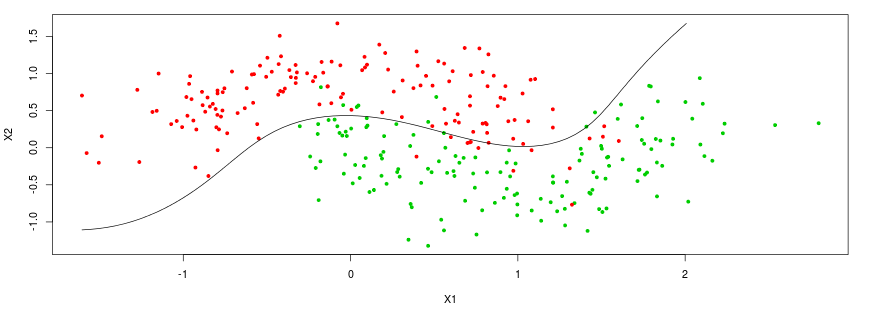
\includegraphics{./Figures/ML/decision_boundary}
     }
	\caption[Two class hypothetical example with non linear decision boundary]{Two class hypothetical example with non linear decision boundary}
	\label{fig:2-class-problem}
\end{figure}

Classification problems may be trivial for humans but are usually quite challenging for automated systems, since we need to deal with a lot of issues such as finding a reasonable number of distinguishing features good enough for classification, that are able to separate the target classes, or finding models that have good generalization capabilities (perform well on unseen data), avoiding overfitting of the model to the training data. Figure \ref{fig:2-class-problem} shows an hypothetical problem with two classes and two features. The main goal is then to find the best decision boundary that results in the best generalization on testing data. 

\begin{figure}[htp]
	\centering
	\resizebox{\textwidth}{!}{
  	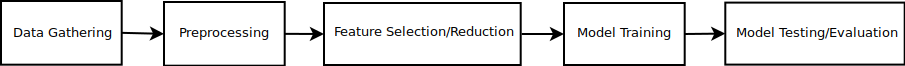
\includegraphics{./Figures/ML/ml-pipeline}
     }
	\caption[Typical pipeline of a machine learning application]{Typical pipeline of a machine learning application}
	\label{fig:ml-pipeline}
\end{figure}
 
Figure \ref{fig:ml-pipeline} shows the workflow of a typical machine learning application. Usually text classification involves steps such as data gathering, preprocessing, feature selection/reduction, training,testing and the final evaluation. The main goal is to assign, with the best accuracy possible, new labels to new documents. 

%Besides, text classification tasks can be divided between single-label or multi-label classification tasks and category-pivoted or document-pivoted text classification. When only one category is to be assigned to documents, it is called single-label classification, otherwise, if multiple labeling is allowed for a single document, it is a multi-label classification. In the case of document-pivoted classification, the goal is to assign one or more categories to a document. On the other hand, in category-pivoted classification the goal is to find all the documents that belong to a category. The former case is more common. This distinction because the set of classes and documents are not always available from the start, i.e, they may be added in different moments in time \citep{Niharika2012TC}. In this work, we are interested in single-classification, document-pivoted tasks.
\subsection{Data Gathering}
The first step is to collect the training and testing data such as sufficient and representative data. This usually implies tasks such as \citep{Gama2015DataMining}:
\begin{itemize}

	\item \textbf{Data Integration} - The initial data might come from different sources, with different formats or duplicated data. This step is important to create a single repository of data. 
    \item \textbf{Data Balancing} - As is often the case with real data, the data is usually not uniformly distributed across the different classes. Consequently, the trained models tend to predict new data with the majority class. Techniques to artificially balance the data might be employed here, such as reducing (Undersampling) / increasing (Oversampling) the number of instances from the majority /minority classes. Another alternative might be performing a stratified sampling in order to keep a significant number of instances in each class. Neighbor-based approaches \citep{mani2003knn,laurikkala2001improving} or synthesization of new examples \citep{chawla2002smote} are popular techniques used in this stage.
    \item \textbf{Cleaning} - The quality of the data is important. Sometimes the data will have missing attributes or useless values. However, redundant or noisy data are important issues to be addressed, such as instances with very similar feature values, attributes easily deducted from others or outliers.
\end{itemize}

Most of these steps were performed by the research team responsible for the data collection. Although, in this work some tasks such as removal of useless data and aggregation of duplicates with different labels were needed.  

\subsection{Preprocessing}
Some learning algorithms do not deal with certain types of data. In order to be able to use them, the type of the attributes might be transformed to another suitable type. For example converting symbolic features to equivalent numeric features, or the other way around. \\ Another important issue to consider is the normalization of the data, such as converting different attributes to the same scale, avoiding the dominance of some attributes and decreasing the dispersion of the data. Some example of used techniques are shown next:

\begin{itemize}
\item \textbf{Standardization} - Standardization transforms each feature by removing their mean and diving non-constant features by their standard deviation, obtaining data normally distributed with zero mean and unit variance ($\rho_{x_{std}}=0$,$\sigma_{x_{std}}=1$)
\[x_{std} = \frac{x - \rho _{X}}{\sigma _{X}}\]
\item \textbf{Normalization} - Normalization involves scaling samples/features vectors to have unit norm, usually achieved by diving by the euclidean norm of the vector.
\[x_{norm} = \frac{x }{\sqrt{\sum_i{x_{i}}^{2}}} \]
\item \textbf{Scaling} - Scaling transform the features to lie between a minimum and a maximum value. Typical ranges are [0,1] or [-1,1]. 
\[x_{[0,1]} = \frac{x - min _{x}}{max _{x} - min _{x}}\]
\end{itemize}

\subsection{Feature Selection}
Feature selection usually involves selecting a subset of the original set of features that provide the biggest discriminatory power, i.e., are able to provide the best separation between classes, result in the best performance of the classifier when trained and avoid the curse of dimensionality. In fact, it has been said in the literature that exists a critical feature dimension from where the performance degrades rapidily \citep{Ribeiro2015CFD}. Feature selection helps in removing irrelevant and redundant features and is usually divided into filter methods, where a subset of features is selected, without considering the predictive model and wrapper methods which use the classifier to rank and choose the best feature set. This step, in conjunction with feature reduction, is likely to be one of the most important steps in the pipeline. The following list shows common techniques employed in feature selection:

%\textbf{Filter Selection Methods}:
\begin{itemize}
	\item \textbf{Information Gain} - Information gain ranks each attribute by its ability to discriminate the pattern classes. Features very informative will provoke the greatest decrease in entropy when the dataset is split by that feature.  
    \[IG(S,A) = H(S) - \sum_{v\in values(A)} \frac{\left | S_v \right |}{\left | S \right |}H(S_v)\]
    The Information Gain $IG$ of a feature $A$ is then equal to the decrease in entropy achieved by splitting the dataset $S$ by feature values $v$ into smaller sets $S_v$, and subtracting from the original entropy $H(S)$ the average entropy of the splits. 
    \item \textbf{Gain Ratio} - The gain ratio is simply the information gain normalized with the entropy of the feature $H(A)$. Since features with many values create lots of branches, creating a bias towards these features, the gain ratio corrects this by taking into account the number and size of branches of a split.
    \[IGR(S,A) = \frac{IG(S,A)}{H(A)}\]
    \item \textbf{Fisher Score} - The Fisher's score select features with high class-separability and low class-variability and is defined by: 
    \[F(x) = \frac{\left | m_1-m_2 \right |^2}{s_1^2+s_2^2}\]
    where $m_1$ and $m_2$ are the means from the feature values (for a 2-class problem) and $s_1$ and $s_2$ are the standard deviations from the feature values of each class.
%     \item \textbf{Minimum Redundancy Maximum Relevance (mRMR)} - The mMRM method\citep{peng2005feature} uses the mutual information as the base to select features which have a high relevance, i.e, a high dependence to the target class and at the same time a minimal redundancy between them.
%     \[max \quad D=\frac{1}{\left | S \right |}\sum_{x_i\in S} I(x_i,c)\]
%     \[min \quad R=\frac{1}{\left | S \right |}\sum_{x_i.x_j\in S} I(x_i,x_j)\]
%     \[max \quad \phi (D,R), \phi = D-R\]
%     The dependency criterion $D$ is computed as the mean of all the mutual information values between the selected features and the target class. On the other hand, the redundancy criterion $R$ is obtained by averaging the mutual information between all the features. The final goal is to maximize the criterion $\phi$, by maximizing $D$ and minimizing $R$.
    \item \textbf{Pearson Correlation} - Pearson correlation can be used to select features that are highly correlated with the target class and features with low correlation between them.  It is a useful measure to see how strongly related two features are. The Pearson correlation gives values between -1 and 1, where absolute values closer to 1 mean a high correlation. The sign indicates whether there is a positive relationship between the variables, that is, if a feature value increase or decreases, the other increases/decreases as well (positive correlation) or if one variable increases/decreases, the other decreases/increases with it (negative correlation). Naturally, we are interested in high absolute values for feature-class relationships and low values feature-feature relationships.  
       
    This Pearson correlation $\rho$ is defined as:
    \[ \rho = \frac{covariance(a , b)}{\sigma _a\times \sigma _b} \]
    where $a$ and $b$ can be both feature vectors or a feature vector and a label vector.
%     \item \textbf{Kruskal-Wallis Test} - This statistical test assess the class-separability of the features and tests whether class groups are drawn from the same population and with the same mean.
%     \[H = \frac{12}{N(N+1)}\sum_{i=1}^{k}\frac{R_{i}^2}{n_i} - 3(N+1)\]
    
    \item \textbf{Chi-Square $\chi^2$ Test} - The Chi-Square test ranks each attribute by computing the $\chi^2$ statistic relative to the target class. This statistic is useful to see if there is an independence relationship between the features and the target class. High values of this statistic means that there is a strong dependence between a particular feature and the target class leading to its selection for classification tasks.
\end{itemize}

% \textbf{Wrapper Methods}:
% \begin{itemize}
% 	\item \textbf{Sequential/Backward Feature Selection} - This method consists of a greedy search that starts with an empty or a full feature set and iteratively adds or removes features that leads to the best or worse classifier performance, when it is added or removed from the feature set, respectively. This process is repeated until a defined number of features is achieved.  
%     \item \textbf{Recursive Feature Elimination} - This method stars with a full set of features and recursively eliminates, in each iteration, the feature with the lowest importance, until a desired set of features is achieved. The method used to compute the feature importances, in each iteration, depends on the classifier. Examples of such methods would be the information gains of a decision tree or the weights assigned to the features by a linear support vector classifier. 
% \end{itemize}
\subsection{Feature Reduction}

Feature reduction is a important step that helps further reducing the dimensionality of the problem, reduces the complexity of the problem and decreases the computational costs. In order to reduce the dimensionality, it is important to keep only the most relevant, informative and discriminative features. Techniques such as Principal Component Analysis (PCA) may be employed in this stage, by aggregating multiple features through linear combinations.

\begin{itemize}
\item \textbf{Principal Component Analysis (PCA)} - PCA is a popular unsupervised (ignores class labels) dimensionality reduction technique that uses linear transformations to find the directions (principal components) with the highest variance. It projects the original data into a lower dimensional space, with the new features retaining most of information. PCA works by finding vectors (called eigenvectors) with the highest amplitude (called eigenvalues) that represent the axes with the highest variance. The original data is then project onto these axes.
% \item \textbf{Linear Discriminant Analysis (LDA)} - LDA is a supervised (uses information from the class labels) algorithm that uses linear transformations to find the directions (linear discriminants) with the highest class-separability while maintaining a low variance within the classes.  Figure \ref{fig:pca_lda} shows examples of poor and good projections that separate poorly and good both classes, respectively. Similar to the PCA method, the original data is then projected onto these directions.  
% \end{itemize}
% \begin{figure}[H]
% 	\centering
% 	\resizebox{\textwidth}{!}{
%   	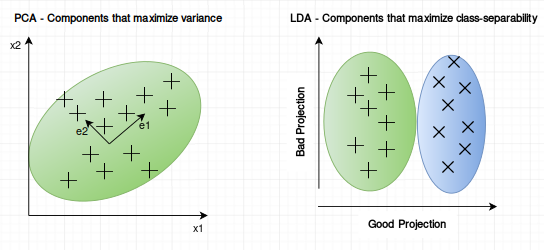
\includegraphics{./Figures/ML/pca_lda}
%      }
% 	\caption[PCA vs LDA]{PCA (left) vs LDA (right)}
% 	\label{fig:pca_lda}
% \end{figure}
\end{itemize}
\subsection{Learning Methods}

After every preprocessing and feature engineering step is completed, comes the learning phase where a set of examples are shown to the classifier, including class labels (supervised learning) or excluding them (unsupervised learning), and the learning process starts. As a result, the classifier is then able to categorize, with a certain accuracy, new unseen data. Some techniques are described bellow:
\begin{itemize}
  \item \textbf{Minimum Distance Classifier} - Minimum Distance Classifiers are template matching system where unseen feature vectors are matched against template prototypes (vectors) representing the classes. This matching usually involves computing the  matching error between both feature vectors using for example the euclidean distance as the error metric. This matching distance can simply be stated as :
  
  \[  \left\Vert  x - m_k \right\Vert \]
 where $x$ is the unseen feature vector and $m_k$ is the feature prototype for class $k$, usually consisting in a feature vector with feature mean values obtained during the training phase. After $k$ tests are performed, the class belonging to the prototype with the minimum distance is chosen. 
  
\item \textbf{k-Nearest Neighbor (kNN)}  - The kNN is a simple and fast unsupervised algorithm that classifies unknown instances based on the majority class from $k$ neighbors. This method starts by constructing a distance matrix between the training samples and the new test sample and chooses the nearest $k$ neighbors. Afterwards, the majority label from these neighbors is assigned to the new data. For two-class problems, $k$ is usually an odd number to prevent ties.

\item \textbf{Naive Bayes} - The Naive Bayes Classifier is a simple supervised probabilistic model based on the Bayes' theorem. The posterior probabilities are computed for each class $wj$ and the class with largest outcome is chosen to classify the feature vector $x$. To achieve this result, the likelihood, prior and evidence probabilities must be calculated, as shown below: 
\[  \text{posterior probability} = \frac{ \text{likelihood}  \cdot \text{prior probability}}{\text{evidence}} \]

\[ P(\omega_j|x) = \frac{p(x|\omega_j) \cdot P(\omega_j)}{p(x)} \]

The main difficulty is to compute the likelihoods $p(x|\omega_j)$ since the other factors are obtained from the data. $P(\omega_j)$ are the prior probabilities and $p(x)$ is a normalization factor which is sometimes omitted. Assuming independence of the features, the likelihoods can obtained as shown bellow:

\[ P(x|\omega_j) = \prod_{k=1}^{d} P(x_k|\omega_j) \]

This simplification allows to compute the class conditional probabilities for each feature separately, reducing complexity and computational costs. 

\item \textbf{Support Vector Machines (SVM)} -  Support vector machines \citep{vapnik1995svm} are optimization methods for binary classification tasks that map the features to a higher dimensional space where an optimal linear hyperplane that separates the existing classes exists. The decision boundary is chosen with the help of some training examples, called the support vectors, that have the widest separation between them and help maximizing the margin between the boundaries of the different classes. The decision surface is in the ``middle'' of these vectors. 
During the training phase, the coefficient vector $w$ and the constant $b$ that define the separating hyperplane are searched such that the following error function is minimized: 

\[ minimize \quad \frac{1}{2} \left \| w \right \|^{2} + C  \sum_{i}^{N} \xi_i \quad s.t  \quad y_i(w \cdot \phi (x_i) + b) \geq 1 - \xi_i  ,\quad \forall x_i \]

where $C$ is an arbitrary constant and $\xi$ are slack variables used to penalize misclassified instances that increase with the distance from the margin. If $C$ is large, the penalty for misclassification is greater. The vectors $x_i$ are the training instances. This method makes use of a kernel function $\phi$ used to transform the input vectors into higher dimensional vectors. New instances are then classified according to which "side" of the hyperplane they are located.

\item \textbf{Decision Tree} - Decision Trees are supervised methods that learn rules based on the training data to classify new instances. The built trees are simple to understand and visualize. During training, each node of the tree is recursively split by the feature that provides, for example, the best information gain.  

\item \textbf{Random Forest} - Random forests ares ensemble methods, i.e., they take into consideration the prediction of several classifiers in order to improve the accuracy and robustness of the prediction results. In the case of random forests, they train a set of random trees with bootstrapped samples (samples drawn with replacement) from the original training data. Each tree is grown by selecting $m$ random features  from the $d$ features and recursively splitting the data by the best splits. The classification of new data is achieved by a majority vote.
\end{itemize}

Each classifier has its own advantages and disadvantages and the right technique should be chosen according to the requirements of the problem-at-hand.
\subsection{Evaluation Metrics}

Experimental evaluation is an important step to assess the effectiveness of a classifier, i.e, the quality of the decisions made by a predictive model on unseen data. In classification tasks, predictions made by a classifier are either considered Positive or False (under some category) and the expected judgments are called True or False (again, under a certain category). Common metrics are \citep{Sebastiani2002MLTC}:

\begin{itemize}
		\item \textbf{Accuracy} - This measure provides a proportion of correctly classified  instances and correctly rejected instances (True Positives and True Negatives) among the whole dataset.
	\begin{figure}[H]
      \centering
    	\[ Acc = \frac{TP + TN}{TP + TN + FP + FN} \]
		\begin{tabular}{lll}
        Acc = Accuracy & TP = True Positives & TN = True Negatives \\ 
        FP = False Positives & FN = False Negatives &
      \end{tabular}
      \end{figure}
      
	\item \textbf{Precision} - This measure provides a proportion of correctly classified  instances (True Positives) among all the positive identified instances (True Positives and False Positives).
	\begin{figure}[H]
      \centering
    	\[ P_i = \frac{TP_i}{TP_i+FP_i} \]
		\begin{tabular}{ll}
        P$_i$ = Precision under Category \textit{i} & TP$_i$ = True Positives under Category \textit{i} \\
        FP$_i$ = False Positives under Category \textit{i} & 
      \end{tabular}
      \end{figure}

    \item \textbf{Recall} - This measure, sometimes called sensitivity, provides a proportion of correctly classified instances (True Positives) among the positive instances that were and should have been correctly identified, i.e., the whole positive part of the dataset (True Positives and False Negatives).\\
      \begin{figure}[H]
      \centering
    	\[ R_i = \frac{TP_i}{TP_i+FN_i} \]
      	\begin{tabular}{ll}
        R$_i$ = Recall under Category \textit{i} & TP$_i$ = True Positives under Category \textit{i} \\
        FN$_i$ = False Negatives under Category \textit{i} & 
      \end{tabular}
      \end{figure}

    \item \textbf{F-measure} - This measure combines precision and recall and provides a balance between them. It is computed as the harmonic mean between the two metrics providing the same weight for both.\\
    \begin{figure}[H]
     \centering
      \[ F_1 = \frac{2 \times P_i \times  R_i}{P_i+R_i} \]
     \begin{tabular}{ll}
        F$_1$ = Harmonic  Mean & P$_i$ = Precision under Category \textit{i} \\
        R$_i$ = Recall under Category \textit{i} & 
     \end{tabular}
     \end{figure}
\end{itemize}

These metrics provides insights on how the model behaves. We can go further and compute the previous estimations in different ways such as:
\begin{itemize}
	\item \textbf{Micro Averaging} - In this case the entire text is treated as a single document and the individual correct classifications are summed up.	\\
    \begin{figure}[H]
      \centering
      \[ P^{\mu} = \frac{\sum_{i=1}^{|C|} TP_i}{\sum_{i=1}^{|C|} TP_i + FP_i} \]
      \begin{tabular}{ll}
        P$^{\mu}$ = Micro Precision, & C = Set of Classes\\
        TP = True Positives, & FP = False Positives
      \end{tabular}
	\end{figure}
    
     \begin{figure}[H]
      \centering
      \[ R^{\mu} = \frac{\sum_{i=1}^{|C|} TP_i}{\sum_{i=1}^{|C|} TP_i + FN_i} \]
      \begin{tabular}{ll}
        R$^{\mu}$ = Micro Recall, & C = Set of Classes\\
        TP = True Positives, & FN = False Negatives
      \end{tabular}
	\end{figure}
    \item \textbf{Macro Averaging} - In this case the precision and recall metrics are computed for each document and then averaged.\\    	
	
	\begin{figure}[H]
      \centering
      \[ P^{M} = \frac{\sum_{i=1}^{|C|} P_i}{|C|} \]
      \begin{tabular}{ll}
        $P^{M}$ = Macro Precision, & C = Set of Classes\\
      \end{tabular}
	\end{figure}
    
    \begin{figure}[H]
      \centering
      \[ R^{M} = \frac{\sum_{i=1}^{|C|} R_i}{|C|} \]
      \begin{tabular}{ll}
        R$^{M}$ = Macro Recall, & C = Set of Classes\\
      \end{tabular}
	\end{figure}
\end{itemize}

In addition to the previous averages, the standard deviation is a common dispersion metric that may be computed as follows:
    \begin{figure}[H]
      \centering
\begin{tabular}{ll}
		\Large
		\( \sigma = \frac{1}{N-1}\sum_{i=1}^{|N|}{(x_i - \bar{x})^2} \) & \\
		\\
        N = Number of samples, & x$_i$ = Result of the i-th measurement \\
		$\bar{x}$ = Arithmetic mean of the N results
      \end{tabular}
\end{figure}

These evaluation methods can give different results. Macro averaging gives equal weights for each class, even if there are unbalanced classes. On the other hand, micro averaging gives equal weight to the documents under evaluation, but it can happen that large classes dominate smaller classes. Therefore, macro averaging provides a sense of effectiveness on small classes, increasing their importance. Usually, the choice of which method to use depends on the requirements of the application.

\begin{itemize}
\item \textbf{Receiver Operating Characteristics (ROC)} - ROC curves \citep{Fawcett2006ROC} are useful graphs to visualize the performance of binary classifiers. They are useful to compare the rates at which the classifier is making correct predictions (True Positive Rate plotted on the Y axis) against the rate of false alarms (False Positive Rate plotted on the X axis). Important points in this graph are the lower left point (0,0), representing a classifier that never classify positive instances, neither having False Positives or True Positives. On the other hand, the upper right point (1,1) represents a classifier that classifies every instance as positive, disregarding if it is a false positive or not. Finally, the point (0,1) represents the perfect classifier, where every instance was correctly classified. Figure \ref{fig:roc} illustrates this idea, showing three hypothetical classifiers and the regions of good and poor performance, which are above or below the line defined by a random classifier making correct random guesses half of the time.  The area bellow the ROC curve is called Area Under the Curve (AUC) and is also a good measure. A perfect classifier would have an AUC of 1.0 while a random classifier would only have 0.5.

\begin{figure}[htp]
	\centering
	\resizebox{\textwidth}{!}{
  	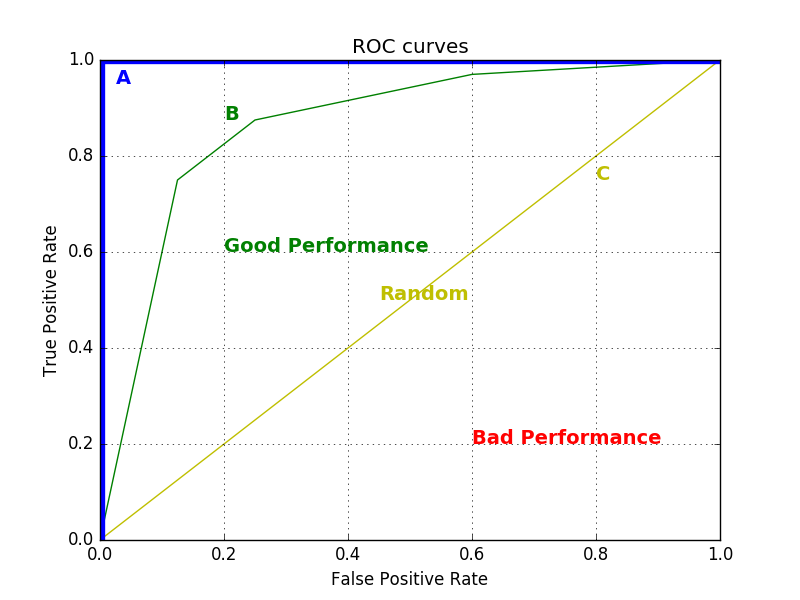
\includegraphics{./Figures/ML/roc}
     }
	\caption[ROC curves of 3 hypothetical classifiers]{ROC curves of 3 hypothetical classifiers: Perfect (A), good (B) and random (C)}
	\label{fig:roc}
\end{figure}

\item \textbf{Precision-Recall Curves (PR)} - The Precision-Recall Curve plots the trade-off between the precision and recall achieved by a classifier, by showing the recall on the X axis and precision on the Y axis. An important point in this graph is the upper right point (1,1) which represents the ideal classifier having maximum precision and recall. Figure \ref{fig:pr} shows three hypothetical classifiers and the areas of good and bad performance, which are above or below the line defined by a random classifier. The area bellow the PR curve is called Average Precision (AP) and is also a good measure. A perfect classifier would have an Average Precision of 1.0 while a random classifier would only have 0.5. 

\begin{figure}[htp]
	\centering
	\resizebox{\textwidth}{!}{
  	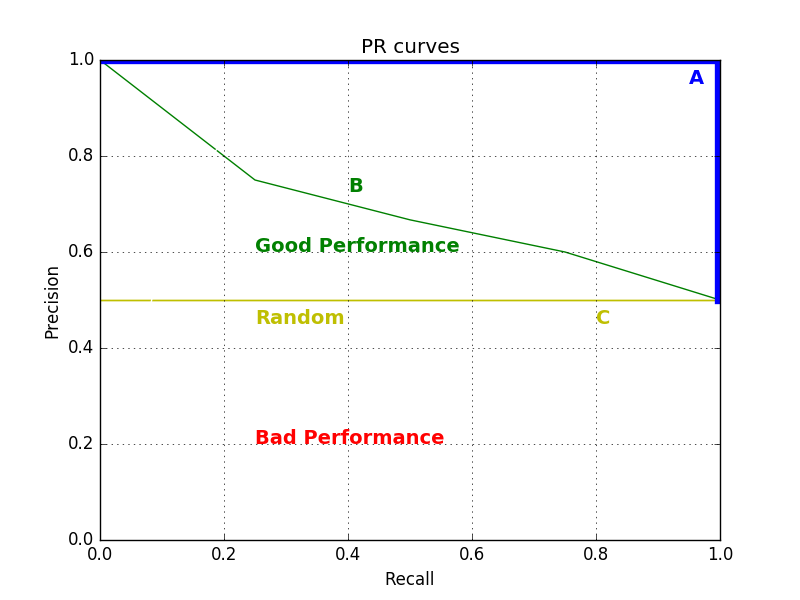
\includegraphics{./Figures/ML/pr}
     }
	\caption[Precision-Recall curves of 3 hypothetical classifiers]{Precision-Recall curves of 3 hypothetical classifiers: Perfect (A), good (B) and random (C)}
	\label{fig:pr}
\end{figure}

\item \textbf{Stratified K-fold Cross Validation} - A popular technique to evaluate the performance of the system is to split the data into training and testing sets, using the later to estimate the true generalization performance of the classifier. However, this may bring some issues such as the trade-offs between the percentage splits or the representativity of the test set \citep{Polikar2006PR}. A popular accepted approach is to split the entire dataset into $k$ representative partitions, using $k-1$ of these partitions for training and the remaining one for testing. This process is then repeated $k$ times, (each time using a different test partition) and the results averaged. 
\end{itemize}

% https://gate.ac.uk/sale/tao/splitch10.html#x14-26300010
% https://gate.ac.uk/sale/tao/splitch19.html#x24-45300019.1
% http://www.cse.unsw.edu.au/~billw/mldict.html
% http://nlp.stanford.edu/IR-book/html/htmledition/text-classification-and-naive-bayes-1.html
% http://arxiv.org/pdf/cs/0110053.pdf
% http://www.aaai.org/ojs/index.php/aimagazine/article/view/406/342


\section{Relation to this work}

In this chapter we started by defining some classical notions about relevance and how it is a concept well studied in academic disciplines such as Information Retrieval. However, it should be noted that these classical views are not aligned with the approach of this work. Instead, we explore another direction by defining relevance in terms of journalistic criteria, such as: controversialness, interestingness, meaningfulness, novelty, reliability and scope. According to the relation between the previous attributes, a document should be classified as relevant or irrelevant. Likewise, we can treat these attributes as their own sub-problems. \\
The presented NLP tasks are also a crucial part of this work, since they provide the features to be used in the classification experiments. Since the type of our study object is raw text, the NLP field comes as a natural choice in tackling the problem of feature extraction. \\
We also reviewed some important pattern recognition concepts. First, we define our task as a binary problem, which has to classify text documents as either relevant or irrelevant. It is important to note that mentioned sub-problems are also binary problems by themselves, meaning that a document can be classified as controversial or not uncontroversial, interesting or uninteresting, meaningful or meaningless, new or old, reliable or unreliable and finally wide or narrow. Since we are dealing with text, a common problem is the high dimensionality of the feature space. Therefore, we may use well known techniques to reduce the problem to its most important, informative and discriminatory attributes. Finally, we use learning and evaluation methods to build and evaluate the accuracy our models.

Table \ref{tab:methods-used} summarizes this view by presenting the used journalistic relevance criteria, the used natural language processing tasks and machine learning methods used. 


\begin{table}[H]
\centering
\resizebox{\textwidth}{!}{%
\begin{tabular}{c|c|ccccc}
\hline
\multicolumn{1}{|c|}{\textbf{Definition  of Relevance}} & \textbf{NLP Tasks} & \multicolumn{5}{c|}{\textbf{Machine Learning Methods}} \\ \hline
\multicolumn{1}{|c|}{\textbf{Criteria}} & \textbf{Extraction} & \multicolumn{1}{c|}{\textbf{Preprocessing}} & \multicolumn{1}{c|}{\textbf{Selection}} & \multicolumn{1}{c|}{\textbf{Reduction}} & \multicolumn{1}{c|}{\textbf{Models}} & \multicolumn{1}{c|}{\textbf{Evaluation}} \\ \hline
\multicolumn{1}{|c|}{Controversialness} & Part-of-Speech & \multicolumn{1}{c|}{Standardization} & \multicolumn{1}{c|}{Info. Gain} & \multicolumn{1}{c|}{PCA} & \multicolumn{1}{c|}{MDC} & \multicolumn{1}{c|}{Accuracy} \\ \hline
\multicolumn{1}{|c|}{Informativeness} & Chunking & \multicolumn{1}{c|}{Normalization} & \multicolumn{1}{c|}{Gain Ratio} & \multicolumn{1}{c|}{} & \multicolumn{1}{c|}{kNN} & \multicolumn{1}{c|}{Precision} \\ \cline{1-4} \cline{6-7} 
\multicolumn{1}{|c|}{Meaningfulness} & Named Entities & \multicolumn{1}{c|}{Scaling} & \multicolumn{1}{c|}{Fisher} & \multicolumn{1}{c|}{} & \multicolumn{1}{c|}{NB} & \multicolumn{1}{c|}{Recall} \\ \cline{1-4} \cline{6-7} 
\multicolumn{1}{|c|}{Novelty} & Polarity of words & \multicolumn{1}{c|}{} & \multicolumn{1}{c|}{Pearson} & \multicolumn{1}{c|}{} & \multicolumn{1}{c|}{SVM} & \multicolumn{1}{c|}{F$_1$} \\ \cline{1-2} \cline{4-4} \cline{6-7} 
\multicolumn{1}{|c|}{Reliability} & LDA topics & \multicolumn{1}{c|}{} & \multicolumn{1}{c|}{Chi-square} & \multicolumn{1}{c|}{} & \multicolumn{1}{c|}{DT} & \multicolumn{1}{c|}{ROC} \\ \cline{1-2} \cline{4-4} \cline{6-7} 
\multicolumn{1}{|c|}{Scope} & N-gram &  &  & \multicolumn{1}{c|}{} & \multicolumn{1}{c|}{RF} & \multicolumn{1}{c|}{AP} \\ \cline{1-2} \cline{6-7} 
 & Stemming &  &  &  & \multicolumn{1}{c|}{} & \multicolumn{1}{c|}{k-Fold-CV} \\ \cline{2-2} \cline{7-7} 
 & Lemmatization &  &  &  &  &  \\ \cline{2-2}
\end{tabular}%
}
\caption[Methods used in this work]{Methods used in this work}
\label{tab:methods-used}
\end{table}




%----------------------------------------------------------------------------------------

%----------------------------------------------------------------------------------------





 
% Chapter 3
\chapter{State of the Art} % Main chapter title
%\epigraph{A fancy quote}{Me}

\label{art} % For referencing the chapter elsewhere, use \ref{Chapter2} 
\lhead{Chapter 3. \emph{State of the Art}} % This is for the header on each page - perhaps a shortened title

In this chapter we perform a review of the literature, i.e., a review of the techniques most used to solve text classification problems. This chapter is divided into two main sections. In the first section we explore techniques used in the scientific literature. We then proceed to the second section where we give a technological review. This last section shows the difference between studying practical applications that solve real-world problems and theoretical models of the reality.

%----------------------------------------------------------------------------------------

\section{Scientific Overview}

Over the past decades, a large number of techniques has been applied to the automatic classification of text with varied success. Although there is no accepted solution yet that can globally solve the problem, there are many interesting approaches to tackle the problem. In this section we make a short survey of different approaches. We also present some standard data sets useful to determine which techniques are in general the best computational methods. 


\subsection{Approaches to Social Media Text Classification}

Huge quantities of information are spread everyday through social networks.
Acknowledging the fact that users, alone, are unable to deal with so much information, automatic methods have been developed to classify social media posts according to different aspects~(e.g. sentiment~\citep{Preslav2013SemEval}, categories~\citep{Bharath2010TwitterFiltering}, mentioned events~\citep{Ritter2012OpenDomain},popularity~\citep{Bharath2010TwitterFiltering,Fernandes2015PredictingPopularity} or virality~\citep{guerinietal2011TextVirality} of the content).
The previous methods can be used by content-based recommender systems \citep{lops2011recommendersystems}, and would hopefully help users to organize their content and filter unwanted information.

Our work falls in the previous category of automatic approaches for the classification of social media text, in this case, focusing on its relevance to a wide audience, from a journalistic point of view. Previous work has explored the virality of social network posts~\citep{guerinietal2011TextVirality} and attempted to define certain phenomena in their messages, namely: virality~(number of people that access it in a given time interval), appreciation~(how much people like it), spreading~(how much people share it), white and black buzz~(how much people tend to comment it in a positive or negative mood), raising discussion~(the ability to induce discussion among users) and controversy~(the ability to split the audience into those that are pro and those against).
Some of the previous phenomena might also have impact on the relevance of a post.

After defining those phenomena\citep{guerinietal2011TextVirality}, the same authors developed a SVM-based classifier for automatically predicting them in posts of the social platform Digg, based only on the lemmas of the content words in the story and snippet.
They reached $F_1$ measures of 0.78 for appreciation, 0.81 for buzz, 0.70 for controversiality, and 0.68 for raising-discussing.

Others have also relied on a SVM to classify consumer reviews as helpful or not~\citep{Ching2013SocialNLP}.
For that purpose, 1 to 3-grams were exploited, together with the length of the review, its degree of detail, the given rating, and specific comparison-related keywords. With the best configuration, their accuracy reached 0.72.

The phenomena of popularity has some connections both with virality and relevance.
In fact, the prediction of popularity of web content has been surveyed elsewhere~\citep{Tatar2014PredictPopularity}.
Most research on the topic has focused on the interactions of users~(e.g. reads, appreciation, comments, shares)~\citep{Szabo2010PredictPopularity}. Yu et al. \citep{Yu2011PopularityMarketingMessages} used SVMs and Naive Bayes classifiers to predict the popularity of social marketing messages, achieving accuracies of 0.72 and 0.68, respectively. The used data was gathered from Facebook posts produced by top restaurant chains and labeled as ``popular'' or ``not popular'' according to the number of likes.  The feature sets used consisted simply of word vectors using bag-of-words representations. In fact, they found that words such as ``win'', ``winner'', ``free'' or ``fun'' were rated as less popular. However, words such as ``try'', ``coffee'', ``flavors'' or ``new'' were  rated as more popular. To rank these words, they used a SVM classifier which used only boolean features representing the presences or absences of the words. Such words were found to be the most discriminant when classifying content as popular or not popular.   

Based on the category of a news article, subjectivity of language used, mentioned named entities and the source of the publisher, Bandari et al.~\citep{Bandari2012ForecastingPopularity} achieved an overall accuracy of 0.84 on predicting the number of tweets that would mention it. An acceptable popularity measure is the number of times a publication is mentioned in other publications. Especially based on the features of an author of a tweet~(e.g. followers, favorites), Petrovic et al.~\citep{Petrovic2011MsgProgagation} predicted whether it would be retweeted or not, with an F$_1$ measure of about 0.47. Hong et al. \citep{Hong2011PredictingTwitter} also addressed the same problem achieving an F$_1$ score of 0.60. They used content features such as TF-IDF scores and LDA topic distributions; topological features such as PageRank scores and reciprocal links; temporal features such as time differences between consecutive tweets, average time difference of consecutive messages and average time for a message to be retweeted and finally meta information features such as whether a message has been retweeted before or the total number of tweets produced by an user. 

Fernandes et al.~\citep{Fernandes2015PredictingPopularity} exploited a large set of features to predict the popularity of Mashable news articles, based on the number of times they would be shared.
Considered features included the length of the article, its title and its words, links, digital media content, time of publication, earlier popularity of referenced news, keywords of known popular articles, and several NLP features, such as topic, subjectivity and polarity.
The best F$_1$ measure~(0.69) and accuracy~(0.67) was achieved with a Random Forest classifier.

Only based on the tweets content, tweets mentioning trending topics were classified as related or unrelated (e.g.~spam) with a F$_1$ score of 0.79, using a C4.5 classifier, and 0.77, using a Naive Bayes, which also takes less time to train~\citep{Irani2010TrendStuff}. Lee et al. \cite{Lee2011TrendingTopic} also address the problem of assigning trending topic to categories. By using TF-IDF word vector counts, they achieved accuracies of 0.65 and 0.61 by using Naive Bayes and SVM classifiers, respectively.     
In order to detect the context from which certain tweets belong, Genc et al. \citep{Genc2011ClassifyingTweets} gathered a set of tweets belonging to three different categorical events and tried to classify them by finding clusters of similar tweets, achieving an average accuracy of 0.86. In order to compute the similarity between tweets they used different methods such as string edit distances and distances between associated Wikipedia articles (for each tweet), as indicators of the distance between two tweets. This distance was computed as the shortest path lenght, between the two wikipedia articles, in the categorical data graph from Wikipedia.

The limitations of traditional bag-of-word classification models in microblogging platforms have been pointed out, due to the short length of documents~\cite{Bharath2010TwitterFiltering}.
Alternatively, other features can be used, including the author's name, presence of shortening of words and slangs, time-event phrases, opinioned words, emphasis on words, currency and percentage signs and user mentions at the beginning and within the post.
The previous features were used to classify tweets into a set of categories (News, Events, Opinions, Deals, and Private Messages) with an accuracy of 0.95. When combined with a bag-of-words, there are no improvements. In fact, the author's name seemed to be the most relevant feature. 

Figueira et al. \citep{Figueira2016RelevanceDetection} used a reduced set of features in order to classify social media posts from Google+, Youtube and Twitter, according to their relevance. The feature set included normalized length of posts, number of occurrences of typical certain words, such as swear words, the use of excessive punctuation and smileys/emoticons. They also used two customized bag-of-words that are more likely to appear in news and do not appear in chat and vice-versa, achieving a final F$_1$ score of 0.68.

Frain and Wubben \citep{Frain2016SatiricLR} developed a satirical dataset which contained articles labeled as Satire or Non Satire. Using features like profanity amounts, punctuation amounts, positive and negative word counts, bag-of-words models using unigrams and bigrams they achieved a F$_1$ score of 0.89 using support vector classifiers.	

Liparas et al.\citep{Liparas2014NewsClassification} address the problem of classifying web pages by topic (Business, Lifestyle, Science or Sports), by extracting textual and visual features. Textual features included N-grams, ranging from unigrams to four-grams. Using random forests, they obtained an average F$_1$ score of 0.85 and an accuracy of 0.86. Kinsella et al. \citep{Kinsella2011TopicClassification} also investigate this problem by using additional metadata retrieved from hyperlinks. They used text from message boards as the object of analysis. By using a simple bag-of-words representation as the feature vectors, they classified each concatenation of a post plus the metadata retrieved from external links with a Multnominal Naive Bayes obtaining an F$_1$ score of 0.90, showing a clear improvement when using only the content of the message (0.85).  

Although with a different goal, the previous works have focused on classifying social media posts automatically, according to some criteria, some of which~(virality, helpfulness, popularity, etc) related to our target goal, relevance, due to their context-dependence and ambiguous nature.
Our approach is also similar, as we rely on the extraction of a set of features from each post and then apply a set of algorithms to learn a classifier based on those features. In our case, only text and linguistic-related features are used.

\section{Technological Overview}
In the following sections we present a small survey of practical tools currently available and available datasets. There is a wide range of frameworks and libraries available that can be used to process languages and extract information. Usually they can be divided in general purpose tools or systems developed in research contexts where a specific problem is addressed. 

\subsection{Common Data Sets}

Many different methods were developed to solve linguistic tasks. In order to evaluate the performance of the developed systems and to determine the best approaches, it is important to have the same terms of comparison like annotated data ready to test and use. This way, the comparison of results is more reliable since the systems are tested in the same settings. Therefore, the need for standard formats that allow to replicate experiments, easy exchange of data and testing of algorithms on standard corpora is an important issue.\\
Many corpora have been developed in order to express in a clear and precise way real-life data. Currently there are some datasets commonly used by the NLP community, like large collections of annotated text and tree banks. We summarize the most popular available collections usually used for text categorization and machine learning applications:

\begin{itemize}
	%\item \textbf{\href{https://catalog.ldc.upenn.edu/byyear.jsp}{LDC}} - Each year, the Linguistic Data Consortium provides a variety of different corpora in different languages, ranging from data made available in Conferences on Natural Language Learning (CoNLL), treebanks,  broadcast news, among others.
    %\item \textbf{\href{http://catalog.elra.info}{ELRA}} -  ELRA provide many language resources like corpora, lexicons and terminology written in a wide range of languages.
    %\item \textbf{\href{http://catalog.elra.info}{ICAME}} - ICAME is an archive of many English text corpora such as the Brown Corpus and the Lancaster Corpus.
    \item \textbf{\href{http://trec.nist.gov/data/reuters/reuters.html}{Reuters Corpora}} - The Reuters corpora, distributed by NIST, is a large collection of news stories used in development and testing of NLP and ML systems.
    \item \textbf{\href{http://ota.ox.ac.uk/catalogue/index.html}{OTA}} - OTA is a collection of literary English texts that can be used as linguistic corporas.
    \item \textbf{\href{http://www.elsnet.org/resources/eciCorpus.html}{ECI/MCI}} - The European Corpus Initiative offers a great collection of texts written in many different languages. They offer these resources for research purposes at low cost.
    \item \textbf{\href{http://www.elsnet.org/resources/eciCorpus.html}{ICE}} - ICE  is a large collection of English texts with many regional varieties. Each corpus follows a well-defined corpus design as well common grammatical and textual annotations.
    \item \textbf{\href{http://qwone.com/~jason/20Newsgroups}{20 Newsgroups Data Set}} - The 20 newsgroups data set is a well-known collection. It consists of a large number of documents partitioned across different categories.
    \item \textbf{\href{http://www.cs.cmu.edu/~webkb}{WebKB Collection}} - The WebKB project aims to translate the the web content to a symbolic representation better understandable by computers. They provide large collections of web pages classified under a set of categories. 
    \item \textbf{\href{http://quod.lib.umich.edu/m/micase/}{MICASE}} - The MICASE collection contains many texts of spoken English, categorized under the speaker attributes (Position, Status, First language) and the transcript attributes (Interactivity, Discipline, Event).
    \item \textbf{\href{http://www.ling.upenn.edu/hist-corpora/PPCME2-RELEASE-3/index.html}{PPCME}} - The PPCME offers large collections of simple text, PoS tagged text and syntactically annotated text. The text comes from samples from the British English prose across the history and its annotations are reviewed by expert human annotators.
    \item \textbf{\href{http://www.cs.cmu.edu/~webkb}{CoNLL Data Sets}} - The ConNLL yearly conference usually provides annotated train and test data sets for its shared tasks. These shared tasks usually include annotated data related to the chosen topic such as grammatical correction, coreference, syntactic and semantic dependencies, name entity recognition, chunking, among others.
    \item \textbf{\href{http://trec.nist.gov/data/tweets}{Tweets2011 Corpus}} - Tweets2011 was a microblog track from TREC conference and they used data provided by Twitter for testing. This data contains millions of tweets sampled across two weeks, containing both important and spam messages.
    \item \textbf{\href{http://clic.cimec.unitn.it/amac/twitter_ngram}{RTC Corpora}} - The Rovereto Twitter Corpus is a collection of millions of annotated tweets. Each tweets is classified by the genre of the author.
    \item \textbf{\href{http://mpqa.cs.pitt.edu/corpora}{MPQA Corpora}} -The MPQA is a set of manually annotated collections such as opinion corpus, debate corpus, arguing corpus and good/bad corpus.
    \item \textbf{\href{http://nlp.uned.es/replab2013}{RepLab}} - In recent years, RepLab proposed an evaluation framework for providing and evaluating automatic tools for the problem of Online Reputation management. The RepLab 2013 dataset consists of manually annotated tweets, gathered from the 1st June 2012 till the 31st Dec 2012, related to a selected set of entities. This data is part of a competitive monitoring task, consisting of four main evaluation tasks, such as: Filtering tweets according to their relation to a specific entity (related/unrelated), polarity of the tweet (positive, negative or neutral) in relation to a particular entity, topic detection and topic priority \citep{replab2013overview}. 
\end{itemize}

\subsection{Related Comparisons}

Gonz{\'a}lez \citep{gonzalez2015Colloquialanalysis} highlights the particular characteristics of Twitter messages that make common NLP tasks challenging, such as irregular grammatical structure, language variants and styles, out-of-vocabulary words or onomatopeias, reminding the fact that there is still a lack of gold standards regarding colloquial texts, especially for less-resourced languages. Therefore, preprocessing techniques are usually employed as an initial step. Clark \citep{Clark2003preprocessing} developed a tool that applies a set of tasks to noisy text coming from Usenet news. This tool follows an integrated approach where it identifies boundaries between tokens and sentences, corrects spelling mistakes and identifies wrong capitalizations. Wong et al. \citep{Wong2008Dirtytexts} developed a spelling correction preprocessing system as part of a system that builds an ontololgy from text coming from chat records. Besides, this system also expands abbreviations and corrects improper casing. In order to achieve this, the system tokenizes the input text and computes a sorted list of corrected suggestions for each erroneous word identified by the system.

Besides comparing different NLP tools, we also analyze their performance in different types of text, some more formal, from newspapers, and some less formal, from Twitter. Similar comparisons, though with different goals, were performed by others. For instance, in order to combine different NER tools and improve recall, Dlugolinsk{\'y} et al. \citep{Dlugolinsk2013CombiningNER} assessed selected tools for this task in the dataset of the MSM2013 task.
This included the comparison of well-known tools such as ANNIE\footnote{\url{https://gate.ac.uk/sale/tao/splitch6.html\#chap:annie}}, OpenNLP\footnote{\url{https://opennlp.apache.org}}, Illinois Named Entity Tagger\footnote{\url{https://cogcomp.cs.illinois.edu/page/software_view/NETagger}} and Wikifier\footnote{\url{https://cogcomp.cs.illinois.edu/page/software_view/Wikifier}}, OpenCalais\footnote{\url{http://www.opencalais.com}}, Stanford Named Entity Tagger\footnote{\url{http://nlp.stanford.edu/software/CRF-NER.shtml}} and Wikipedia Miner\footnote{\url{http://wikipedia-miner.cms.waikato.ac.nz}}.

Additional work by Dlugolinsk{\'y} et al. \citep{dlugolinsky2013evaluation} used the same evaluation dataset, adding LingPipe\footnote{\url{http://alias-i.com/lingpipe}} to the set of assessed tools. The authors used GATE\footnote{\url{https://gate.ac.uk}} as the evaluation framework considering strict and lenient matchings, depending on whether responses were fully or partially correct, respectively. OpenCalais achieved the best $F_1$ scores for the LOC (0.74), MISC (0.27) and ORG(0.56) entities while Illinois NER performed better on the PER (0.79) entity. However, LingPipe got the weakest $F_1$ scores in the LOC (0.30), ORG (0.07) and PER (0.35) entities. Stanford NER was the weakest in identifying MISC (0.05) entities.

Godin et al. \citep{godin2013leveraging} also used the MSM2013 challenge corpus and performed similar evaluations oriented to NER web services, such as AlchemyAPI\footnote{\url{http://www.alchemyapi.com}}, DBpedia Spotlight\footnote{\url{https://github.com/dbpedia-spotlight/dbpedia-spotlight}}, OpenCalais, and Zemanta\footnote{\url{http://www.zemanta.com}}. Since the evaluated services use complex ontologies, a mapping between the obtained ontologies and entity types was performed, with good $F_1$ scores when using AlchemyAPI for the person (0.78) and location (0.74) type entities, and OpenCalais for the organization (0.55) and miscellaneous (0.31) entities.
Rizzo et al. \citep{rizzo2012nerd} also evaluated web services, such as Lupedia\footnote{\url{http://dbpedia.org/projects/lupedia-enrichment-service}}, Saplo\footnote{\url{http://saplo.com}}, Wikimeta\footnote{\url{https://www.w3.org/2001/sw/wiki/Wikimeta}} and Yahoo Content Analysis (YCA), but with focus on different kinds of well-formed content and varying length, such as TED talks transcripts, New York Times articles and abstracts from research papers. In fact, they evaluated the resulting NER and Disambiguation (NERD) framework, which unified the output results of the aforementioned web services, supporting the fact that tools such as AlchemyAPI, OpenCalais and additionally DBpedia Spotlight perform well in well-formed contents, using formal language. Rizzo et al. also report on the evaluation of datasets with colloquial text, namely Twitter text from the MSM2013 challenge and newspaper text from the CoNLL-2003 Corpus \citep{rizzo2014benchmarking}. They report better NER results when using a combination of the tested tools, achieving $F_1$ results greater than 0.80 on he CoNLL-2003 dataset, for all entity types and $F_1$ results greater than 0.50 on the MSM-2013 dataset, except for the miscellaneous type that obtained results less than 0.30.

Garcia and Gamallo \citep{Garcia2015Slate} report the development of a multilingual NLP pipeline. To assess the performance of the presented tool, they performed experiments with POS-tagging and NER. The POS-tagger performed slightly better than well-known tools such as OpenNLP and Stanford NER, achieving a precision score of 0.94 on the Brown Corpus. On the other hand, the NER module achieved $F_1$ scores of 0.76 and 0.59 on the IEER\footnote{\url{http://www.itl.nist.gov/iad/894.01/tests/ie-er/er_99/er_99.htm}} and SemCor\footnote{\url{http://www.gabormelli.com/RKB/SemCor_Corpus}} Corpus, respectively.\\
Rodriquez et al. \citep{rodriquez2012comparison} and Atdag and Labatut \citep{atdag2013comparison} compared different NER tools applied to different kinds of text, respectively biographical and OCR texts. Rodriguez et al. used Stanford CoreNLP, Illinois NER, LingPipe and OpenCalais, on a set of Wikipedia biographic articles annotated with person, location, organization and date type entities. Due to the absence of biography datasets, the evaluated corpus was fully designed by the authors, i.e., the evaluated corpus consisted of a series of Wikipedia articles which were annotated with the aforementioned entity types.  Although CoreNLP obtained the best $F_1$ scores~(0.60 and 0.44) in two manually-annotated resources, there was not a tool that outperformed all the others in every entity type. They are rather complementary. Atdag and Labatut evaluated OpenNLP, Stanford CoreNLP, AlchemyAPI and OpenCalais using datasets with the entity types person, location and organization manually annotated. They used data from the Wiener Library, London and King’s College London’s Serving Soldier archive, which consisted of Holocaust survivor testimonies and newsletters written for the crew of H.M.S. Kelly in 1939. Once again, Stanford CoreNLP gave the best overall $F_1$ results (0.90) while OpenCalais only achieved 0.73.

\subsection{A Review of Current Tools}
\label{nlp_tools}

In order to choose the correct tools for the job, many criteria have to be considered. Usually good systems should be be open source, well-documented, extensible and easy to adapt. Each tool has different features, work under different programming languages and setups or have different learning curves. In the following list we detail common frameworks and libraries used to develop NLP systems and, in some cases integrating them to a machine learning pipeline. They are described and grouped in ``standard'' toolkits, which means they were developed with no specific kind of text in mind, and social network-oriented tools, which aim to be used in short messages from social networks.

\textbf{Standard NLP toolkits:}
\begin{itemize}
    \item \textbf{\href{http://www.nltk.org/}{NLTK}} - The NLTK toolkit is a Python library developed within a coursed taught at the University of Pennsylvania with good design goals in mind such as simplicity, modularity and extensibility. The library is divided in independent modules responsible for specific NLP tasks such as tokenization, stemming, tree representations, tagging, parsing and visualization. It also comes bundled with popular corpus samples ready to be read. By default, NLTK uses the Penn Treebank Tokenizer, which uses regular expressions to tokenize the text. Its PoS tagger uses the Penn Treebank tagset and is trained on the Penn Treebank corpus. %with a Maximum Entropy model.
The Chunker and the NER modules are trained on the ACE corpus. %with a Maximum Entropy model. 
It also includes modules for text classification, providing methods for feature encoding, selection and standard classifiers \citep{Loper2002NLTK,Bird2006NLTK}.

    \item \textbf{\href{https://opennlp.apache.org}{Apache OpenNLP}} - OpenNLP is a Java library that uses machine learning methods for common natural language tasks, such as tokenization, POS tagging, NER, chunking and parsing. It can be used out-of-the-box since it comes bundled with pre-trained models for different tasks ready for use. Besides, it is extensible, has built-in support of many corpora formats and it is accessible by both application and command line interfaces. Users can also train their own models.% with Perceptron or Maximum Entropy methods, and use them instead. 
The pre-trained models for English PoS tagging and chunking use the Penn Treebank tagset. The Chunker is trained on the CoNLL-2000 dataset. The pre-trained NER models cover the recognition of persons, locations, organizations, time, date and percentage expressions. A classifier and evaluation metrics are also included.

    \item \textbf{\href{http://stanfordnlp.github.io/CoreNLP}{Stanford CoreNLP}} - The CoreNLP toolkit is a straightforward JAVA pipeline that provides common natural language processing tasks.  CoreNLP was build with simplicity and reliability in mind, i.e., simple to set up run, since users do not need to learn and understand complex installations and procedures seen in other bigger and complex systems, like GATE \citep{Cunningham2002GATE} or UIMA \citep{Ferrucci2004UIMA}. The most supported language is English, but other languages are also available \cite{Manning2014CoreNLP}. Basically, the tool is fed with raw text and afterwards a series of annotator objects add information resulting in a complete language analysis. This pipeline can then easily be integrated in larger systems, as a component, that the user may be developing. The CoreNLP tool performs a Penn Treebank style tokenization and the POS module %is an implementation of the Maximum Entropy model 
uses the Penn Treebank tagset. The NER %component uses a Conditional Random Field (CRF) model and 
component uses a model trained on the CoNLL-2003 dataset. 
    
    \item \textbf{\href{https://spacy.io}{SpaCy}} - SpaCy is a library used for NLP written in Python/Cython. The main goal is to be a reliable alternative to common toolkits like NLTK and others that usually are more suitable for educational or research purposes. This way, it can be used within industrial environments, like small companies, that usually requires great speed, accuracy, documentation and concise APIs. The fact that is written in Cython (language that compiles to C or C++) makes it faster than other well-known tools. According to recent research SpaCy has one of the fastest systems\citep{honnibal2015spacy,Choi2015DependencyParserComparison}.% However, there seems to be a trade-off with the accuracy of the results \citep{Choi2015DependencyParserComparison}.
    
    \item \textbf{\href{http://www.clips.ua.ac.be/pages/pattern}{Pattern}} - The Pattern tool is a Python library that provides modules for web mining, NLP and ML tasks. A common workflow is to use the methods to extract data from the web (using the provided methods to access well-known APIs from common services) and perform some processing on the data afterwards to get results. The goal of the library is not providing methods for a single field but rather a general cross-domain and ease-of-use functionality \citep{Smedt2012Pattern}.
    
    \item \textbf{\href{https://gate.ac.uk}{GATE}} - GATE is a well-known architecture and flexible framework used to design and develop natural language applications. It provides baseline methods for language processing, including measurement of its performance and works under open standards like JAVA and XML. The GATE frameworks stands on three types of independent components: Language Resources (corpora, 1exicons), Processing Resources (NLP algorithmic tasks, evaluation, pluggable ML implementations) and Visual Resources. A great characteristic of the GATE framework is that the core system is broken into smaller components that can be used, extended or replaced. The user has a a wide range of possible configurations to work with. Besides, the user can choose to use standard package ANNIE, which already encompasses many common NLP tasks, or choose to create its own set of coupled components to make a new application \citep{Cunningham2002GATE}.
    \item \textbf{\href{http://uima.apache.org}{UIMA}} - The UIMA framework is a distributed middleware architecture similar to the GATE framework, used to develop NLP analysis engines that deal with large volumes of unstructured data. Originally developed by IBM Research and now maintained by the Apache Software Foundation, UIMA has four main modules: Acquisition, Unstructured Information Analysis (UIA), Structured Information Access (SIA) and Component Discovery (CD). \\ The acquisition module is responsible for gathering data from external sources where web crawlers may employ this functionality. The UIA module is responsible for processing the data through Text Analysis Engines (TAE), similar to the Processing resources in GATE. This module is divided in smaller components, each responsible for a NLP task. Each document is then attached to an analysis report forming a structure called Common Analysis Structure (CAS). The results of the UIA modules provide structured information (indexes, dictionaries, ontologies, etc) for the SIA module, which can then be reused by the UIA module, creating a feedback loop between these two components. This module is further divided into semantic search, structured knowledge access and document metadata access components. Finally, the CD module provides mechanism to find the right component required for a specific task \citep{Ferrucci2004UIMA}.
    \item \textbf{\href{http://ufal.mff.cuni.cz/treex}{Treex}} - Tree is open-source and modular NLP framework written in Perl. Its formerly purpose was to perform machine translation, but now aims to extend this goal to other NLP tasks, such as tokenization, morphological analysis,  POS  tagging, NER, among others. The Treex framework tries to avoid usual auxiliary tasks common in other applications (reading documentation, compiling, training models, writing scrips for data conversion, etc) by emphasizing on modularity and reusability. The atomic unit of the framework is a block, which is a well-defined routine with an input and an output specification that solves a specific NLP task. This allows the creation of sequence of blocks that are applied to the data and solve a bigger problem. Besides, different combination of blocks, create different possible scenarios solving the same problem in different ways \citep{Popel2010TectoMT}.
    \item \textbf{\href{http://alumni.media.mit.edu/~hugo/montylingua}{MontyLingua}} - MontyLingua is a natural language processor, written in Python and developed in the MIT media labs, that extracts semantic information from raw input texts, performing other middle tasks in the process, such as tokenization, POS and chunking. A distinctive feature of MontyLingua is that it uses a Penn Treebank Tag Set POS tagger enriched with common sense from \href{http://conceptnet5.media.mit.edu/}{ConceptNet}, a common-sense knowledge base \citep{Liu2004Montylingua, Ling2006MontyLinguaReview}.
    \item \textbf{\href{http://www.linguastream.org}{LinguaStream}} - LinguaStream is a Java platform for building processing streams, i.e., a set of analysis components, each performing a desired task. A main feature of LinguaStream is that allows the visualization of the design process, i.e., NLP components may be chosen from a "palete" and placed in a processing pipeline. Each chosen component is configurable, that is, has a set of parameters, an input and an output specification. LinguaStream is currently used for research and teaching purposes as an integrated experimentation platform \citep{Bilhaut2006LinguaStream}.
\end{itemize}

There are many other standard available tools that may be used to solve linguistic problems. %such as  the Python libraries \textbf{\href{http://textblob.readthedocs.org/en/dev}{TextBlob}},  \textbf{\href{https://github.com/proycon/pynlpl}{PyNLPl}}, \textbf{\href{https://github.com/aboSamoor/polyglot}{PolyGlot}} and the JAVA applications \textbf{\href{http://mallet.cs.umass.edu}{MALLET}},\textbf{\href{https://github.com/clir/clearnlp}{ClearNLP}} and \textbf{\href{https://code.google.com/p/mate-tools}{Mate-tools}}, \textbf{\href{http://morphadorner.northwestern.edu/morphadorner}{MorphAdorner}},\textbf{\href{http://alias-i.com/lingpipe}{LingPipe}}. There are also tools developed by research groups such as \textbf{\href{http://www.opener-project.eu}{OpenNER}}, \textbf{\href{http://cogcomp.cs.illinois.edu/page/software}{CCG tools}} or \textbf{\href{http://cistern.cis.lmu.de}{CIS tools}}. Examples of applications written in C/C++ are \textbf{\href{https://github.com/mit-nlp/MITIE}{MITIE}} and  \textbf{\href{http://nlp.lsi.upc.edu/freeling}{Freeling}}. \textbf{\href{https://github.com/spencermountain/nlp_compromise}{NLP Compromise}} is a tool that brings NLP tasks to the browser, i.e., its distributed as a Javascript library ready to be used.  Finally, \textbf{\href{http://factorie.cs.umass.edu/index.html}{FACTORIE}} is a Scala library that provides out-of-the-box NLP processing components including state-of-the-art models for these tasks. \\
With a wide range of NLP tools, users can choose the right application that satisfies his requirements such as the task at hand or the programming language . Most of the tools are made with good ease-of-use in mind, are open-source and have a free cost.

\textbf{Social Network-Oriented Toolkits:}

Following the fact that standard NLP tools perform poorly on informal and noisy text, some tools aim to address this issue by building a customized NLP pipelines that take in consideration the nature of these types of text. These tools are able to perform tasks such as Tokenization and POS on tweets with greater performance than standard tools trained on news data such as OpenNLP and Standford NLP.

\begin{itemize}
	\item \textbf{\href{https://github.com/aritter/twitter_nlp}{TwitterNLP}} -  Alan Ritter's TwitterNLP is a Python library that offers a NLP pipeline for performing Tokenization, POS, Chunking and NER. The authors reduced the problem of dealing with noisy texts by developing a system based on a set of features extracted from Twitter-specific POS taggers, a dedicated shallow parsing logic, and the use of gazetteers generated from entities in the Freebase knowledge base, that best match the fleeting nature of informal texts \citep{Ritter2011TwitterNLP}.

	\item \textbf{\href{http://www.cs.cmu.edu/~ark/TweetNLP}{CMU's TweetNLP}} - CMU's TweetNLP is Java tool that provides a Tokenizer and a POS Tagger with available models, trained with a CRF model in Twitter data, manually annotated by its authors. In addition to the typical syntactic elements of a sentence, TweetNLP identifies content such as mentions, URLs, and  emoticons \citep{Gimpel2011TweetNLP}.
     
	 \item \textbf{\href{https://gate.ac.uk/wiki/twitie.html}{TwitIE}} - The TwitIE pipeline is a plugin for the GATE framework specially tailored for social media content, i.e., brief noisy text that usually contains many mistakes, provide little context, make use of emoticons and tend not to follow grammatical rules. The main goal of TwittIE is to extract named entities from tweets since this is usually a hard problem to process in social media content because of its inner characteristics. On the other hand, NER is a very well studied problem for longer and well-formed texts. TwitIE reuses a set of processing components from GATE, called  ANNIE, namely the sentence splitter and the gazetteer lists (lists of cities, organizations, days, etc), but adapts the others to the Twitter kind of text, supporting language identification, Tokenization, normalization, PoS tagging and NER. The TwitIE tokenizer follows the same tokenization scheme as TwitterNLP. The PoS tagger uses an adptation of the Stanford tagger, trained on tweets with the Penn Tree Bank tagset, with additional tags for retweets, URLs, hashtags and user mentions \cite{Bontcheva2013Twitie}.
\end{itemize}

\subsection{Available Features in Current Tools}

The presented solutions share some common characteristics and differ and innovate in others, offering different degrees of support for feature extraction. Table \ref{tab:summary_tech_art} shows a summary of the features presented.

\begin{landscape}
\begin{table}[H]
\centering
%\begin{adjustbox}{width=0.6\textwidth}
\tiny
\rotatebox{0}{
%\resizebox{\textwidth}{!}{%
\begin{tabu}{|c|c|c|c|c|c|c|c|c|c|c|c|c|c|}
\hline
\multirow{2}{*}{\backslashbox{System}{Feature}} & \multirow{2}{*}{Tokenization} & \multirow{2}{*}{\parbox{1.5cm}{Collocations/ Ngrams}} & \multirow{2}{*}{\parbox{1.5cm}{Morphological Analysis}} & \multirow{2}{*}{POS} & \multirow{2}{*}{NER} & \multirow{2}{*}{Chunking} & \multirow{2}{*}{Parsing} & \multirow{2}{*}{\parbox{1.5cm}{Coreference Resolution}} & \multirow{2}{*}{\parbox{1.5cm}{Sentiment Analysis}} & \multirow{2}{*}{\parbox{1.5cm}{Open IE}} & \multirow{2}{*}{Corpora} & \multirow{2}{*}{Classification} & \multirow{2}{*}{Evaluation} \\

	& & & & & & & & & & & & & \\
\hline
	NLTK & \ccheck & \ccheck  & \ccheck  & \ccheck  & \ccheck  & \ccheck  & \ccheck  & \xcheck  & \xcheck & \xcheck  & \ccheck & \ccheck & \ccheck  \\
\hline
	OpenNLP & \ccheck & \ccheck  & \ccheck  & \ccheck  & \ccheck  & \ccheck  & \ccheck  & \ccheck  & \xcheck & \xcheck  & \ccheck & \ccheck & \ccheck \\
\hline
	CoreNLP & \ccheck & \ccheck  & \ccheck  & \ccheck  & \ccheck  & \ccheck  & \ccheck  & \ccheck  & \ccheck & \ccheck  & \ccheck & \ccheck & \ccheck \\
\hline
	SpaCy & \ccheck & \xcheck  & \ccheck  & \ccheck  & \ccheck  & \ccheck  & \ccheck  & \xcheck  & \xcheck & \xcheck  & \ccheck & \xcheck & \xcheck \\
\hline
	Pattern& \ccheck & \ccheck  & \ccheck  & \ccheck  & \xcheck  & \ccheck  & \ccheck  & \xcheck  & \ccheck & \xcheck  & \ccheck & \ccheck & \ccheck \\
\hline
	GATE& \ccheck & \ccheck  & \ccheck  & \ccheck  & \ccheck  & \ccheck  & \ccheck  & \ccheck  & \ccheck & \ccheck  & \ccheck & \ccheck & \ccheck \\
\hline
	TwitIE & \ccheck & \xcheck  & \xcheck  & \ccheck  & \ccheck  & \xcheck  & \xcheck  & \xcheck  & \xcheck & \xcheck  & \xcheck & \xcheck & \xcheck \\
\hline
	 UIMA & \ccheck & \ccheck  & \ccheck  & \ccheck  & \ccheck  & \ccheck  & \ccheck  & \ccheck  & \ccheck & \ccheck  & \ccheck & \ccheck & \ccheck \\
\hline
	 Treex & \ccheck & \xcheck  & \ccheck  & \ccheck  & \ccheck  & \xcheck  & \ccheck  & \xcheck  & \xcheck & \xcheck  & \xcheck & \xcheck & \xcheck \\
\hline
	 TwitterNLP & \ccheck & \xcheck  & \xcheck  & \ccheck  & \ccheck  & \ccheck  & \ccheck  & \xcheck  & \xcheck & \xcheck  & \ccheck & \ccheck & \ccheck \\
\hline
	 TweetNLP & \ccheck & \xcheck  & \xcheck  & \ccheck  & \ccheck  & \ccheck  & \ccheck  & \xcheck  & \xcheck & \xcheck  & \xcheck & \xcheck & \xcheck \\
\hline
	 MontyLingua & \ccheck & \xcheck  & \ccheck  & \ccheck  & \ccheck  & \ccheck  & \xcheck  & \xcheck  & \xcheck & \ccheck  & \xcheck & \xcheck & \xcheck \\
\hline
	 LinguaStream & \ccheck & \xcheck  & \ccheck  & \ccheck  & \ccheck  & \ccheck  & \ccheck  & \xcheck  & \xcheck & \xcheck  & \xcheck & \xcheck & \xcheck \\
\hline
	 TextBlob & \ccheck  & \ccheck & \ccheck & \ccheck  & \xcheck & \xcheck & \ccheck & \xcheck & \ccheck & \xcheck & \xcheck & \ccheck & \ccheck \\
\hline
	 PyNLPl & \ccheck  & \ccheck & \xcheck & \xcheck  & \xcheck & \xcheck & \xcheck & \xcheck & \xcheck & \xcheck & \xcheck & \xcheck & \ccheck \\
\hline
	 PolyGlot & \ccheck  & \xcheck & \ccheck & \ccheck  & \ccheck & \xcheck & \xcheck & \xcheck & \ccheck & \xcheck & \xcheck & \xcheck & \xcheck \\
\hline
	  ClearNLP & \ccheck  & \xcheck & \ccheck & \ccheck  & \ccheck & \xcheck & \ccheck & \ccheck & \xcheck & \xcheck & \xcheck & \xcheck & \xcheck \\
\hline
	  Mate-tools & \xcheck  & \xcheck & \ccheck & \ccheck  & \xcheck & \xcheck & \ccheck & \xcheck & \xcheck & \xcheck & \xcheck & \ccheck & \xcheck \\
\hline
	  MITIE & \ccheck  & \xcheck & \xcheck & \xcheck  & \ccheck & \xcheck & \xcheck & \xcheck & \xcheck & \ccheck & \xcheck & \xcheck & \xcheck \\
\hline
	  OpenNER & \ccheck  & \ccheck & \xcheck & \ccheck  & \ccheck & \xcheck & \ccheck & \ccheck & \ccheck & \xcheck & \xcheck & \xcheck & \xcheck \\
\hline
	  MorphAdorner & \ccheck  & \xcheck & \ccheck & \ccheck  & \ccheck & \xcheck & \xcheck & \xcheck & \xcheck & \xcheck & \xcheck & \xcheck & \xcheck \\
\hline
	  CCG tools & \ccheck  & \xcheck & \ccheck & \ccheck  & \ccheck & \ccheck & \ccheck & \ccheck & \xcheck & \xcheck & \xcheck & \xcheck & \xcheck \\
\hline
	  CIS tools & \ccheck  & \xcheck & \ccheck & \ccheck  & \xcheck & \xcheck & \ccheck & \ccheck & \xcheck & \xcheck & \xcheck & \xcheck & \xcheck \\
\hline
	  NLP Compromise & \ccheck  & \ccheck & \xcheck & \ccheck  & \xcheck & \xcheck & \xcheck & \xcheck & \xcheck & \xcheck & \xcheck & \xcheck & \xcheck \\
\hline
	  FACTORIE & \ccheck  & \xcheck & \xcheck & \ccheck  & \ccheck & \xcheck & \ccheck & \ccheck & \xcheck & \xcheck & \xcheck & \ccheck & \ccheck \\
\hline
	  Freeling & \ccheck  & \xcheck & \ccheck & \ccheck  & \ccheck & \xcheck & \ccheck & \ccheck & \xcheck & \xcheck & \xcheck & \xcheck & \xcheck \\
\hline
	  LingPipe & \ccheck  & \ccheck & \ccheck & \xcheck  & \xcheck & \ccheck & \xcheck & \xcheck & \ccheck & \xcheck & \xcheck & \ccheck & \ccheck \\
\hline
	  MALLET & \ccheck  & \ccheck & \xcheck & \xcheck  & \ccheck & \xcheck & \xcheck & \xcheck & \xcheck & \xcheck & \xcheck & \ccheck & \ccheck \\
\hline
\end{tabu}%
}
%}
%\end{adjustbox}
\caption[Available Features]{Available Features}
\label{tab:summary_tech_art}
\end{table}
\end{landscape}

As shown in Table \ref{tab:summary_tech_art}, basic tasks such as Tokenization, Morphological Analysis, POS, NER or Parsing are almost always supported since they are a very common part of NLP pipelines.  Other features, not so common, such as Coreference Resolution, Sentiment Analysis or Open IE are supported by fewer systems. These features are usually more specific and not always supported. Besides, some systems go further and provide machine learning capabilities, allowing new language models to be trained and evaluated. We can also see that toolkits like Stanford CoreNLP and frameworks like GATE and UIMA are very complete and flexible systems providing a wide range of features and allowing new applications to be built on top of them such as TwitIE. Other tools focus on single tasks and provide fewer features. \\
Feature extraction is an important step in ML applications. The NLP domain provides a lot of freedom when choosing features that describe the problem, since the possible number of features is huge. In fact,  there are tookits specially designed for feature generation, such as WCCL \citep{Radziszewski2011WCCL} and Fextor \citep{Broda2013Fextor}. WCCL  is a very expressive language that allows the extraction of simple features, such as orthographic forms, lemmas, grammatical classes, among others and complex features, such as morphological agreements. On the other hand, Fextor starts by reading the document, iterating over its tokens, capturing their context (parts of documents) and applying a feature extraction to each element of interest (tokens, sentences, etc), reporting the end results.  \\



% Chapter 4

\chapter{Performance of Different NLP Toolkits in Formal and Social Media Text} % Main chapter title
%\epigraph{If you can't explain it simply, you don't understand it well enough.}{Albert Einstein}

\label{Chapter4} % For referencing the chapter elsewhere, use \ref{Chapter1} 

\lhead{Chapter 4. \emph{Performance of Different NLP Toolkits in Formal and Social Media Text}} % This is for the header on each page - perhaps a shortened title
In this chapter, we assess a range of natural language processing toolkits with their default configuration, while performing a set of standard tasks~(e.g.~tokenization, POS tagging, chunking and NER), in popular datasets that cover newspaper and social network text.
The obtained results are analyzed and, while we could not decide on a single toolkit, this exercise was very helpful to narrow our choice.

%----------------------------------------------------------------------------------------
\section*{Performance of Different NLP Toolkits in Formal and Social Media Text}
There are many toolkits available for performing common natural language processing tasks, which enable the development of more powerful applications without having to start from scratch.
%For widely-spoken languages, such as English, there is currently a wide range of NLP toolkits available for performing lower-level 
They enable to perform NLP tasks, such as tokenization, PoS tagging, chunking or NER.
Choosing which tool to use, out of the range of available tools, may depend on several aspects, including the kind and source of text, where the level, formal or informal, may influence the performance of such tools. Moreover, users have also to select the most suitable set of tools that meets their specific purpose, such as the community of users, frequency of new versions and updates, support, portability, cost of integration, programming language, the number of covered tasks, and, of course, their performance.

Before moving on to the relevance detection, we assess a range of natural language processing toolkits with their default configuration, while performing a set of standard tasks~(~tokenization, POS tagging, chunking and NER), in popular datasets that cover newspaper and social network text. Conclusions taken from this comparison will be considered in the next stage of this work.

Although the majority of the tested tools could be trained with specific corpora and / or for a specific purpose, we focused on comparing the performance of their default configuration, which means that we used the available pre-trained models for each tool and target task.
This situation is especially common for users that either do not have experience, time or available data for training the tools for a specific purpose.
This comparison is helpful to narrow our choice, supports our final decision and is also helpful for other developers and researchers in need of making a similar selection.

\section{Datasets}

In order to evaluate the performance of the different NLP toolkits and determine the best performing ones, the same criteria must be followed, including the same metrics and manually-annotated gold standard data.
Testing tools in the same tasks and scenarios makes comparison fair and more reliable.
For this purpose, we relied on well-known datasets widely used in NLP and text classification research, not only in the evaluation of NLP tools, but also for training new models.
More precisely, we used different gold standard datasets that cover different kinds of text -- newspaper and social media.
Regarding newspaper text, we used a collection of news wire articles from the Reuters Corpus\footnote{\url{http://trec.nist.gov/data/reuters/reuters.html}}, previously used in the shared task of the 2003 edition of the CoNLL conference. The POS and chunking annotations of this dataset were obtained using a memory-based MBT tagger \citep{daelemansMBT1996}. The named entities were manually annotated at the University of Antwerp \citep{TjongCoNLL2003}.

In order to represent social and more informal text, we first used the annotated data from Alan Ritter's Twitter corpus\footnote{\url{https://github.com/aritter/twitter_nlp/tree/master/data/annotated}}, with manually tokenized, POS-tagged and chunked Twitter posts, also with annotated named entities.
The collection of Twitter posts used in the MSM 2013 workshop\footnote{\url{http://oak.dcs.shef.ac.uk/msm2013/challenge.html}}, where named entities are annotated, was also used as a gold standard for social media text.

The POS tags of the CoNLL-2003 dataset follow the Penn Treebank style\footnote{\url{https://www.ling.upenn.edu/courses/Fall_2003/ling001/penn_treebank_pos.html}}.
Alan Ritter's corpus follows the same format, with the same POS-tags and additional specific tags for retweets, @usernames, \#hashtags, and urls.
For the chunk tags, the format I$\vert$O$\vert$B-TYPE is used in both datasets. This is interpreted as: the token is inside~(I), in the beginning~(B) of a following chunk of the same type or outside~(O) of a chunk phrase \citep{ramshaw1995textchunking}.
The named entities in the CoNLL-2003 dataset are annotated using four entity types, namely Location (LOC), Organization (ORG), Person (PER) and Miscellaneous (MISC). In Alan Ritter's corpus, entity types are not exactly the same, so they had to be converted, as we mention further on this section.
%HUGO: confirmar se isto foi mesmo assim
The \#MSM2013 corpus only contains annotated named entities and their types. To ease experimentation, this corpus was converted to the same format as the other two.

Table \ref{tab:annotated-data-format} illustrates the annotation format for the experiments. Table \ref{tab:data-char} shows some numerical characteristics of the used datasets.

\begin{table}[H]
\centering
\small
\begin{tabular}{llll}
\textbf{Token} & \textbf{POS} & \textbf{Syntactic Chunk} & \textbf{Named Entity} \\
Only & RB & B-NP & O \\
France & NNP & I-NP & LOC \\
and & CC & I-NP &  O \\
Britain & NNP & I-NP & LOC \\
backed & VBD & B-VP & O \\
Fischler & NNP & B-NP & PER \\
's & POS & B-NP & O \\
proposal & NN & I-NP & O \\
. & . & O & O \\
\end{tabular}
\caption[Example of the Annotated Data Format]{Example of the Annotated Data Format}
\label{tab:annotated-data-format}
\end{table}

\begin{table}[H]
\centering
\small
\begin{tabular}{|l|l|l|l|}
\hline
\textbf{Dataset} & \textbf{Documents} & \textbf{Tokens} & \textbf{Average Tokens per Document}\\ \hline
CoNLL (Reuter Corpus) & 946 & 203621 & 215 \\ \hline
Twitter (Alan Ritter) & 2394 &  46469 & 19 \\ \hline
\#MSM2013 & 2815 & 52124 & 19 \\ \hline
\end{tabular}
\caption[Dataset properties]{Dataset properties}
\label{tab:data-char}
\end{table}

It is clear that the Twitter datasets (Alan Ritter and \#MSM2013) have a greater number of documents with short sentences. On the other hand, the CoNLL dataset has longer and more complex sentences. Tables \ref{tab:data-pos} and \ref{tab:data-chunk} show the distribution of the POS and chunk tags, respectively for Alan Ritter's and CoNLL-2003 corpora. %\#MSM2013 dataset was only used for the NER experiments. 
For the POS tags, only those that account for more than one percent at least in one of the two datasets, excluding punctuation marks, are shown.
Noun phrases~(NP), prepositional phrases~(PP) and verbal phrases~(VP) are the most common chunks in both datasets.
\begin{table}[H]
\centering
\footnotesize
\begin{tabular}{|l|l|l|l|}
\hline
\multirow{2}{*}{} & \multicolumn{3}{c|}{Dataset} \\ \cline{2-4} 
 & Twitter (Alan Ritter) & CoNLL (Reuter Corpus) & Description\\ \hline
CC & 305 (2.01 \%) & 3653 (1.79 \%) & Coordinating conjunction \\ \hline
CD & 268 (1.76 \%) & 19704 (9.68 \%) & Cardinal number \\ \hline
DT & 825 (5.43 \%) & 13453 (6.61 \%) & Determiner\\ \hline
IN & 1091 (7.18 \%) & 19064 (9.36 \%) & Preposition or subordinating conjunction\\ \hline
JJ & 670 (4.41 \%) & 11831 (5.81 \%) & Adjective\\ \hline
MD & 181 (1.19 \%) & 1199 (0.59 \%) & Modal\\ \hline
NN & 1931 (12.72 \%) & 23899 (11.74 \%) & Noun, singular or mass \\ \hline
NNP & 1159 (7.63 \%) & 34392 (16.89 \%) & Proper noun, singular  \\ \hline
NNS & 393 (2.59 \%) & 9903 (4.86 \%) & Noun, plural  \\ \hline
PRP & 1106 (7.28 \%) & 3163 (1.55 \%) & Personal pronoun \\ \hline
PRP\$ & 234  (1.54 \%) & 1520 (0.75 \%) & Possessive pronoun \\ \hline
RB & 680 (4.48 \%) & 3975 (1.95 \%) & Adverb\\ \hline
RT & 152 (1.00 \%) & 0 & Retweet \\ \hline
TO & 264 (1.74 \%) & 3469 (1.70 \%) & to\\ \hline
UH & 493 (3.25 \%) & 30 (0.01 \%) & Interjection\\ \hline
URL & 183 (1.21 \%) & 0 & Url\\ \hline
USR & 464 (3.06 \%) & 0 & User\\ \hline
VB & 660 (4.35 \%) & 4252 (2.09 \%) & Verb, base form \\ \hline
VBD & 306 (2.02 \%) & 8293 (4.07 \%) & Verb, past tense \\ \hline
VBG & 303 (2.00 \%) & 2585 (1.27 \%) & Verb, gerund or present participle \\ \hline
VBN & 140 (0.92 \%) & 4105 (2.02 \%) & Verb, past participle \\ \hline
VBP & 527 (3.47 \%) & 1436 (0.71 \%) & Verb, non-3rd person singular present \\ \hline
VBZ & 342 (2.25 \%) & 2426 (1.19 \%) & Verb, 3rd person singular present \\ \hline
Others & 908 ( 5.98\%) & 10478 ( 5.15 \%) & \\ \hline
\end{tabular}
\caption[Datasets with PoS Tags]{Datasets  with PoS Tags}
\label{tab:data-pos}
\end{table}

\begin{table}[H]
\centering
\footnotesize
\begin{tabular}{|l|l|l|l|}
\hline
\multirow{2}{*}{} & \multicolumn{3}{c|}{Dataset} \\ \cline{2-4} 
 & Twitter (Alan Ritter) & CoNLL (Reuter Corpus) & Description \\ \hline
B-ADJP & 241 (1.58 \%) & 2 (0.00 \%) & Begins an adjective phrase  \\ \hline
B-ADVP & 535 (3.52 \%) & 22 (0.01 \%) & Begins an adverb phrase\\ \hline
B-CONJP & 2 (0.01 \%) & 0 &  Begins a conjunctive phrase\\ \hline
B-INTJ & 384 (2.52 \%) & 0 & Begins an interjection\\ \hline
B-NP & 3992 (26.24 \%) & 3777 (1.85 \%) & Begins a noun phrase \\ \hline
B-PP & 1027 (6.75 \%) & 254 (0.12 \%) & Begins a prepositional phrase \\ \hline
B-PRT & 109 (0.72 \%) & 0 & Begins a particle\\ \hline
B-SBAR & 103 (0.68 \%) & 8 (0.00 \%) & Begins a subordinating clause \\ \hline
B-VP & 1884 (12.39 \%) & 163 (0.08 \%) & Begins a verb phrase \\ \hline
I-ADJP & 86 (0.57 \%) & 1374 (0.67 \%) & Is inside an adjective phrase  \\ \hline
I-ADVP & 66 (0.43 \%) & 2573 (1.35 \%) & Is inside an adverb phrase\\ \hline
I-CONJP & 2 (0.01 \%) & 70 (0.03 \%) & Is inside a conjunctive phrase\\ \hline
I-INTJ & 124 (0.82 \%) & 60 (0.03 \%) & Is inside an interjection\\ \hline
I-LST & 0  & 36 (0.02 \%) & Is inside a list marker\\ \hline
I-NP & 2686 (17.66 \%) & 120255 (59.06 \%) & Is inside a noun phrase \\ \hline
I-PP & 10 (0.07 \%) & 18692 (9.18 \%) & Is inside a prepositional phrase \\ \hline
I-PRT & 0  & 527 (0.26 \%) & Is inside a particle\\ \hline
I-SBAR & 5 (0.03 \%) & 1280 (0.63 \%) & Is inside a subordinating clause \\ \hline
I-VP & 842 (5.54 \%) & 26702 (13.11 \%) & Is inside verb phrase \\ \hline
O & 27646 (20.47 \%) & 3113 (13.58 \%) & Is outside of any chunk.\\ \hline
\end{tabular}
\caption[Datasets with Chunk Tags]{Datasets with Chunk Tags}
\label{tab:data-chunk}
\end{table}

For the NER evaluation, we stripped the IOB tags from the datasets whenever they were present, and merged them in a single entity tag, i.e., different tags such as B-LOC and I-LOC became simply LOC.
Besides making comparison easier, this was made due to some noticed inconsistencies on the usage of I's and B's.
Table \ref{tab:data-ner} shows the distribution of the named entities in all of the used datasets.
\begin{table}[H]
\centering
\footnotesize
\begin{tabular}{|l|l|l|l|}
\hline
\multirow{2}{*}{} & \multicolumn{3}{c|}{Dataset} \\ \cline{2-4} 
 & Twitter (Alan Ritter) & CoNLL (Reuter Corpus) & \#MSM2013 \\ \hline
COMPANY & 207 (0.45 \%) & 0 &  0 \\ \hline
FACILITY & 209 (0.45 \%) & 0 & 0 \\ \hline
GEO-LOC & 325 (0.70 \%)& 0 & 0 \\ \hline
LOC & 0 & 8297 (4.07\%) & 795 (1.53 \%) \\ \hline
MISC & 0 & 4593 (2.26\%) & 511 (0.98 \%)\\ \hline
MOVIE & 80 (0.17 \%) & 0 & 0 \\ \hline
MUSICARTIST & 116 (0.25 \%) & 0 & 0 \\ \hline
ORG & 0 & 10025 (4.92 \%) & 842 (1.62 \%)\\ \hline
OTHER& 545 (1.39 \%) & 0 & 0 \\ \hline
PERSON & 664 (1.43 \%)& 11128 ( 5.47 \%) & 2961 (5.68 \%)\\ \hline
PRODUCT & 177 (0.38 \%) & 0 & 0 \\ \hline
SPORTSTEAM & 74 (0.16 \%) & 0 & 0 \\ \hline
TVSHOW & 65 (0.14 \%) & 0 & 0 \\ \hline
O & 44007 (94.70 \%)& 169578 (83.28 \%) & 47015 (90.20 \%)\\ \hline
\end{tabular}
\caption[Datasets with NER Tags]{Datasets with NER Tags}
\label{tab:data-ner}
\end{table}

We recall that the entity types in Alan Ritter's corpus are more and different than the other two.
So, in order to enable comparison in the same lines, additional entity types were considered as alternative tags for one of the types covered by the CoNLL-2003 dataset: LOC, MISC, ORG and PER.
Table \ref{tab:data-joint-ner} shows the new entities distribution after performing the following mapping: 
\begin{itemize} 
\item FACILITY and  GEO-LOC became LOC
\item MOVIE, TVSHOW and OTHER became MISC
\item COMPANY, PRODUCT and SPORTSTEAM became ORG
\item PERSON, MUSICARTIST became PER. 
\end{itemize}


This mapping considered the annotation guidelines of the CoNLL-2003 shared task\footnote{\url{http://www.cnts.ua.ac.be/conll2003/ner/annotation.txt}}.

\begin{table}[H]
\centering
\footnotesize
\begin{tabular}{|l|l|l|l|}
\hline
\multirow{2}{*}{} & \multicolumn{3}{c|}{Dataset} \\ \cline{2-4} 
 & Twitter (Alan Ritter) & CoNLL (Reuter Corpus) & \#MSM2013 \\ \hline
LOC & 534 (1.15 \%)& 8297 (4.07 \%)& 795 (1.53 \%)\\ \hline
MISC & 690 (1.48 \%)& 4593 (2.26 \%)& 511 (0.98 \%)\\ \hline
ORG & 458 (0.99 \%)& 10025 (4.92 \%)& 842 (1.62 \%)\\ \hline
PER & 780 (1.68 \%)& 11128 (5.47 \%)& 2961 (5.68 \%)\\ \hline
O & 44007 (94.70 \%)& 169578 (83.28 \%)& 47015 (90.20 \%)\\ \hline
\end{tabular}
\caption[Dataset with Joint NER Tags]{Dataset with Joint NER Tags}
\label{tab:data-joint-ner}
\end{table}

\section{Addressed Tasks and Compared Tools}

In order to evaluate how good standard NLP tools perform against different kinds of text, such as noisy text from social networks and formal text from newspapers, we performed a set of experiments where the performance in common NLP tasks was analysed. The addressed tasks were \textbf{tokenization}, \textbf{POS-tagging}, \textbf{chunking} and \textbf{NER}, as described in section \ref{nlp_tasks}. 

The tools compared in this phase were trained for English and are open, well-known and widely used by the NLP community. Moreover, they were developed either in Java or Python, which, nowadays, are probably the two languages more frequently used to develop NLP applications and for which there is a broader range of available toolkits. The compared tools were the following: \textbf{NLTK toolkit}\footnote{\url{http://www.nltk.org}}, \textbf{Apache OpenNLP\footnote{\url{https://opennlp.apache.org}}}, \textbf{Stanford CoreNLP}\footnote{\url{http://stanfordnlp.github.io/CoreNLP}}, \textbf{Pattern}\footnote{\url{http://www.clips.ua.ac.be/pages/pattern}}, \textbf{Alan Ritter's TwitterNLP}\footnote{\url{https://github.com/aritter/twitter_nlp}},\textbf{CMU's TweetNLP}\footnote{\url{http://www.cs.cmu.edu/~ark/TweetNLP}} and \textbf{TwitIE}\footnote{\url{https://gate.ac.uk/wiki/twitie.html}}, as described in section \ref{nlp_tools}

\section{Comparison Results}

This section reports on the results obtained when performing the addressed tasks on the gold standard datasets, presented earlier, using each toolkit.
Tables \ref{tab:performance_tokenization}, \ref{tab:performance_pos}, \ref{tab:performance_chunking}, \ref{tab:performance_ner} and \ref{tab:performance_nec} show the precision~(P), the recall~(R) and the $F_1$-scores for each scenario.
The presented results are macro averages, i.e., we computed the precision, recall and $F_1$ for each document (tweet or news) and then averaged the results. The standard deviations associated with the computed macro-averages ($\sigma$) are also presented. 
Micro averages were not computed because we were more interested in assessing the toolkits performance in different documents and not to use the whole corpus as a large document, which would lower the impact of less frequent tags.

More precisely, each table targets a different task, lines have the results for each tool and there are three columns per corpus~(P, R and $F_1$).
Table \ref{tab:performance_tokenization} targets tokenization, table~\ref{tab:performance_pos} POS-tagging, and table~\ref{tab:performance_chunking} chunking.
Tables~\ref{tab:performance_ner} and~\ref{tab:performance_nec} show two different NER results: entity identification~(NER) only considers the delimitation of a named entities, while entity classification~(hereafter, NEC) also considers its given type.
Table \ref{tab:performance_nec} has an additional line with the results of the best performing system that participated in the CoNLL-2003 shared task~\cite{FlorianConll2003}, which combined four different classifiers (robust linear classifier, maximum  entropy, transformation-based learning and a hidden Markov model), resulting in $F_1=89\%$ in named entity classification~(NEC). 

\begin{table}[H]
\centering
\resizebox{\textwidth}{!}{%
\begin{tabular}{|c|c|c|c|c|c|c|}
\hline
Task & \multicolumn{6}{c|}{Tokenization} \\ \hline
Data set & \multicolumn{3}{c|}{CoNLL} & \multicolumn{3}{c|}{Alan Ritter - Twitter} \\ \hline
{\backslashbox{Tool}{Metric}} & P $\pm$ $\sigma$  & R $\pm$ $\sigma$& F1 $\pm$ $\sigma$& P $\pm$ $\sigma$& R $\pm$ $\sigma$& F1 $\pm$ $\sigma$\\ \hline
NLTK & 0.95 $\pm$ 0.11 & 0.96$\pm$ 0.10& 0.95 $\pm$ 0.11& 0.83 $\pm$ 0.14 & 0.91 $\pm$ 0.09& 0.87 $\pm$ 0.12  \\ \hline
OpenNLP & \textbf{0.99 $\pm$ 0.02}  & \textbf{0.99 $\pm$ 0.01}  & \textbf{0.99 $\pm$ 0.02} & 0.92 $\pm$ 0.11 &  0.96 $\pm$ 0.06 &  0.94 $\pm$ 0.08 \\ \hline
CoreNLP & 0.73 $\pm$ 0.31 & 0.73 $\pm$ 0.31& 0.73 $\pm$ 0.31& 0.93 $\pm$ 0.13 & 0.95 $\pm$ 0.11 & 0.94 $\pm$ 0.12 \\ \hline
Pattern & 0.42 $\pm$ 0.30 &  0.41 $\pm$ 0.29 & 0.42 $\pm$ 0.29 &  0.76 $\pm$ 0.21 &  0.78 $\pm$ 0.20 & 0.77 $\pm$ 0.20  \\ \hline
TweetNLP & 0.97$ \pm$ 0.05& 0.98 $\pm$ 0.02& 0.98 $\pm$ 0.04 & \textbf{0.96 $\pm$ 0.07} & \textbf{0.98 $\pm$ 0.05}& \textbf{0.97 $\pm$ 0.06} \\ \hline
TwitterNLP & 0.95 $\pm$ 0.10 & 0.97 $\pm$ 0.09 & 0.96 $\pm$ 0.10 & \textbf{0.96 $\pm$ 0.07} & 0.97 $\pm$ 0.05& 0.96 $\pm$ 0.06\\ \hline
TwitIE & 0.85 $\pm$ 0.15 & 0.93 $\pm$ 0.11 & 0.89 $\pm$ 0.14 & 0.83 $\pm$ 0.16 & 0.89 $\pm$ 0.11 & 0.86 $\pm$ 0.13 \\ \hline
\end{tabular}
}
\caption[Tokenization Performance Results]{Tokenization Performance Results}
\label{tab:performance_tokenization}
\end{table}

\begin{table}[H]
\centering
\resizebox{\textwidth}{!}{%
\begin{tabular}{|c|c|c|c|c|c|c|}
\hline
Task  & \multicolumn{6}{c|}{PoS Tagging} \\ \hline
Data set & \multicolumn{3}{c|}{CoNLL} & \multicolumn{3}{c|}{Alan Ritter - Twitter} \\ \hline
{\backslashbox{Tool}{Metric}} & P $\pm$ $\sigma$  & R $\pm$ $\sigma$& F1 $\pm$ $\sigma$& P $\pm$ $\sigma$& R $\pm$ $\sigma$& F1 $\pm$ $\sigma$\\ \hline
NLTK & 0.65 $\pm$ 0.19 & 0.71 $\pm$ 0.18 & 0.68 $\pm$ 0.18  & 0.65 $\pm$ 0.19 & 0.71 $\pm$ 0.18 & 0.68 $\pm$ 0.18\\ \hline
OpenNLP & \textbf{0.88 $\pm$ 0.10} & \textbf{0.88 $\pm$ 0.09} &  \textbf{0.88 $\pm$ 0.10}  & 0.70 $\pm$ 0.18 & 0.73 $\pm$ 0.17 & 0.71 $\pm$ 0.17 \\ \hline
CoreNLP & 0.67 $\pm$ 0.29 & 0.67 $\pm$ 0.29 & 0.67 $\pm$ 0.29 & 0.70 $\pm$ 0.19 & 0.71 $\pm$ 0.18 & 0.71 $\pm$ 0.18 \\ \hline
Pattern & 0.36 $\pm$ 0.24  & 0.35 $\pm$ 0.24 & 0.35 $\pm$ 0.24& 0.61 $\pm$ 0.21 & 0.62 $\pm$ 0.21 & 0.61 $\pm$ 0.20\\ \hline
TweetNLP & 0.83 $\pm$ 0.10& 0.84 $\pm$ 0.09& 0.84 $\pm$ 0.09 & \textbf{0.94 $\pm$ 0.08} & \textbf{0.96 $\pm$ 0.06} & \textbf{0.95 $\pm$ 0.07}\\ \hline
TwitterNLP & 0.83 $\pm$ 0.15 & 0.84 $\pm$ 0.15 & 0.83 $\pm$ 0.15 & 0.92 $\pm$ 0.11& 0.93 $\pm$ 0.11 & 0.92 $\pm$ 0.11\\ \hline
TwitIE & 0.78 $\pm$ 0.16 & 0.85 $\pm$ 0.12 & 0.82 $\pm$ 0.14 & 0.78 $\pm$ 0.17 & 0.84 $\pm$ 0.13 & 0.81 $\pm$ 0.14 \\ \hline
\end{tabular}
}
\caption[PoS Performance Results]{PoS Performance Results}
\label{tab:performance_pos}
\end{table}


\begin{table}[H]
\centering
\resizebox{\textwidth}{!}{%
\begin{tabular}{|c|c|c|c|c|c|c|}
\hline
Task  & \multicolumn{6}{c|}{Chunking} \\ \hline
Data set & \multicolumn{3}{c|}{CoNLL} & \multicolumn{3}{c|}{Alan Ritter - Twitter} \\ \hline
{\backslashbox{Tool}{Metric}} & P $\pm$ $\sigma$  & R $\pm$ $\sigma$& F1 $\pm$ $\sigma$& P $\pm$ $\sigma$& R $\pm$ $\sigma$& F1 $\pm$ $\sigma$\\ \hline
NLTK & 0.70 $\pm$ 0.10& 0.71 $\pm$ 0.10 & 0.71 $\pm$ 0.10 & 0.51 $\pm$ 0.16 & 0.56 $\pm$ 0.16 & 0.54 $\pm$ 0.16 \\ \hline
OpenNLP & \textbf{0.83 $\pm$ 0.13} & \textbf{0.83 $\pm$ 0.12} & \textbf{0.83 $\pm$ 0.12} & 0.44 $\pm$ 0.34 & 0.46 $\pm$ 0.36 & 0.45 $\pm$ 0.39\\ \hline
CoreNLP &  n/a  &  n/a  &  n/a &  n/a  &  n/a  &  n/a  \\ \hline
Pattern & 0.33 $\pm$ 0.22 &  0.32 $\pm$ 0.21&  0.33 $\pm$ 0.21 & 0.54  $\pm$ 0.21 &  0.56 $\pm$ 0.20 & 0.55 $\pm$ 0.20\\ \hline
TweetNLP & n/a &  n/a &  n/a  & n/a &  n/a &  n/a \\ \hline
TwitterNLP & 0.82 $\pm$ 0.13 & 0.84 $\pm$ 0.12 & 0.83 $\pm$ 0.13 & \textbf{0.90 $\pm$ 0.12} & \textbf{0.91 $\pm$ 0.11}& \textbf{0.90 $\pm$ 0.11}\\ \hline
TwitIE & n/a  &  n/a  &  n/a & n/a  &  n/a  &  n/a  \\ \hline
\end{tabular}
}
\caption[Chunking Performance Results]{Chunking  Performance Results}
\label{tab:performance_chunking}
\end{table}

\begin{table}[H]
\centering
\resizebox{\textwidth}{!}{%
\begin{tabular}{|c|c|c|c|c|c|c|}
\hline
Task  & \multicolumn{6}{c|}{NER} \\ \hline
Data set & \multicolumn{3}{c|}{CoNLL} & \multicolumn{3}{c|}{Alan Ritter - Twitter} \\ \hline
{\backslashbox{Tool}{Metric}} & P $\pm$ $\sigma$  & R $\pm$ $\sigma$& F1 $\pm$ $\sigma$& P $\pm$ $\sigma$& R $\pm$ $\sigma$& F1 $\pm$ $\sigma$ \\ \hline
NLTK  & 0.88 $\pm$ 0.12 & 0.89 $\pm$  0.11 & 0.89 $\pm$ 0.11 & 0.77 $\pm$ 0.16 & 0.84 $\pm$  0.13 &  0.80 $\pm$ 0.15\\ \hline
OpenNLP & \textbf{0.88 $\pm$ 0.09} & 0.88 $\pm$ 0.08 & \textbf{0.88 $\pm$ 0.08}  & 0.85 $\pm$ 0.14 & 0.90 $\pm$ 0.11 & 0.87 $\pm$ 0.12\\ \hline
CoreNLP & 0.70 $\pm$ 0.30 & 0.70 $\pm$ 0.30 & 0.70 $\pm$ 0.30 & 0.87 $\pm$ 0.15 & 0.89 $\pm$ 0.14 & 0.88 $\pm$ 0.15\\ \hline
Pattern &  n/a  &  n/a  &  n/a & n/a  &  n/a  &  n/a \\ \hline
TweetNLP &  n/a  &  n/a  &  n/a & n/a  &  n/a  &  n/a \\ \hline
TwitterNLP  & 0.88 $\pm$ 0.11 & \textbf{0.89 $\pm$ 0.10} & 0.88 $\pm$ 0.11 & \textbf{0.96 $\pm$ 0.07} & \textbf{0.97 $\pm$ 0.05} & \textbf{0.97 $\pm$ 0.06} \\ \hline
TwitIE &  0.74 $\pm$ 0.16 & 0.80 $\pm$ 0.14 &  0.77 $\pm$ 0.15 & 0.77 $\pm$ 0.17 & 0.83 $\pm$ 0.14 & 0.80 $\pm$ 0.15\\ \hline
\end{tabular}
}
\caption[NER Performance Results]{NER Performance Results}
\label{tab:performance_ner}
\end{table}

\begin{table}[H]
\centering
\resizebox{\textwidth}{!}{%
\begin{tabular}{|c|c|c|c|c|c|c|}
\hline
Task  & \multicolumn{6}{c|}{NEC} \\ \hline
Data set & \multicolumn{3}{c|}{CoNLL} & \multicolumn{3}{c|}{Alan Ritter - Twitter} \\ \hline
{\backslashbox{Tool}{Metric}} & P $\pm$ $\sigma$& R $\pm$ $\sigma$& F1 $\pm$ $\sigma$ & P $\pm$ $\sigma$& R $\pm$ $\sigma$& F1 $\pm$ $\sigma$\\ \hline
NLTK & 0.84 $\pm$ 0.12&  0.84 $\pm$  0.12 &  0.84 $\pm$ 0.12  &  0.75 $\pm$ 0.17 & 0.83 $\pm$ 0.14 & 0.79 $\pm$ 0.15 \\ \hline
OpenNLP  & \textbf{0.87 $\pm$ 0.10} & \textbf{0.87 $\pm$ 0.09} & \textbf{0.87 $\pm$ 0.09} & 0.85 $\pm$ 0.15 & 0.89 $\pm$ 0.12 & 0.87 $\pm$ 0.13 \\ \hline
CoreNLP  & 0.70 $\pm$ 0.30 & 0.70 $\pm$ 0.30 & 0.70 $\pm$ 0.30 & 0.87 $\pm$ 0.16 & 0.89 $\pm$ 0.14 & 0.88 $\pm$ 0.15 \\ \hline
Pattern &  n/a  &  n/a  &  n/a & n/a  &  n/a  &  n/a \\ \hline
TweetNLP &  n/a  &  n/a  &  n/a & n/a  &  n/a  &  n/a \\ \hline
TwitterNLP & 0.84 $\pm$ 0.13& 0.85 $\pm$ 0.12 & 0.85 $\pm$ 0.12 & \textbf{0.95 $\pm$ 0.08} & \textbf{0.96 $\pm$ 0.07} & \textbf{0.95 $\pm$ 0.08} \\ \hline
TwitIE & 0.73 $\pm$ 0.17 & 0.80 $\pm$ 0.14 & 0.76 $\pm$ 0.16 & 0.77 $\pm$ 0.17 & 0.84 $\pm$ 0.14 & 0.80 $\pm$ 0.15\\ \hline
Florian et al. & 0.89  &  0.89  & 0.89  $\pm$ 0.70 & n/a  &  n/a  &  n/a \\ \hline
\end{tabular}
}
\caption[NEC Performance Results]{NEC Performance Results}
\label{tab:performance_nec}
\end{table}

On the CoNLL dataset, which uses formal language, standard toolkits perform well. OpenNLP excels with $F_1=99\%$ in tokenization, 88\% in POS-tagging and 83\% in chunking. 
In the NER task, NLTK~(89\%) and OpenNLP~(88\%) performed closely. 
TwitterNLP also performed well in this dataset. This is not that surprising if we add that the CoNLL-2003 dataset was one of the corpora TwitterNLP was trained on~\cite{Ritter2011TwitterNLP}, and it is probably also tuned for this corpus.

As expected, the performance of standard toolkits, developed with formal text in mind, decreases when used in the social network corpora. This difference is between 5-8\% for tokenization, 17\% for POS-tagging, 17-40\% for chunking, or 5-18\% for NER. This is not the case of Pattern, which performs poorly in the CoNLL corpus but improves significantly when tokenizing, PoS tagging and chunking the Twitter corpora.
Although not developed specifically for Twitter, OpeNLP and CoreNLP still obtain interesting results for tokenization and NER in its corpus~($F_1 > 80\%$).

Also as expected, in the Twitter corpus, the Twitter-oriented toolkits performed better than the others. TweetNLP was the best in the tokenization~(97\%) and POS-tagging~(95\%) tasks.
TwitterNLP performed closely~(96\% and 92\%). In the case of TwitIE, the difference of performance in different types of text was not relevant.
Once again, it should be highlighted that TwitterNLP was trained with the Twitter corpus, so this comparison is not completely fair.
This is also why we used an additional corpus, \#MSM2013, which covers social network text.
The results of the NER task in this corpus, shown in table~\ref{tab:performance_nernec_msm2013}, confirm the good performance of TwitterNLP.
In the last line of the previous table, we also present the official results of the best system that participated in the \#MSM2013 Concept Extraction Task, Habib et al.\citep{habibCE2013}, which apparently underperformed TwitterNLP.
Habib et al. combined Conditional Random Fields with Support Vector Machines for recognition and, for classification, each entity was disambiguated and linked to its Wikipedia article, where the category was extracted from.

\begin{table}[H]
\centering
\resizebox{\textwidth}{!}{%
\begin{tabular}{|c|c|c|c|c|c|c|}
\hline
Data set & \multicolumn{6}{c|}{\#MSM2013 - Twitter} \\ \hline
Task &  \multicolumn{3}{c|}{NER}  & \multicolumn{3}{c|}{NEC} \\ \hline
{\backslashbox{Tool}{Metric}} & P $\pm$ $\sigma$& R $\pm$ $\sigma$& F1 $\pm$ $\sigma$ & P $\pm$ $\sigma$& R $\pm$ $\sigma$& F1 $\pm$ $\sigma$\\ \hline
NLTK &  0.83 $\pm$ 0.16 &  0.83 $\pm$ 0.16 & 0.83 $\pm$ 0.14 & 0.85 $\pm$ 0.14 & 0.85 $\pm$ 0.15 & 0.85 $\pm$ 0.13\\ \hline
OpenNLP & 0.83 $\pm$ 0.14 & 0.86 $\pm$ 0.14 & 0.85 $\pm$ 0.14 & 0.84 $\pm$ 0.14 & 0.86 $\pm$ 0.13 & 0.85 $\pm$ 0.13\\ \hline
CoreNLP &  0.73 $\pm$ 0.19 & 0.83 $\pm$ 0.16 & 0.78 $\pm$ 0.16 & 0.73 $\pm$ 0.19 & 0.84 $\pm$ 0.16 & 0.78 $\pm$ 0.16\\ \hline
Pattern &  n/a  &  n/a  &  n/a & n/a  &  n/a  &  n/a \\ \hline
TweetNLP &  n/a  &  n/a  &  n/a & n/a  &  n/a  &  n/a \\ \hline
TwitterNLP & \textbf{0.90 $\pm$ 0.12} &  \textbf{0.90 $\pm$ 0.12} & \textbf{0.90 $\pm$ 0.12} & \textbf{0.91 $\pm$ 0.11} & \textbf{0.91 $\pm$ 0.11} & \textbf{0.91 $\pm$ 0.11}\\ \hline
TwitIE & 0.61 $\pm$ 0.20 & 0.73 $\pm$ 0.18 & 0.66 $\pm$ 0.18 & 0.61 $\pm$ 0.20 & 0.73 $\pm$ 0.17 & 0.66 $\pm$ 0.18\\ \hline
Habib et al. & 0.72 & 0.80 & 0.76 & 0.65 & 0.73 & 0.69\\
\hline
\end{tabular}
}
\caption[NEC/NER Performance Results on the \#MSM2013 Data set]{NER/NEC Performance Results on the \#MSM2013 Data set}
\label{tab:performance_nernec_msm2013}
\end{table}

\section{Discussion}

The results suggest that OpenNLP is the best choice for news text, and TwitterNLP for social media text. Giving the fact that we are mostly dealing with social media text, in this work we decided to use TweetNLP for the extraction of PoS tags and TwitterNLP for the extraction of chunking and name entitiy tags, since they provided the best results.
Although the latter result was biased on the Twitter corpus, where TwitterNLP was trained on, we also tested it on another corpus, where it got the best results.
It should be noticed that we ended up using datasets that were more appropriate for specific tasks. For instance, although its text of the CoNLL-2003 dataset is tokenized, POS-tagged, and chunked, it was specifically developed for a NER shared task. On the other hand, we did not use the CoNLL-2000, developed for a chunking shared task. Although this dataset was used to train some of the OpenNLP models, we should also consider its results in the future.

As expected, standard toolkits perform better in formal texts, while Twitter-oriented tools got better results in social media text.
Besides helping us to make a selection, we believe that these results might be useful for potential users willing to select the most appropriate tools for their specific purposes, especially if they do not have time or expertise to train new models.
Of course, we did not use all the available tools, especially those available as web services, but we tried to cover an acceptable range of widely used toolkits that cover several NLP tasks and developed in two programming languages with a large community -- Java and Python.
We also regard that, with more available manually annotated datasets, either with formal or informal language, we could always re-train some of the available models and possibly increase the performance achieved with most of the tested tools.

These initial experiments helped laying the ground work for the next stage of this work, i.e., they helped extracting quality features needed for the relevance classification tasks.   
% Chapter 5
%http://www.cs.iit.edu/~oaldawud/CS487/project/software_design_specification.htm


\chapter{Experimental Analysis}
%\epigraph{A fancy quote.}{Me}

\label{experimental_analysis} % For referencing the chapter elsewhere, use \ref{Chapter2} 

\lhead{Chapter 5. \emph{Experimental Analysis}} % This is for the header on each page - perhaps a shortened title

This chapter describes the experiments carried towards our main goal. In the first section, an overview of the REMINDS project is presented as well as the specific contribution of this work. The second section describes the used dataset. The remaining sections detail the experiments performed for the automatic detection of relevant social media posts, where results are analyzed and discussed. In section \ref{sec:baseline-experiements} we perform baseline experiments using single sets of features and analyse their results. After that, in section \ref{sec:feature-engineering} we try to improve the results by applying a set of different feature selection/reduction methods. Finally, in section \ref{sec:jcriteria} we present a two-tier meta-classifier which uses the predictions of the first layer of classifiers as journalistic features to predict relevance and the results. The results are analyzed and discussed.

\section*{Classification of Social Media Posts}
The REMINDS system has at its classifier's core a relevance filter, i.e., it classifies social content based on its predicted relevance or irrelevance. Although it predicts potential relevance, it is based on journalistic factors. In order to achieve this, the following journalistic parameters should be considered:

\begin{itemize}
	\item Interesting - Is the topic of the post interesting ?
	\item Controversy - Is the topic of the post controversial ?
    \item Meaningfulness - Is the information in the post meaningful for the majority of the people or is it private or personal information ?
    \item Novelty - Is the information in the post new or already known ?
    \item Reliability - Is the information in the post reliable ?
	\item Scope - Does the information in the post have a wide or narrow scope ? 
\end{itemize} 

Figure \ref{fig:system-view} shows the whole REMINDS system in a diagram.

\begin{sidewaysfigure}[tpb]

  	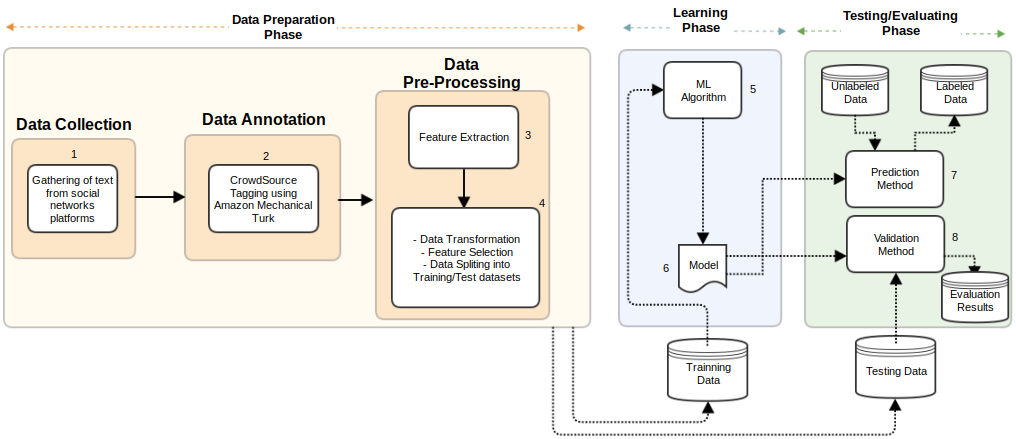
\includegraphics[scale=0.6]{./Figures/system-view/system-overview.png}
  	\rule{24cm}{0.5pt}
	\caption[System Overview]{System Overview}
	\label{fig:system-view}

\end{sidewaysfigure}

In the first stage, data from social networks is collected (1). Well-known platforms like Twitter and Facebook are be the primary sources of social content. The raw social text will then be manually annotated by people using a crowdsourcing technique. In order to achieve this, the documents are manually annotated (2). After this manual process is completed, linguistic features are extracted automatically from the texts (3). There may be data processing afterwards in order to improve the performance of the generated model (4). This stage is very important because it affects directly the performance of the chosen learning algorithm. There is an intermediate stage where a predictive model is generated through a learning algorithm (4, 5). In this case, a supervised model will be trained. NLP features will be used to extract the inputs for the ML algorithm. For instance, we may use probabilistic methods such as Bayesian Networks, search methods such as Decision Trees, optimization methods such as Support Vector Machines or even a model that combines different classifiers. \\
In the next phase, the model is tested against new data and is used to predict new relevant information. Besides, it is also important to evaluate the model using common evaluation metrics, such as precision, recall and F1, in order to extract conclusions about the performance of the model. The feedback obtained in this phase can then be used make improvements in the previous phases.\\
This work focus on the later phases of the process, that is, feature extraction and selection (3, 4), training of a predictive model (5, 6) using linguistic features extracted in the previous phase and testing and evaluation of the created model (7, 8).
The end result is a standalone classifier capable of detecting relevance from documents which might be integrated in a system.  

\section{Dataset}

%Characterization
Our experiments were supported by textual messages gathered from Twitter and Facebook, using their official APIs, in the period between the 16th to the 20th of April, 2016.
It is important to note that, during this process, text quality was preferred over text quantity.

Tweets were retrieved with the following search queries: (i)~``refugees'' and ``Syria''; (ii)~``elections'' and ``US''; (iii)~``Olympic Games''; (iv)~``terrorism''; (v)~``Daesh''; (vi)~``Referendum'' and ``UK'' and ``EU''.
The previous were selected due to their connection with topics currently discussed on the news and social networks.
Retweets were discarded.

Regarding Facebook, posts and comments were gathered from the official pages of several international news websites, namely Euronews, CNN, Washington Post, Financial Times, New York Post, The New York Times, BBC News, The Telegraph, The Guardian, The Huffington Post, Der Spiegel International, Deutsche Welle News, Pravda and Fox News.
While most of the posts would be relevant, comments would contain more diverse information, from this point of view. This would ensure that relevant and irrelevant information was kept.
Also, only documents that met the following conditions were actually used: (i)~between 8 and 100 words; (ii)~written in English; (iii)~not profanity words; (iv)~contained all the words from at least on of the search queries.

In days following their collection, the collected documents were uploaded to the CrowdFlower\footnote{\url{https://www.crowdflower.com/}} platform where an annotation task was launched.
Given a post, volunteer contributors were asked the following questions, using a 5-point Likert scale and regarding journalistic criteria:
(a)~interesting, in opposition to not interesting~(Interest) ; (b)~controversial or not~(Controversy); (c)~meaningful for a general audience in opposition to private/personal (Meaningfulness); (d)~new, in opposition to already known~(Novelty); (e)~reliable or unreliable~(Reliability); (f)~wide or narrow scope (Scope); and (g)~relevant or irrelevant~(Relevance).
To ensure some degree of quality, the texts were classified by at least three different contributors, all of them with the top Crowdflower level~(3), either from USA or UK, in order to control cultural differences. This monitoring was performed another team, belonging to the main project, responsible for the data collection.

%In this phase, we focus on the answers given for the relevance parameter.
To make our task a binary classification problem, each post had to be classified either as relevant or irrelevant.
For that purpose, the median of the answers given by the different contributors was computed and, if it was 4 or 5, the post was considered to be relevant, otherwise, irrelevant. The same method was employed for the others journalistic criteria.
Tables \ref{table-relevance-dataset},\ref{table-interesting-dataset},\ref{table-controversial-dataset},\ref{table-meaningful-dataset},\ref{table-new-dataset},\ref{table-reliable-dataset} details the number of documents grouped by social network, query and label.

%,\ref{table-dataset-fb-comments} and \ref{table-dataset-tweets} details the number of text fragments grouped by social network, search keyword and relevance label.
%Each contributor had to take at least 20 seconds to complete the task.


\begin{table*}[!htpb]
\centering
\footnotesize
\resizebox{\textwidth}{!}{%
\begin{tabular}{|l|l|l|l|l|l|l|}
\hline
\multicolumn{1}{|c|}{}
& \multicolumn{2}{c|}{\textbf{\#Facebook Posts}}
& \multicolumn{2}{c|}{\textbf{\#Facebook Comments}}
& \multicolumn{2}{c|}{\textbf{\#Tweets}} \\ \hline
\textbf{Search Word} & \textbf{Relevant} & \textbf{Irrelevant} & \textbf{Relevant} & \textbf{Irrelevant} & \textbf{Relevant} & \textbf{Irrelevant} \\
\hline
\it ``Refugees'' + ``Syria'' & 20 &  4 & 30 & 13 & 55 & 23 \\
%\hline
\it ``Elections'' + ``US' & 21 & 8 & 21 & 14 & 29 & 39 \\
%\hline
\it ``Olympic Games'' & 2 & 0 & 4 & 1 & 22 & 114 \\
%\hline
\it ``Terrorism'' & 53 & 16 & 138 & 88 & 59 & 53 \\
%\hline
\it ``Daesh'' & 2 & 0 & 14 & 12 & 26 & 30 \\
%\hline
\it ``Referendum'' + ``UK'' + ``EU'' & 4 & 0 & 7 & 1 & 14 & 4 \\
\hline
\end{tabular}%
}
\caption{Documents grouped by source, relevance label and query}
\label{table-relevance-dataset}
\end{table*}

\begin{table*}[!htpb]
\centering
\footnotesize
\resizebox{\textwidth}{!}{%
\begin{tabular}{|l|l|l|l|l|l|l|}
\hline
\multicolumn{1}{|c|}{}
& \multicolumn{2}{c|}{\textbf{\#Facebook Posts}}
& \multicolumn{2}{c|}{\textbf{\#Facebook Comments}}
& \multicolumn{2}{c|}{\textbf{\#Tweets}} \\ \hline
\textbf{Search Word} & \textbf{Interesting} & \textbf{Uninteresting} & \textbf{Interesting} & \textbf{Uninteresting} & \textbf{Interesting} & \textbf{Irrelevant} \\
\hline
\it ``Refugees'' + ``Syria'' & 21 & 3 & 30 & 13 & 55 & 23 \\
%\hline
\it ``Elections'' + ``US' & 17 & 12 & 21 & 14 & 27 & 41 \\
%\hline
\it ``Olympic Games'' & 2 & 0 & 5 & 0 & 21 & 115 \\
%\hline
\it ``Terrorism'' & 57 & 12 & 163 & 63 & 67 & 45 \\
%\hline
\it ``Daesh'' & 2 & 0 & 18 & 8 & 24 & 32 \\
%\hline
\it ``Referendum'' + ``UK'' + ``EU'' & 3 & 1 & 6 & 2 & 13 & 5 \\
\hline
\end{tabular}%
}
\caption{Documents grouped by source, interestingness label and query}
\label{table-interesting-dataset}
\end{table*}

\begin{table*}[!htpb]
\centering
\footnotesize
\resizebox{\textwidth}{!}{%
\begin{tabular}{|l|l|l|l|l|l|l|}
\hline
\multicolumn{1}{|c|}{}
& \multicolumn{2}{c|}{\textbf{\#Facebook Posts}}
& \multicolumn{2}{c|}{\textbf{\#Facebook Comments}}
& \multicolumn{2}{c|}{\textbf{\#Tweets}} \\ \hline
\textbf{Search Word} & \textbf{Controversial} & \textbf{Uncontroversial} & \textbf{Controversial} & \textbf{Uncontroversial} & \textbf{Controversial} & \textbf{Uncontroversial} \\
\hline
\it ``Refugees'' + ``Syria'' & 16 & 8 & 38 & 5 & 53 & 25 \\
%\hline
\it ``Elections'' + ``US' & 10 & 19 & 20 & 15 & 32 & 36 \\
%\hline
\it ``Olympic Games'' & 1 & 1 & 4 & 1 & 9 & 127 \\
%\hline
\it ``Terrorism'' & 44 & 25 & 186 & 40 & 74 & 38 \\
%\hline
\it ``Daesh'' & 2 & 0 & 17 & 9 & 26 & 30 \\
%\hline
\it ``Referendum'' + ``UK'' + ``EU'' & 1 & 3 & 7 & 1 & 9 & 9 \\
\hline
\end{tabular}%
}
\caption{Documents grouped by source, controversialness label and query}
\label{table-controversial-dataset}
\end{table*}

\begin{table*}[!htpb]
\centering
\footnotesize
\resizebox{\textwidth}{!}{%
\begin{tabular}{|l|l|l|l|l|l|l|}
\hline
\multicolumn{1}{|c|}{}
& \multicolumn{2}{c|}{\textbf{\#Facebook Posts}}
& \multicolumn{2}{c|}{\textbf{\#Facebook Comments}}
& \multicolumn{2}{c|}{\textbf{\#Tweets}} \\ \hline
\textbf{Search Word} & \textbf{Meaningful} & \textbf{Meaningless} & \textbf{Meaningful} & \textbf{Meaningless} & \textbf{Meaningful} & \textbf{Meaningless} \\
\hline
\it ``Refugees'' + ``Syria'' & 19 & 5 & 32 & 11 & 56 & 22 \\
%\hline
\it ``Elections'' + ``US' & 25 & 4 & 21 & 14 & 32 & 36 \\
%\hline
\it ``Olympic Games'' & 2 & 0 & 4 & 1 & 36 & 100 \\
%\hline
\it ``Terrorism'' & 59 & 10 & 152 & 74 & 62 & 50 \\
%\hline
\it ``Daesh'' & 2 & 0 & 18 & 8 & 26 & 30 \\
%\hline
\it ``Referendum'' + ``UK'' + ``EU'' & 4 & 0 & 7 & 1 & 15 & 3 \\
\hline
\end{tabular}%
}
\caption{Documents grouped by source, meaningfulness label and query}
\label{table-meaningful-dataset}
\end{table*}

\begin{table*}[!htpb]
\centering
\footnotesize
\resizebox{\textwidth}{!}{%
\begin{tabular}{|l|l|l|l|l|l|l|}
\hline
\multicolumn{1}{|c|}{}
& \multicolumn{2}{c|}{\textbf{\#Facebook Posts}}
& \multicolumn{2}{c|}{\textbf{\#Facebook Comments}}
& \multicolumn{2}{c|}{\textbf{\#Tweets}} \\ \hline
\textbf{Search Word} & \textbf{New} & \textbf{Old} & \textbf{New} & \textbf{Old} & \textbf{New} & \textbf{Old} \\
\hline
\it ``Refugees'' + ``Syria'' & 17 & 7 & 11 & 32 & 38 & 40 \\
%\hline
\it ``Elections'' + ``US' & 12 & 17 & 13 & 22 & 28 & 40 \\
%\hline
\it ``Olympic Games'' & 2 & 0 & 5 & 0 & 54 & 82 \\
%\hline
\it ``Terrorism'' & 32 & 37 & 73 & 153 & 53 & 59 \\
%\hline
\it ``Daesh'' & 1 & 1 & 7 & 19 & 29 & 27 \\
%\hline
\it ``Referendum'' + ``UK'' + ``EU'' & 2 & 2 & 2 & 6 & 12 & 6 \\
\hline
\end{tabular}%
}
\caption{Documents grouped by source, novelty label and query}
\label{table-new-dataset}
\end{table*}

\begin{table*}[!htpb]
\centering
\footnotesize
\resizebox{\textwidth}{!}{%
\begin{tabular}{|l|l|l|l|l|l|l|}
\hline
\multicolumn{1}{|c|}{}
& \multicolumn{2}{c|}{\textbf{\#Facebook Posts}}
& \multicolumn{2}{c|}{\textbf{\#Facebook Comments}}
& \multicolumn{2}{c|}{\textbf{\#Tweets}} \\ \hline
\textbf{Search Word} & \textbf{Reliable} & \textbf{Unreliable} & \textbf{Reliable} & \textbf{Unreliable} & \textbf{Reliable} & \textbf{Unreliable} \\
\hline
\it ``Refugees'' + ``Syria'' & 18 & 6 & 13 & 30 & 40 & 38 \\
%\hline
\it ``Elections'' + ``US' & 14 & 15 & 12 & 23 & 16 & 52 \\
%\hline
\it ``Olympic Games'' & 2 & 0 & 2 & 3 & 43 & 93 \\
%\hline
\it ``Terrorism'' & 41 & 28 & 61 & 165 & 34 & 78 \\
%\hline
\it ``Daesh'' & 1 & 1 & 9 & 17 & 13 & 43 \\
%\hline
\it ``Referendum'' + ``UK'' + ``EU'' & 4 & 0 & 1 & 7 & 10 & 8 \\
\hline
\end{tabular}%
}
\caption{Documents grouped by source, reliability label and query}
\label{table-reliable-dataset}
\end{table*}

\begin{table*}[!htpb]
\centering
\footnotesize
\resizebox{\textwidth}{!}{%
\begin{tabular}{|l|l|l|l|l|l|l|}
\hline
\multicolumn{1}{|c|}{}
& \multicolumn{2}{c|}{\textbf{\#Facebook Posts}}
& \multicolumn{2}{c|}{\textbf{\#Facebook Comments}}
& \multicolumn{2}{c|}{\textbf{\#Tweets}} \\ \hline
\textbf{Search Word} & \textbf{Wide} & \textbf{Narrow} & \textbf{Wide} & \textbf{Narrow} & \textbf{Wide} & \textbf{Narrow} \\
\hline
\it ``Refugees'' + ``Syria'' & 15 & 9 & 21 & 22 & 39 & 39 \\
%\hline
\it ``Elections'' + ``US' & 15 & 14 & 12 & 23 & 16 & 52 \\
%\hline
\it ``Olympic Games'' & 1 & 1 & 4 & 1 & 19 & 117 \\
%\hline
\it ``Terrorism'' & 41 & 28 & 87 & 139 & 41 & 71 \\
%\hline
\it ``Daesh'' & 2 & 0 & 10 & 16 & 15 & 41 \\
%\hline
\it ``Referendum'' + ``UK'' + ``EU'' & 3 & 1 & 0 & 8 & 9 & 9 \\
\hline
\end{tabular}%
}
\caption{Documents grouped by source, scope label and query}
\label{table-scope-dataset}
\end{table*}

In total, the data set contained 130 Facebook posts~(FB post), 343 Facebook comments~(FB comment) and 468 tweets, in a total of 941 instances. Of those, 521 text fragments were annotated as relevant, 420 as irrelevant, 552 as interesting, 389 as uninteresting, 549 as controversial, 392 as uncontroversial, 572 as meaningful, 369 as meaningless, 391 as new, 550 as old, 334 as reliable, 607 as unreliable, 350 as wide and 591 as narrow. \\
Table \ref{tab:text-examples} shows selected messages from the dataset and their source. For the same selected messages, Table~\ref{tab:label-answers} shows the answers on their labels and the resulting class.

\begin{table}[H]
\centering
\footnotesize
\begin{tabular}{|p{7cm}|l|l|}
\hline
\textbf{Content} & \textbf{Source} & \textbf{Post ID}\\
\hline
\scriptsize \it Putin: Turkey supports terrorism and stabs Russia in the back & FB post  & 1
\\
\scriptsize \it Canada to accept additional 10,000 Syrian refugees & Tweet & 2
\\
\scriptsize \it Lololol winning the internet and stomping out daesh \#merica & Tweet &3 
\\
\scriptsize \it Comparing numbers of people killed by terrorism with numbers killed by slipping in bath tub is stupid as eff. It totally ignores the mal-intent behind terrorism, its impact on way of life and ideology. & FB comment & 4
\\
\hline
\end{tabular}
\caption{Examples of messages in the dataset.}
\label{tab:text-examples}
\end{table}

\begin{table}[H]
\small
\centering
\begin{tabular}{|c|c|c|c|c|c|}
\hline
\multirow{2}{*}{\textbf{Criteria}} & \multicolumn{3}{c|}{\textbf{Answers}} & \multirow{2}{*}{\textbf{Class}} &  \multirow{2}{*}{\textbf{Post ID}} \\ \cline{2-4}
 & A1 & A2 & A3 & & \\ \hline
\multirow{4}{*}{Relevance} & 5 & 4 & 5 & Relevant & 1\\ \cline{2-6} 
 & 4 & 5 & 5 & Relevant & 2\\ \cline{2-6} 
 & 1 & 1 & 1 & Irrelevant & 3\\ \cline{2-6} 
 & 2 & 4 & 3 & Irrelevant & 4\\ \hline
 \multirow{4}{*}{Controversialness}  & 4 & 5 & 3 & Controversial & 1\\ \cline{2-6}  
 & 3 & 3 & 4 & Uncontroversial & 2 \\ \cline{2-6} 
 & 1 & 1 & 1 & Uncontroversial & 3\\ \cline{2-6}
 & 2 & 5 & 4 & Controversial & 4\\ \hline
  \multirow{4}{*}{Interestingness}  & 2 & 5 & 4 & Interesting & 1 \\ \cline{2-6} 
 & 4 & 4 & 4 & Interesting & 2\\ \cline{2-6} 
 & 1 & 1 & 1 & Uninteresting & 3\\ \cline{2-6}
 & 2 & 4 & 4 & Interesting & 4\\ \hline
  \multirow{4}{*}{Meaningfulness}  & 3 & 4 & 4 & Meaningful & 1 \\ \cline{2-6} 
 & 4 & 5 & 5 & Meaningful & 2 \\ \cline{2-6} 
 & 2 & 1 & 1 & Meaningless & 3\\ \cline{2-6}
 & 3 & 5 & 4 & Meaningful & 4\\ \hline
  \multirow{4}{*}{Novelty}  & 4 & 2 & 4 & New  & 1\\ \cline{2-6} 
 & 4 & 3 & 4 & New & 2 \\ \cline{2-6} 
 & 2 & 5 & 1 & Old & 3\\ \cline{2-6}
 & 2 & 5 & 3 & Old & 4\\ \hline
  \multirow{4}{*}{Reliability}  & 4 & 3 & 3 & Unreliable & 1 \\ \cline{2-6} 
 & 3 & 5 & 4 & Reliable & 2\\ \cline{2-6} 
 & 1 & 2 & 1 & Unreliable & 3\\ \cline{2-6}
 & 4 & 3 & 3 & Reliable & 4\\ \hline
  \multirow{4}{*}{Scope}  & 4 & 3 & 4 & Wide & 1\\ \cline{2-6} 
 & 2 & 5 & 5 & Wide & 2\\ \cline{2-6} 
 & 1 & 2 & 1 & Narrow & 3 \\ \cline{2-6}
 & 2 & 4 & 3 & Narrow & 4\\ \hline
\end{tabular}	
\caption[Answers on their labels and the resulting class]{Answers on their labels and the resulting class}
\label{tab:label-answers}
\end{table}

\section{Feature Extraction}\label{sec:features}

Our classification model was learned from a set of linguistic features extracted from each message. Initially, those were selected empirically and included: counts of PoS tags, chunk tags, NE tags and 1 to 3-grams of tokens with cutoff frequency~($f$) of 3, i.e., token n-grams that did not appear at least 3 times in the entire corpus were excluded.
We also used 1 to 5 grams of lemmatized tokens (including stopwords and punctuation signs), stems, PoS and chunk tags. Furthermore, we also included simple numerical counts such as the total number of PoS tags, chunk tags, named entities, characters, tokens, all capitalized words and their proportion in the phrase as well.
Finally, we included 3 sentiment features, namely the number of positive and negative words in the message, according to Hu and Liu's Opinion Lexicon\footnote{\url{https://www.cs.uic.edu/~liub/FBS/sentiment-analysis.html\#lexicon}}, which is a manually created lexicon that includes English words with their associated polarity, i.e., according to their perceived opinion (positive or negative). If a word was not there, it was considered to be neutral.
%Additionally, we included a typical bag-of-words in our initial feature set -- each word was treated as an unique feature with the corresponding frequency as the feature value.
Table~\ref{table-features} details the feature sets used and the distinct number of features of each kind. These features are extracted from common NLP tasks presented in section \ref{nlp_tasks} are suitable for text classification tasks\citep{scott1999feature,moschitti2004complex,Biro2008LDASpam,liu2010sentiment}.

\begin{table}[!htpb]
\centering
\footnotesize
\begin{tabular}{|l|l|}
\hline
\textbf{Feature Set} & \textbf{\#Distinct Features} 
\\
\hline
PoS-tags & 54 \\
%\hline
Chunk tags & 23 \\
%\hline
NE tags & 11 \\
%\hline
Total number of PoS/Chunk tags & 2 \\
%\hline
Total number of Named Entities & 1 \\
%\hline
Total number of positive/neutral/negative words & 3 \\
%\hline
Total number of characters/tokens & 2 \\
%\hline
Total number/proportion of all capitalized words & 2 \\
%\hline
LDA topic distribution & 20 \\
%\hline
Token 1-3grams & 2711 ($f \geq 3$ ) \\
%\hline
Lemma 1-5grams & top-750 ($f \geq 1$ ) \\
%\hline
Stem 1-5grams & top-750 ($f \geq 1$ ) \\
%\hline
PoS 1-5grams (1-5) & top-125 ($f \geq 1$ ) \\
%\hline
Chunk 1-5grams (1-5) & top-125 ($f \geq 1$ ) \\
%\hline
%Bag-of-stems & ? ($f\geq3$) \\
\hline
\textbf{Total} & 4,579 \\
%Bag-of-Words & 5,277  \\
\hline
\end{tabular}
\caption[Feature sets used]{Feature sets used}
\label{table-features}
\end{table}  

Naturally, some of the 4,579 distinct features of the initial set do not have enough discriminative power and are not distinguishing or informative enough for the classification task. Therefore, further feature selection/reduction methods should improve the quality of the final predictions.

\section{Baseline Results}
\label{sec:baseline-experiements}

This section describes baseline experiments, for detecting relevance, where we considered different sets of features and did not apply any preprocessing or feature selection method. We started with the full set of features and split the original feature set into smaller ones where only specific features were included. 

Several tools were used in our experiments. NLP features were extracted with the help of TweetNLP~\citep{Gimpel2011TweetNLP}, for PoS tagging, Twitter NLP~\citep{Ritter2011TwitterNLP}, for chunk tagging and NER, both using the pre-trained available models, and NLTK~\citep{Bird2006NLTK} for lemmatisation and stemming. For extracting n-grams, scikit-learn's\footnote{\url{http://scikit-learn.org/stable}} \citep{scikit-learn} tool  was used. Classification experiments were also performed with this machine learning toolkit. Moreover, a GUI application was developed, in Python, using PyQT5\footnote{https://pypi.python.org/pypi/PyQt5}, to aid in the execution of the different steps of the machine learning pipeline such as feature extraction, preprocessing, feature selection/reduction, classification and evaluation.

Tables \ref{tab:baseline-mdc}, \ref{tab:baseline-knn}, \ref{tab:baseline-nb}, \ref{tab:baseline-svm}, \ref{tab:baseline-dt} \ref{tab:baseline-rt} show the results of the different classification methods applied to these smaller subsets of features. Each table presents the obtained results: accuracy, precision, recall, F$_1$-score, area under the ROC curve (AUC) and average precision (AP). The minimum distance and the k-Nearest Neighbors (kNN) classifiers use the Euclidean distance as the distance metric. The number of considered neighbors was 29 since our training data contained a total of 846 instances (90\% of the dataset) and $\sqrt[]{N}$ is usually a good starting point, according to \citep{duda2012pattern}. The SVM classifier uses a linear kernel with the constant $C$ equal to 1 and the Random Forest has a total of 96 trees, which is in the middle of the range [64,128] which provides a good balance between AUC and processing time \citep{Oshiro2012}. Finally, we performed a 10-fold stratified cross validation to obtain the average results and standard deviations. 


\begin{table}[H]
\centering
\small
\resizebox{\textwidth}{!}{%
\begin{tabular}{|l|c|c|c|c|c|c|}
\hline
\multicolumn{1}{|r|}{\textbf{Classifier}} & \multicolumn{6}{c|}{\textbf{Minimum Distance Classifier}} \\ \hline
\multicolumn{1}{|r|}{\textbf{Performance Metrics}} & \multirow{2}{*}{\textbf{Accuracy}} & \multirow{2}{*}{\textbf{Precision}} & \multirow{2}{*}{\textbf{Recall}} & \multirow{2}{*}{\textbf{F$_1$}} & \multirow{2}{*}{\textbf{AP}} & \multirow{2}{*}{\textbf{AUC}} \\ \cline{1-1}
\textbf{Feature Set} &  &  &  &  &  &  \\ \hline
Full feature set &  0.57 $\pm$ 0.05 & \textbf{0.72 $\pm$ 0.14} & 0.41 $\pm$ 0.14 & 0.50 $\pm$ 0.11 & 0.73 $\pm$ 0.07 & 0.59 $\pm$ 0.05 \\ \hline
Part-of-speech & 0.57 $\pm$ 0.06 & 0.71 $\pm$ 0.15 & 0.42 $\pm$ 0.14 & 0.50 $\pm$ 0.11 & 0.72 $\pm$ 0.07 & 0.58 $\pm$ 0.06 \\ \hline
Chunks & 0.57 $\pm$ 0.05 & 0.71 $\pm$ 0.14 & 0.42 $\pm$ 0.13 & 0.51 $\pm$ 0.10 & 0.72 $\pm$ 0.07 & 0.59 $\pm$ 0.05 \\ \hline
Named entities & 0.57 $\pm$ 0.05 & 0.71 $\pm$ 0.14 & 0.42 $\pm$ 0.13 & 0.51 $\pm$ 0.10 & 0.72 $\pm$ 0.07 & 0.58 $\pm$ 0.05 \\ \hline
Chars+Tokens+Allcaps+Allcaps-ratio & 0.57 $\pm$ 0.06 & 0.71 $\pm$ 0.14 & 0.41 $\pm$ 0.14 & 0.50 $\pm$ 0.11 & 0.73 $\pm$ 0.07 & 0.59 $\pm$ 0.05 \\ \hline
Positive+Neutral+Negative & 0.56 $\pm$ 0.05 & 0.70 $\pm$ 0.15 & 0.41 $\pm$ 0.13 & 0.50 $\pm$ 0.11 & 0.72 $\pm$ 0.07 & 0.58 $\pm$ 0.05 \\ \hline
LDA topic distribution & \textbf{0.63 $\pm$ 0.15} & 0.65 $\pm$ 0.17 & \textbf{0.89 $\pm$ 0.17} & \textbf{0.73 $\pm$ 0.12} &\textbf{ 0.80 $\pm$ 0.09} & \textbf{0.60 $\pm$ 0.17} \\ \hline
Token n-grams & 0.57 $\pm$ 0.06 & 0.70 $\pm$ 0.16 & 0.46 $\pm$ 0.15 & 0.53 $\pm$ 0.11 & 0.73 $\pm$ 0.08 & 0.58 $\pm$ 0.06 \\ \hline
Lemma n-grams & 0.58 $\pm$ 0.05 & 0.71 $\pm$ 0.14 & 0.48 $\pm$ 0.15 & 0.55 $\pm$ 0.10 & 0.74 $\pm$ 0.07 & \textbf{0.60 $\pm$ 0.05} \\ \hline
Stem n-grams & 0.59 $\pm$ 0.05 & \textbf{0.72 $\pm$ 0.13} & 0.48 $\pm$ 0.15 & 0.55 $\pm$ 0.10 & 0.74 $\pm$ 0.06 & \textbf{0.60 $\pm$ 0.05} \\ \hline
PoS n-grams & 0.58 $\pm$ 0.05 & 0.71 $\pm$ 0.11 & 0.46 $\pm$ 0.16 & 0.53 $\pm$ 0.12 & 0.73 $\pm$ 0.05 & 0.59 $\pm$ 0.05 \\ \hline
Chunk n-grams & 0.57 $\pm$ 0.06 & 0.70 $\pm$ 0.15 & 0.43 $\pm$ 0.14 & 0.51 $\pm$ 0.11 & 0.72 $\pm$ 0.07 & 0.59 $\pm$ 0.05 \\ \hline
\end{tabular}%
}
\caption[Baseline Results for the Minimum Distance Classifier]{Baseline Results for the Minimum Distance Classifier}
\label{tab:baseline-mdc}
\end{table}

\begin{table}[H]
\centering
\small
\resizebox{\textwidth}{!}{%
\begin{tabular}{|l|c|c|c|c|c|c|}
\hline
\multicolumn{1}{|r|}{\textbf{Classifier}} & \multicolumn{6}{c|}{\textbf{k-Nearest Neighbors (kNN)}} \\ \hline
\multicolumn{1}{|r|}{\textbf{Performance Metrics}} & \multirow{2}{*}{\textbf{Accuracy}} & \multirow{2}{*}{\textbf{Precision}} & \multirow{2}{*}{\textbf{Recall}} & \multirow{2}{*}{\textbf{F$_1$}} & \multirow{2}{*}{\textbf{AP}} & \multirow{2}{*}{\textbf{AUC}} \\ \cline{1-1}
\textbf{Feature Set} &  &  &  &  &  &  \\ \hline
Full feature set & 0.57 $\pm$ 0.05 & 0.60 $\pm$ 0.05 & 0.73$\pm$ 0.12 & 0.65 $\pm$ 0.05 & 0.74 $\pm$ 0.03 & 0.55 $\pm$ 0.06 \\ \hline
Part-of-speech & 0.60 $\pm$ 0.06 & 0.61 $\pm$ 0.05 & 0.83 $\pm$ 0.09 & 0.70 $\pm$ 0.05 & 0.77 $\pm$ 0.03 & 0.58 $\pm$ 0.07 \\ \hline
Chunks & 0.58 $\pm$ 0.04 & 0.58 $\pm$ 0.04 & 0.76 $\pm$ 0.09 & 0.67 $\pm$ 0.04 & 0.75 $\pm$ 0.03 & 0.56 $\pm$ 0.05 \\ \hline
Named entities & 0.58 $\pm$ 0.07 & 0.62 $\pm$ 0.08 & 0.71 $\pm$ 0.11 & 0.65 $\pm$ 0.06 & 0.74 $\pm$ 0.05 & 0.57 $\pm$ 0.08  \\ \hline
Chars+Tokens+Allcaps+Allcaps-ratio & 0.57 $\pm$ 0.06 & 0.60 $\pm$ 0.05 & 0.70 $\pm$ 0.09 & 0.64 $\pm$ 0.05 & 0.73 $\pm$ 0.03 & 0.55 $\pm$ 0.06 \\ \hline
Positive+Neutral+Negative & 0.54 $\pm$ 0.06 & 0.58 $\pm$ 0.04 & 0.62 $\pm$ 0.15 & 0.59 $\pm$ 0.09 & 0.71 $\pm$ 0.05 & 0.53 $\pm$ 0.05 \\ \hline
LDA topic distribution & \textbf{0.62 $\pm$ 0.12} & 0.64 $\pm$ 0.13 & \textbf{0.85 $\pm$ 0.13} & \textbf{0.72 $\pm$ 0.09} & \textbf{0.79 $\pm$ 0.07} & \textbf{0.60 $\pm$ 0.14} \\ \hline
Token n-grams & 0.51 $\pm$ 0.05 & \textbf{0.72 $\pm$ 0.15} & 0.20 $\pm$ 0.09 & 0.30 $\pm$ 0.11 & 0.68 $\pm$ 0.08 & 0.55 $\pm$ 0.04 \\ \hline
Lemma n-grams & 0.59 $\pm$ 0.09 & 0.70 $\pm$ 0.14 & 0.47 $\pm$ 0.12 & 0.55 $\pm$ 0.11 & 0.73 $\pm$ 0.09 & \textbf{0.60 $\pm$ 0.09} \\ \hline
Stem n-grams & 0.57 $\pm$ 0.08 & 0.69 $\pm$ 0.15 & 0.43 $\pm$ 0.13 & 0.52 $\pm$ 0.12 & 0.72 $\pm$ 0.09 & 0.59 $\pm$ 0.08 \\ \hline
PoS n-grams & 0.58 $\pm$ 0.05 & 0.61 $\pm$ 0.05 & 0.61 $\pm$ 0.05 & 0.66 $\pm$ 0.06 & 0.74 $\pm$ 0.04 & 0.56 $\pm$ 0.06 \\ \hline
Chunk n-grams & 0.57 $\pm$ 0.05 & 0.60 $\pm$ 0.04 & 0.67 $\pm$ 0.10 & 0.63 $\pm$ 0.05 & 0.73 $\pm$ 0.03 & 0.55 $\pm$ 0.05 \\ \hline
\end{tabular}%
}
\caption[Baseline Results for the k-Nearest Neighbor Classifier]{Baseline Results for the k-Nearest Neighbor Classifier}
\label{tab:baseline-knn}
\end{table}

\begin{table}[H]
\centering
\small
\resizebox{\textwidth}{!}{%
\begin{tabular}{|l|c|c|c|c|c|c|}
\hline
\multicolumn{1}{|r|}{\textbf{Classifier}} & \multicolumn{6}{c|}{\textbf{Naive Bayes}} \\ \hline
\multicolumn{1}{|r|}{\textbf{Performance Metrics}} & \multirow{2}{*}{\textbf{Accuracy}} & \multirow{2}{*}{\textbf{Precision}} & \multirow{2}{*}{\textbf{Recall}} & \multirow{2}{*}{\textbf{F$_1$}} & \multirow{2}{*}{\textbf{AP}} & \multirow{2}{*}{\textbf{AUC}} \\ \cline{1-1}
\textbf{Feature Set} &  &  &  &  &  &  \\ \hline
Full feature set & 0.60 $\pm$ 0.11 & 0.63 $\pm$ 0.11 & 0.73 $\pm$ 0.16 & 0.66 $\pm$ 0.12 & 0.75 $\pm$ 0.08 & 0.59 $\pm$ 0.12 \\ \hline
Part-of-speech & 0.58 $\pm$ 0.07 & 0.70 $\pm$ 0.13 & 0.33 $\pm$ 0.11 & 0.44 $\pm$ 0.10 & 0.70 $\pm$ 0.07 & 0.57 $\pm$ 0.05 \\ \hline
Chunks & 0.46 $\pm$ 0.03 & 0.50 $\pm$ 0.30 & 0.07 $\pm$ 0.06 & 0.12 $\pm$ 0.09 & 0.64 $\pm$ 0.11 & 0.51 $\pm$ 0.03 \\ \hline
Named entities & 0.58 $\pm$ 0.09 & 0.58 $\pm$ 0.09 & 0.77 $\pm$ 0.11 & 0.67 $\pm$ 0.06 & 0.75 $\pm$ 0.04 & 0.55 $\pm$ 0.10 \\ \hline
Chars+Tokens+Allcaps+Allcaps-ratio & 0.57 $\pm$ 0.04 & 0.57 $\pm$ 0.02 & \textbf{0.93 $\pm$ 0.07} & 0.70 $\pm$ 0.03 & 0.77 $\pm$ 0.02 & 0.53 $\pm$ 0.04 \\ \hline
Positive+Neutral+Negative & 0.55 $\pm$ 0.06 & 0.69 $\pm$ 0.12 & 0.34 $\pm$ 0.12 & 0.44 $\pm$ 0.12 & 0.70 $\pm$ 0.07 & 0.57 $\pm$ 0.05 \\ \hline
LDA topic distribution & \textbf{0.64 $\pm$ 0.13} & 0.67 $\pm$ 0.16 & 0.82 $\pm$ 0.13 & \textbf{0.72 $\pm$ 0.10} & \textbf{0.79 $\pm$ 0.08} & \textbf{0.62 $\pm$ 0.15} \\ \hline
Token n-grams & 0.61 $\pm$ 0.11 & 0.63 $\pm$ 0.11 & 0.71 $\pm$ 0.16 & 0.66 $\pm$ 0.11 & 0.75 $\pm$ 0.08 & 0.59 $\pm$ 0.11 \\ \hline
Lemma n-grams & 0.59 $\pm$ 0.10 & 0.68 $\pm$ 0.15 & 0.54 $\pm$ 0.12 & 0.59 $\pm$ 0.11 & 0.74 $\pm$ 0.08 & 0.60 $\pm$ 0.10 \\ \hline
Stem n-grams & 0.60 $\pm$ 0.09 & 0.68 $\pm$ 0.14 & 0.56 $\pm$ 0.12 & 0.60 $\pm$ 0.11 & 0.74 $\pm$ 0.08 & 0.60 $\pm$ 0.10 \\ \hline
PoS n-grams & 0.58 $\pm$ 0.06 & \textbf{0.70 $\pm$ 0.15} & 0.48 $\pm$ 0.17 & 0.54 $\pm$ 0.12 & 0.74 $\pm$ 0.07 & 0.59 $\pm$ 0.06 \\ \hline
Chunk n-grams & 0.56 $\pm$ 0.05 & 0.69 $\pm$ 0.12 & 0.42 $\pm$ 0.13 & 0.50 $\pm$ 0.10 & 0.71 $\pm$ 0.06 & 0.58 $\pm$ 0.05 \\ \hline
\end{tabular}%
}
\caption[Baseline Results for the Naive Bayes Classifier]{Baseline Results for the Naive Bayes Classifier}
\label{tab:baseline-nb}
\end{table}

\begin{table}[H]
\centering
\small
\resizebox{\textwidth}{!}{%
\begin{tabular}{|l|c|c|c|c|c|c|}
\hline
\multicolumn{1}{|r|}{\textbf{Classifier}} & \multicolumn{6}{c|}{\textbf{Support Vector Machine (SVM)}} \\ \hline
\multicolumn{1}{|r|}{\textbf{Performance Metrics}} & \multirow{2}{*}{\textbf{Accuracy}} & \multirow{2}{*}{\textbf{Precision}} & \multirow{2}{*}{\textbf{Recall}} & \multirow{2}{*}{\textbf{F$_1$}} & \multirow{2}{*}{\textbf{AP}} & \multirow{2}{*}{\textbf{AUC}} \\ \cline{1-1}
\textbf{Feature Set} &  &  &  &  &  &  \\ \hline
Full feature set & 0.60 $\pm$ 0.10 & \textbf{0.67 $\pm$ 0.14} & 0.63 $\pm$ 0.08 & 0.64 $\pm$ 0.08 & 0.75 $\pm$ 0.07 & 0.60 $\pm$ 0.11 \\ \hline
Part-of-speech & 0.63 $\pm$ 0.08 & 0.66 $\pm$ 0.09 & 0.71 $\pm$ 0.21 & 0.66 $\pm$ 0.12 & 0.76 $\pm$ 0.06 & \textbf{0.62 $\pm$ 0.08} \\ \hline
Chunks & 0.58 $\pm$ 0.07 & 0.59 $\pm$ 0.05 & 0.75 $\pm$ 0.24 & 0.64 $\pm$ 0.15 & 0.64 $\pm$ 0.15 & 0.56 $\pm$ 0.06 \\ \hline
Named entities & 0.55 $\pm$ 0.09 & 0.51 $\pm$ 0.29 & 0.64 $\pm$ 0.42 & 0.51 $\pm$ 0.32 & 0.78 $\pm$ 0.03 & 0.54 $\pm$ 0.07 \\ \hline
Chars+Tokens+Allcaps+Allcaps-ratio & 0.54 $\pm$ 0.06 & 0.45 $\pm$ 0.23 & 0.74 $\pm$ 0.38 & 0.56 $\pm$ 0.28 & 0.77 $\pm$ 0.02 & 0.51 $\pm$ 0.04 \\ \hline
Positive+Neutral+Negative & 0.52 $\pm$ 0.05 & 0.59 $\pm$ 0.26 & 0.60 $\pm$ 0.40 & 0.48 $\pm$ 0.29 & 0.71 $\pm$ 0.15 & 0.51 $\pm$ 0.02 \\ \hline
LDA topic distribution & \textbf{0.64 $\pm$ 0.14} & 0.65 $\pm$ 0.16 & \textbf{0.85 $\pm$ 0.19} & \textbf{0.72 $\pm$ 0.13} & \textbf{0.79 $\pm$ 0.09} & 0.61 $\pm$ 0.16 \\ \hline
Token n-grams & 0.60 $\pm$ 0.09 & 0.65 $\pm$ 0.11 & 0.62 $\pm$ 0.11 & 0.63 $\pm$ 0.09 & 0.74 $\pm$ 0.06 & 0.59 $\pm$ 0.09 \\ \hline
Lemma n-grams & 0.59 $\pm$ 0.07 & 0.65 $\pm$ 0.11 & 0.61 $\pm$ 0.08 & 0.62 $\pm$ 0.06 & 0.74 $\pm$ 0.05 & 0.58 $\pm$ 0.08 \\ \hline
Stem n-grams & 0.61 $\pm$ 0.09 & 0.69 $\pm$ 0.14 & 0.62 $\pm$ 0.11 & 0.64 $\pm$ 0.08 & 0.76 $\pm$ 0.07 & 0.61 $\pm$ 0.09 \\ \hline
PoS n-grams & 0.58 $\pm$ 0.09 & 0.63 $\pm$ 0.12 & 0.63 $\pm$ 0.15 & 0.62 $\pm$ 0.11 & 0.73 $\pm$ 0.08 & 0.58 $\pm$ 0.10 \\ \hline
Chunk n-grams & 0.56 $\pm$ 0.06 & 0.59 $\pm$ 0.05 & 0.69 $\pm$ 0.17 & 0.62 $\pm$ 0.09 & 0.72 $\pm$ 0.05 & 0.54 $\pm$ 0.05 \\ \hline
\end{tabular}%
}
\caption[Baseline Results for the Support Vector Machine Classifier ]{Baseline Results for the Support Vector Machine Classifier}
\label{tab:baseline-svm}
\end{table}

\begin{table}[H]
\centering
\small
\resizebox{\textwidth}{!}{%
\begin{tabular}{|l|c|c|c|c|c|c|}
\hline
\multicolumn{1}{|r|}{\textbf{Classifier}} & \multicolumn{6}{c|}{\textbf{Decision Tree}} \\ \hline
\multicolumn{1}{|r|}{\textbf{Performance Metrics}} & \multirow{2}{*}{\textbf{Accuracy}} & \multirow{2}{*}{\textbf{Precision}} & \multirow{2}{*}{\textbf{Recall}} & \multirow{2}{*}{\textbf{F$_1$}} & \multirow{2}{*}{\textbf{AP}} & \multirow{2}{*}{\textbf{AUC}} \\ \cline{1-1}
\textbf{Feature Set} &  &  &  &  &  &  \\ \hline
Full feature set & 0.58 $\pm$ 0.05 & 0.63 $\pm$ 0.08 & \textbf{0.63 $\pm$ 0.09} & 0.62 $\pm$ 0.05 & 0.73 $\pm$ 0.04 & 0.57 $\pm$ 0.06  \\ \hline
Part-of-speech & 0.57 $\pm$ 0.08 & 0.62 $\pm$ 0.09 & 0.60 $\pm$ 0.06 & 0.61 $\pm$ 0.05 & 0.72 $\pm$ 0.05 & 0.56 $\pm$ 0.08 \\ \hline
Chunks & 0.55 $\pm$ 0.04 & 0.59 $\pm$ 0.04 & 0.59 $\pm$ 0.06 & 0.59 $\pm$ 0.04 & 0.71 $\pm$ 0.03 & 0.54 $\pm$ 0.04 \\ \hline
Named entities & 0.53 $\pm$ 0.04 & 0.58 $\pm$ 0.04 &  0.55 $\pm$ 0.05 & 0.57 $\pm$ 0.04 & 0.69 $\pm$ 0.02 & 0.53 $\pm$ 0.04 \\ \hline
Chars+Tokens+Allcaps+Allcaps-ratio & 0.55 $\pm$ 0.04 & 0.59 $\pm$ 0.04 & 0.61 $\pm$ 0.07 & 0.60 $\pm$ 0.05 & 0.71 $\pm$ 0.03 & 0.54 $\pm$ 0.04 \\ \hline
Positive+Neutral+Negative & 0.53 $\pm$ 0.04 & 0.58 $\pm$ 0.04 & 0.51 $\pm$ 0.10 & 0.54 $\pm$ 0.07 & 0.68 $\pm$ 0.04 & 0.53 $\pm$ 0.04 \\ \hline
LDA topic distribution & 0.55 $\pm$ 0.07 & 0.60 $\pm$ 0.09 & 0.58 $\pm$ 0.08 & 0.59 $\pm$ 0.06 & 0.71 $\pm$ 0.05 & 0.54 $\pm$ 0.08 \\ \hline
Token n-grams & 0.55 $\pm$ 0.12 & 0.61 $\pm$ 0.14 & 0.61 $\pm$ 0.13 & 0.60 $\pm$ 0.11 & 0.72 $\pm$ 0.08 & 0.54 $\pm$ 0.13 \\ \hline
Lemma n-grams & 0.57 $\pm$ 0.10 & 0.63 $\pm$ 0.13 & 0.61 $\pm$ 0.11 & 0.61 $\pm$ 0.09 & 0.73 $\pm$ 0.08 & 0.57 $\pm$ 0.10 \\ \hline
Stem n-grams & 0.56 $\pm$ 0.08 & 0.62 $\pm$ 0.12 & 0.58 $\pm$ 0.10 & 0.59 $\pm$ 0.07 & 0.72 $\pm$ 0.06 &  0.55 $\pm$ 0.08\\ \hline
PoS n-grams & \textbf{0.60 $\pm$ 0.06} & \textbf{0.64 $\pm$ 0.06} & 0.62 $\pm$ 0.08 & \textbf{0.63 $\pm$ 0.06} & \textbf{0.74 $\pm$ 0.04} & \textbf{0.59 $\pm$ 0.06} \\ \hline
Chunk n-grams & 0.56 $\pm$ 0.06 & 0.61 $\pm$ 0.06 & 0.59 $\pm$ 0.08 & 0.60 $\pm$ 0.06 & 0.71 $\pm$ 0.04 & 0.56 $\pm$ 0.06
 \\ \hline
\end{tabular}%
}
\caption[Baseline Results for the Decision Tree Classifier]{Baseline Results for the Decision Tree Distance Classifier}
\label{tab:baseline-dt}
\end{table}

\begin{table}[H]
\centering
\small
\resizebox{\textwidth}{!}{%
\begin{tabular}{|l|c|c|c|c|c|c|}
\hline
\multicolumn{1}{|r|}{\textbf{Classifier}} & \multicolumn{6}{c|}{\textbf{Random Forest Classifier }} \\ \hline
\multicolumn{1}{|r|}{\textbf{Performance Metrics}} & \multirow{2}{*}{\textbf{Accuracy}} & \multirow{2}{*}{\textbf{Precision}} & \multirow{2}{*}{\textbf{Recall}} & \multirow{2}{*}{\textbf{F$_1$}} & \multirow{2}{*}{\textbf{AP}} & \multirow{2}{*}{\textbf{AUC}} \\ \cline{1-1}
\textbf{Feature Set} &  &  &  &  &  &  \\ \hline
Full feature set & \textbf{0.64 $\pm$ 0.06} & 0.66 $\pm$ 0.09 & \textbf{0.78 $\pm$ 0.10} & \textbf{0.71 $\pm$ 0.04} & 0.78 $\pm$ 0.04 & \textbf{0.62 $\pm$ 0.09} \\ \hline
Part-of-speech & 0.63 $\pm$ 0.07 & 0.66 $\pm$ 0.09 & \textbf{0.78 $\pm$ 0.11} & 0.70 $\pm$ 0.05 & 0.78 $\pm$ 0.04 & \textbf{0.62 $\pm$ 0.08} \\ \hline
Chunks & 0.60 $\pm$ 0.04 & 0.62 $\pm$ 0.04 & 0.70 $\pm$ 0.07 & 0.66 $\pm$ 0.04 & 0.74 $\pm$ 0.02 & 0.58 $\pm$ 0.04 \\ \hline
Named entities & 0.58 $\pm$ 0.06 & 0.62 $\pm$ 0.06 & 0.66 $\pm$ 0.07 & 0.64 $\pm$ 0.05 & 0.73 $\pm$ 0.04 & 0.56 $\pm$ 0.06 \\ \hline
Chars+Tokens+Allcaps+Allcaps-ratio & 0.55 $\pm$ 0.03 & 0.59 $\pm$ 0.03 & 0.61 $\pm$ 0.09 & 0.60 $\pm$ 0.05 & 0.71 $\pm$ 0.03 & 0.54 $\pm$ 0.03 \\ \hline
Positive+Neutral+Negative & 0.52 $\pm$ 0.04 & 0.57 $\pm$ 0.03 & 0.57 $\pm$ 0.09 & 0.57 $\pm$ 0.05 & 0.69 $\pm$ 0.03 & 0.51 $\pm$ 0.04 \\ \hline
LDA topic distribution & 0.60 $\pm$ 0.11 & 0.65 $\pm$ 0.16 & 0.75 $\pm$ 0.15 & 0.67 $\pm$ 0.10 & 0.77 $\pm$ 0.08 & 0.58 $\pm$ 0.13	 \\ \hline
Token n-grams & 0.62 $\pm$ 0.10 & 0.66 $\pm$ 0.15 & 0.77 $\pm$ 0.16 & 0.69 $\pm$ 0.09 & 0.78 $\pm$ 0.07 & 0.60 $\pm$ 0.12 \\ \hline
Lemma n-grams & 0.63 $\pm$ 0.11 & 0.66 $\pm$ 0.16 & \textbf{0.78 $\pm$ 0.13} & 0.70 $\pm$ 0.09 & 0.78 $\pm$ 0.08 & 0.61 $\pm$ 0.13 \\ \hline
Stem n-grams & 0.64 $\pm$ 0.11 & \textbf{0.67 $\pm$ 0.15} & 0.78 $\pm$ 0.16 & 0.70 $\pm$ 0.10 & \textbf{0.79 $\pm$ 0.08} & \textbf{0.62 $\pm$ 0.12} \\ \hline
PoS n-grams & 0.62 +- 0.06 & 0.65 +- 0.10 & 0.77 +- 0.11 & 0.69 +- 0.04 & 0.77 +- 0.04 & 0.61 +- 0.08 \\ \hline
Chunk n-grams & 0.59 $\pm$ 0.04 & 0.59 $\pm$ 0.04 & 0.72 $\pm$ 0.10 & 0.66 $\pm$ 0.05 & 0.74 $\pm$ 0.03 & 0.57 $\pm$ 0.05 \\ \hline
\end{tabular}%
}
\caption[Baseline Results for the Random Forest Classifier]{Baseline Results for the Random Forest Classifier}
\label{tab:baseline-rt}
\end{table}

% Considering the full feature set, the Random Forest obtained the best accuracy(0.64). Surprisingly, the Minimum Distance Classifier obtained the best precision(0.72). The Random Forest got the best recall(0.78) while the kNN got the best F$_1$(0.66). The Random Forest obtained the best areas under the roc and precision-recall curves, obtaining (0.75) and (0.62), respectively, closely followed by the SVM classifier.

% Regarding the PoS tags, both SVM and Random Forest obtained an accuracy of 0.63, while the Minimum Distance Classifier got a precision of 0.71  and the kNN got the best recall(0.83). In respect to the F$1$ measure, both kNN and Random Forest obtained 0.70. The SVM classifier achieved the same result as the Random Forest regarding average precision(0.62) while the Random Forest obtained the best AUC(0.78).

The Naive Bayes and the SVM classier achieve the best accuracy(0.64) on the set consisting of LDA topics. The Minimum Distance Classifier obtained the best precisions(0.72) using the full dataset and n-grams of stems while the kNN classifier achieved also the same precision(0.72) using ngams of tokens. The LDA topic distribution proved to be a good feature set, achieving the best recall(0.89), F$_1$ score(0.73) and average precision(0.80) using a Minimum Distance Classifier. In fact, it is possible that some topic distributions were more likely to be associated with relevant data (or irrelevant) and be highly influenced by some typical words. However, the Naive Bayes, the SVM and the Random Forest obtained the best area under the ROC curve(0.62). To achieve this AUC, the Naive Bayes used the LDA topics, the SVM used the PoS tags and the Random Forest achieved the same result by using the full feature set, PoS tags and stem ngrams. 
Surprisingly, for such a simple model such as the Minimum Distance Classifier, it got fairly good results, suggesting that the distance between mean feature vectors is large enough to discriminate both classes. The Random Forest, kNN and the Naive Bayes always competed against the best results, while the Decision Tree did not performed so well, achieving results just a little above a random classifier. Another important note is that small subsets such as the countings of characters/tokens/allcaps/allcaps-ratio (4 features) were sometimes enough to make decent predictions. For example, using this small set, the Naive Bayes achieved a F$_1$ score of 0.70. On the other, the polarity set did not performed very well.  Although some feature sets work better in some cases and worse in others, this suggest that a combination of the most informative features from each set may improve the classification results. 

\begin{figure}[H]
	\centering
	\resizebox{\textwidth}{!}{
  	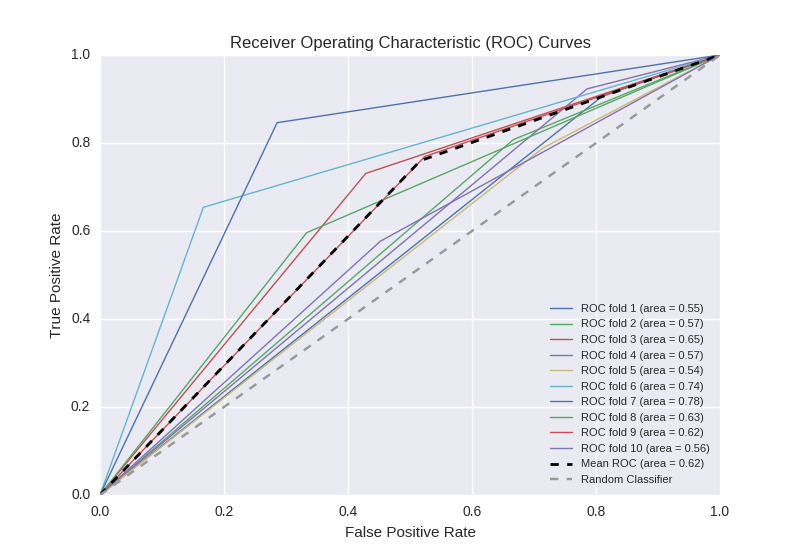
\includegraphics{./Figures/experiments/baseline/roc}
     }
	\caption[ROC Curves of a SVM  Classifier using PoS tags as features]{ROC Curves of a SVM  Classifier using PoS tags as features}
	\label{fig:baseline-roc-svm-pos}
\end{figure}

\begin{figure}[H]
	\centering
	\resizebox{\textwidth}{!}{
  	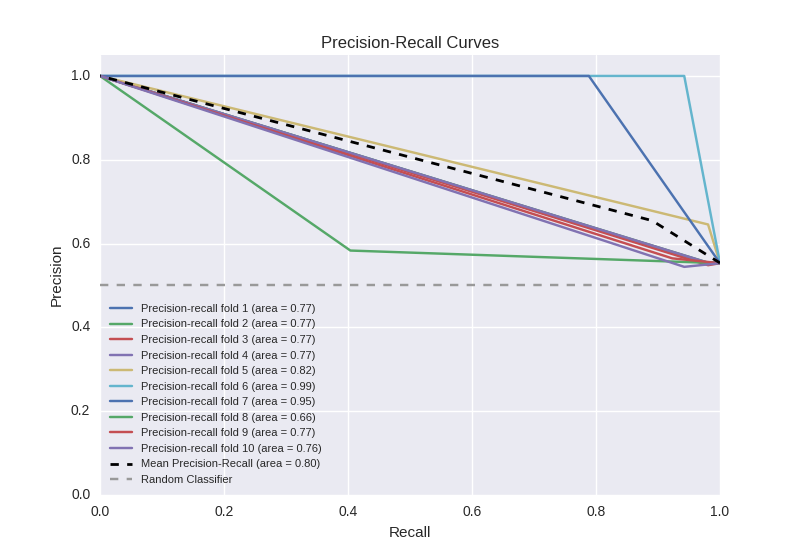
\includegraphics{./Figures/experiments/baseline/pr_curve}
     }
	\caption[Precision-Recall Curves of a Minimum Distance Classifier using LDA topic distributions as features]{Precision-Recall Curves of a Minimum Distance Classifier using LDA topic distributions as features}
	\label{fig:baseline-pr-mdc-lda}
\end{figure}

Figure \ref{fig:baseline-roc-svm-pos} shows the best average ROC curve obtained by a SVM classifier. For low false positive rates ($<$ 0.20), the SVM classifier achieves true positive rates a little better random. However, if we are allowed to increase the false positive rate, the the number of correctly identified instances increases, achieving true positive rates $>$ 0.80 in some cases. Figure \ref{fig:baseline-pr-mdc-lda} shows the best average Precision-Recall curves obtained by a Minimum Distance Classifier. It consistently shows fairy good trade-offs between the obtained precision and recall values, achieving areas greater than $0.90$ in some cases. 



%%%%%%%%%%%%%%%%%%%%%%%%%%%%%%%%%%%%%%%%%%%%%%%%%%%%%%%%%%%%%%%%%%%%%%%%%%%%%%%%%%%%%%%%%%%%%%%%%%%%%%%%%%%%%%%%%%
\section{Feature Engineering Results}
\label{sec:feature-engineering}

Successful removal of noisy and redundant data typically improves the overall classification accuracy of the resulting model, reducing also overfitting. For this purpose, we used different preprocessing methods such as: Standardization, Normalization and Scaling and feature selection methods such as: information gain, gain ratio, chi-square ($\chi^2$), Fisher Score, Pearson correlations and feature reduction techniques such as principal component analysis. The PCA method was applied to 4 dimensions and the Pearson correlations were used to exclude features that did not have a correlation of at least $0.2$ with the target class. The classifiers were used with the same parameterization of the baseline experiments. The 10-fold cross validation was performed as well, where the feature selection/reduction methods were performed within each fold, using only the training set, in order to avoid the feature selection methods using information from the test set, such as labels, and thus avoiding bias. \\
In order to choose the number $f$ of features we followed a very simple heuristic. We applied the $\chi^2$ statistic test to find the number of statistically significant features, i.e., features that had a statistic score of $\chi^2 > 10.83$, meaning that they are very likely to be dependent from the target class, with only a $0.001$ chance of being wrong. The obtained size was $f = 210$ and it was the number of selected features. Tables \ref{tab:fe-mdc},\ref{tab:fe-knn},\ref{tab:fe-nb},\ref{tab:fe-svm},\ref{tab:fe-dt} and \ref{tab:fe-rt} show the obtained results for each classifier in predicting relevance.

\begin{table}[H]
\centering
\small
\resizebox{\textwidth}{!}{%
\begin{tabular}{|l|c|c|c|c|c|c|}
\hline
\multicolumn{1}{|r|}{\textbf{Classifier}} & \multicolumn{6}{c|}{\textbf{Minimum Distance Classifier }} \\ \hline
\multicolumn{1}{|r|}{\textbf{Performance Metrics}} & \multirow{2}{*}{\textbf{Accuracy}} & \multirow{2}{*}{\textbf{Precision}} & \multirow{2}{*}{\textbf{Recall}} & \multirow{2}{*}{\textbf{F$_1$}} & \multirow{2}{*}{\textbf{AP}} & \multirow{2}{*}{\textbf{AUC}} \\ \cline{1-1}
\textbf{Pipeline applied} &  &  &  &  &  &  \\ \hline
Standardization + full feature set & 0.57 $\pm$ 0.05 & \textbf{0.72 $\pm$ 0.14} & 0.41 $\pm$ 0.14 & 0.50 $\pm$ 0.11 & 0.73 $\pm$ 0.07 & 0.59 $\pm$ 0.05 \\ \hline
Normalization + full feature set & 0.57 $\pm$ 0.05 & \textbf{0.72 $\pm$ 0.14} & 0.41 $\pm$ 0.14 & 0.50 $\pm$ 0.11 & 0.73 $\pm$ 0.07 & 0.59 $\pm$ 0.05 \\ \hline
Scaling[0,1] + full feature set & 0.57 $\pm$ 0.05 & \textbf{0.72 $\pm$ 0.14} & 0.41 $\pm$ 0.14 & 0.50 $\pm$ 0.11 & 0.73 $\pm$ 0.07 & 0.59 $\pm$ 0.05 \\ \hline
Standardization + information gain& 0.57 $\pm$ 0.05 & \textbf{0.72 $\pm$ 0.14} & 0.41 $\pm$ 0.14 & 0.50 $\pm$ 0.11 & 0.73 $\pm$ 0.07 & 0.59 $\pm$ 0.05 \\ \hline
Standardization + gain ratio& 0.57 $\pm$ 0.05 & 0.58 $\pm$ 0.06 & \textbf{0.86 $\pm$ 0.17} & \textbf{0.68 $\pm$ 0.05} & \textbf{0.76 $\pm$ 0.04} & 0.53 $\pm$ 0.07 \\ \hline
Standardization + chi square ($\chi^2$)& 0.57 $\pm$ 0.05 & \textbf{0.72 $\pm$ 0.14} & 0.41 $\pm$ 0.14 & 0.50 $\pm$ 0.11 & 0.73 $\pm$ 0.07 & 0.59 $\pm$ 0.05 \\ \hline
Standardization + fisher score& 0.51 $\pm$ 0.07 & 0.62 $\pm$ 0.17 & 0.32 $\pm$ 0.13 & 0.41 $\pm$ 0.11 & 0.66 $\pm$ 0.09 & 0.53 $\pm$ 0.08 \\ \hline
Standardization + pearson & \textbf{0.65 $\pm$ 0.16} & 0.70 $\pm$ 0.15 & 0.63 $\pm$ 0.20 & 0.65 $\pm$ 0.18 & 0.77 $\pm$ 0.11 & \textbf{0.62 $\pm$ 0.16} \\ \hline
Standardization + pearson + pca4d& \textbf{0.65 $\pm$ 0.16} & 0.70 $\pm$ 0.15 & 0.63 $\pm$ 0.20 & 0.65 $\pm$ 0.18 & 0.77 $\pm$ 0.11 & \textbf{0.62 $\pm$ 0.16} \\ \hline
Standardization + gain ratio + pca4d & 0.57 $\pm$ 0.07 & 0.55 $\pm$ 0.08 &\textbf{0.86 $\pm$ 0.29} & 0.65 $\pm$ 0.19 & 0.75 $\pm$ 0.10 & 0.53 $\pm$ 0.06 \\ \hline
\end{tabular}%
}
\caption[Results of applying different Preprocessing and Feature Selection methods with a Minimum Distance Classifier]{Results of applying different Preprocessing and Feature Selection methods with a Minimum Distance Classifier}
\label{tab:fe-mdc}
\end{table}

\begin{table}[H]
\centering
\small
\resizebox{\textwidth}{!}{%
\begin{tabular}{|l|c|c|c|c|c|c|}
\hline
\multicolumn{1}{|r|}{\textbf{Classifier}} & \multicolumn{6}{c|}{\textbf{k-Nearest Neighbors (kNN)}} \\ \hline
\multicolumn{1}{|r|}{\textbf{Performance Metrics}} & \multirow{2}{*}{\textbf{Accuracy}} & \multirow{2}{*}{\textbf{Precision}} & \multirow{2}{*}{\textbf{Recall}} & \multirow{2}{*}{\textbf{F$_1$}} & \multirow{2}{*}{\textbf{AP}} & \multirow{2}{*}{\textbf{AUC}} \\ \cline{1-1}
\textbf{Pipeline applied} &  &  &  &  &  &  \\ \hline
Standardization + full feature set & 0.57 $\pm$ 0.05 & 0.60 $\pm$ 0.05 & 0.73 $\pm$ 0.12 & 0.65 $\pm$ 0.05 & 0.74 $\pm$ 0.03 & 0.55 $\pm$ 0.06 \\ \hline
Normalization + full feature set & 0.57 $\pm$ 0.05 & 0.60 $\pm$ 0.05 & 0.73 $\pm$ 0.12 & 0.65 $\pm$ 0.05 & 0.74 $\pm$ 0.03 & 0.55 $\pm$ 0.06 \\ \hline
Scaling[0,1] + full feature set & 0.57 $\pm$ 0.05 & 0.60 $\pm$ 0.05 & 0.73 $\pm$ 0.12 & 0.65 $\pm$ 0.05 & 0.74 $\pm$ 0.03 & 0.55 $\pm$ 0.06 \\ \hline
Standardization + information gain& 0.58 $\pm$ 0.05 & 0.61 $\pm$ 0.05 & 0.75 $\pm$ 0.11 & 0.66 $\pm$ 0.04 & 0.75 $\pm$ 0.03 & 0.56 $\pm$ 0.05 \\ \hline
Standardization + gain ratio& 0.59 $\pm$ 0.06 & 0.59 $\pm$ 0.06 & \textbf{0.95 $\pm$ 0.11} & 0.72 $\pm$ 0.04 & 0.78 $\pm$ 0.03 & 0.55 $\pm$ 0.08 \\ \hline
Standardization + chi square ($\chi^2$)& 0.57 $\pm$ 0.04 & 0.60 $\pm$ 0.05 & 0.75 $\pm$ 0.11 & 0.66 $\pm$ 0.04 & 0.74 $\pm$ 0.03 & 0.55 $\pm$ 0.05 \\ \hline
Standardization + fisher score& 0.48 $\pm$ 0.06 & 0.58 $\pm$ 0.14 & 0.25 $\pm$ 0.16 & 0.33 $\pm$ 0.14 & 0.62 $\pm$ 0.09 & 0.51 $\pm$ 0.05 \\ \hline
Standardization + pearson & 0.62 $\pm$ 0.13 & 0.62 $\pm$ 0.13 & 0.87 $\pm$ 0.12 & 0.72 $\pm$ 0.10 & 0.78 $\pm$ 0.08 & 0.59 $\pm$ 0.14 \\ \hline
Standardization + pearson + pca4d& \textbf{0.65 $\pm$ 0.15} & \textbf{0.67 $\pm$ 0.17}	 & 0.85 $\pm$ 0.11 & \textbf{0.74 $\pm$ 0.11} & \textbf{	0.80 $\pm$ 0.09} & \textbf{0.63 $\pm$ 0.16} \\ \hline
Standardization + gain ratio + pca4d & 0.54 $\pm$ 0.06 & 0.58 $\pm$ 0.05 & 0.66 $\pm$ 0.10 & 0.61 $\pm$ 0.06 & 0.71 $\pm$ 0.04 & 0.53 $\pm$ 0.06 \\ \hline
\end{tabular}%
}
\caption[Results of applying different Preprocessing and Feature Selection methods with a k-Nearest Neighbors]{Results of applying different Preprocessing and Feature Selection methods with a k-Nearest Neighbors}
\label{tab:fe-knn}
\end{table}

\begin{table}[H]
\centering
\small
\resizebox{\textwidth}{!}{%
\begin{tabular}{|l|c|c|c|c|c|c|}
\hline
\multicolumn{1}{|r|}{\textbf{Classifier}} & \multicolumn{6}{c|}{\textbf{Naive Bayes }} \\ \hline
\multicolumn{1}{|r|}{\textbf{Performance Metrics}} & \multirow{2}{*}{\textbf{Accuracy}} & \multirow{2}{*}{\textbf{Precision}} & \multirow{2}{*}{\textbf{Recall}} & \multirow{2}{*}{\textbf{F$_1$}} & \multirow{2}{*}{\textbf{AP}} & \multirow{2}{*}{\textbf{AUC}} \\ \cline{1-1}
\textbf{Pipeline applied} &  &  &  &  &  &  \\ \hline
Standardization + full feature set & 0.60 $\pm$ 0.11 & 0.63 $\pm$ 0.11 & 0.73 $\pm$ 0.16 & 0.66 $\pm$ 0.12 & 0.75 $\pm$ 0.08 & 0.59 $\pm$ 0.12 \\ \hline
Normalization + full feature set & 0.60 $\pm$ 0.11 & 0.63 $\pm$ 0.11 & 0.73 $\pm$ 0.16 & 0.66 $\pm$ 0.12 & 0.75 $\pm$ 0.08 & 0.59 $\pm$ 0.12 \\ \hline
Scaling[0,1] + full feature set & 0.60 $\pm$ 0.11 & 0.63 $\pm$ 0.11 & 0.73 $\pm$ 0.16 & 0.66 $\pm$ 0.12 & 0.75 $\pm$ 0.08 & 0.59 $\pm$ 0.12 \\ \hline
Standardization + information gain& 0.55 $\pm$ 0.08 & 0.67 $\pm$ 0.14 & 0.41 $\pm$ 0.17 & 0.48 $\pm$ 0.14 & 0.71 $\pm$ 0.08 & 0.57 $\pm$ 0.08 \\ \hline
Standardization + gain ratio& 0.53 $\pm$ 0.06 & 0.57 $\pm$ 0.07 & 0.63 $\pm$ 0.11 & 0.59 $\pm$ 0.06 & 0.70 $\pm$ 0.04 & 0.51 $\pm$ 0.07 \\ \hline
Standardization + chi square ($\chi^2$)& 0.55 $\pm$ 0.06 & 0.67 $\pm$ 0.14 & 0.43 $\pm$ 0.15 & 0.50 $\pm$ 0.11 & 0.71 $\pm$ 0.07 & 0.57 $\pm$ 0.06 \\ \hline
Standardization + fisher score& 0.50 $\pm$ 0.07 & 0.61 $\pm$ 0.16 & 0.27 $\pm$ 0.09 & 0.37 $\pm$ 0.11 & 0.64 $\pm$ 0.09 & 0.52 $\pm$ 0.07 \\ \hline
Standardization + pearson & \textbf{0.65 $\pm$ 0.16} & \textbf{0.66 $\pm$ 0.17} & \textbf{0.94 $\pm$ 0.11} & \textbf{0.76 $\pm$ 0.10} & \textbf{0.82 $\pm$ 0.09} & \textbf{0.61 $\pm$ 0.18} \\ \hline
Standardization + pearson + pca4d& \textbf{0.65 $\pm$ 0.16} & \textbf{0.66 $\pm$ 0.17} & \textbf{0.94 $\pm$ 0.11} & \textbf{0.76 $\pm$ 0.10} & 0.81 $\pm$ 0.09 & \textbf{0.61 $\pm$ 0.18} \\ \hline
Standardization + gain ratio + pca4d & 0.58 $\pm$ 0.05 & 0.58 $\pm$ 0.03 & 0.95 $\pm$ 0.10 & 0.95 $\pm$ 0.10 & 0.78 $\pm$ 0.02 & 0.54 $\pm$ 0.05 \\ \hline
\end{tabular}%
}
\caption[Results of applying different Preprocessing and Feature Selection methods with a Naive Bayes]{Results of applying different Preprocessing and Feature Selection methods with a Naive Bayes}
\label{tab:fe-nb}
\end{table}

\begin{table}[H]
\centering
\small
\resizebox{\textwidth}{!}{%
\begin{tabular}{|l|c|c|c|c|c|c|}
\hline
\multicolumn{1}{|r|}{\textbf{Classifier}} & \multicolumn{6}{c|}{\textbf{Support Vector Machine (SVM)}} \\ \hline
\multicolumn{1}{|r|}{\textbf{Performance Metrics}} & \multirow{2}{*}{\textbf{Accuracy}} & \multirow{2}{*}{\textbf{Precision}} & \multirow{2}{*}{\textbf{Recall}} & \multirow{2}{*}{\textbf{F$_1$}} & \multirow{2}{*}{\textbf{AP}} & \multirow{2}{*}{\textbf{AUC}} \\ \cline{1-1}
\textbf{Pipeline applied} &  &  &  &  &  &  \\ \hline
Standardization + full feature set & 0.58 $\pm$ 0.12 & 0.65 $\pm$ 0.14 & 0.57 $\pm$ 0.21 & 0.58 $\pm$ 0.17 & 0.73 $\pm$ 0.10 & 0.58 $\pm$ 0.12 \\ \hline
Normalization + full feature set & 0.58 $\pm$ 0.09 & 0.66 $\pm$ 0.13 & 0.58 $\pm$ 0.16 & 0.60 $\pm$ 0.10 & 0.74 $\pm$ 0.07 & 0.59 $\pm$ 0.10 \\ \hline
Scaling[0,1] + full feature set & 0.59 $\pm$ 0.11 & 0.65 $\pm$ 0.15 & 0.61 $\pm$ 0.19 & 0.61 $\pm$ 0.14 & 0.74 $\pm$ 0.09 & 0.59 $\pm$ 0.11 \\ \hline
Standardization + information gain& 0.54 $\pm$ 0.09 & 0.62 $\pm$ 0.14 & 0.53 $\pm$ 0.37 & 0.47 $\pm$ 0.28 & 0.71 $\pm$ 0.10 & 0.54 $\pm$ 0.07 \\ \hline
Standardization + gain ratio& 0.54 $\pm$ 0.06 & 0.57 $\pm$ 0.06 & 0.66 $\pm$ 0.09 & 0.61 $\pm$ 0.05 & 0.71 $\pm$ 0.04 & 0.52 $\pm$ 0.06 \\ \hline
Standardization + chi square ($\chi^2$)& 0.56 $\pm$ 0.11 & 0.61 $\pm$ 0.20 & 0.58 $\pm$ 0.34 & 0.54 $\pm$ 0.24 & 0.71 $\pm$ 0.14 & 0.56 $\pm$ 0.11 \\ \hline
Standardization + fisher score& 0.54 $\pm$ 0.09 & 0.57 $\pm$ 0.09 & 0.54 $\pm$ 0.29 & 0.53 $\pm$ 0.18 & 0.68 $\pm$ 0.10 & 0.54 $\pm$ 0.08 \\ \hline
Standardization + pearson & \textbf{0.65 $\pm$ 0.16} & \textbf{0.66 $\pm$ 0.17} & 0.94 $\pm$ 0.11 & \textbf{0.76 $\pm$ 0.10} & \textbf{0.81 $\pm$ 0.08} & \textbf{0.61 $\pm$ 0.18} \\ \hline
Standardization + pearson + pca4d& 0.64 $\pm$ 0.16 & 0.65 $\pm$ 0.17 & 0.94 $\pm$ 0.11 & 0.75 $\pm$ 0.10 & \textbf{0.81 $\pm$ 0.09} & \textbf{0.61 $\pm$ 0.18} \\ \hline
Standardization + gain ratio + pca4d & 0.59 $\pm$ 0.05 & 0.58 $\pm$ 0.04 & \textbf{0.96 $\pm$ 0.10} & 0.72 $\pm$ 0.04 & 0.78 $\pm$ 0.03 & 0.54 $\pm$ 0.06 \\ \hline
\end{tabular}%
}
\caption[Results of applying different Preprocessing and Feature Selection methods with a Support Vector Machine]{Results of applying different Preprocessing and Feature Selection methods with a Support Vector Machine}
\label{tab:fe-svm}
\end{table}

\begin{table}[H]
\centering
\small
\resizebox{\textwidth}{!}{%
\begin{tabular}{|l|c|c|c|c|c|c|}
\hline
\multicolumn{1}{|r|}{\textbf{Classifier}} & \multicolumn{6}{c|}{\textbf{Decision Tree }} \\ \hline
\multicolumn{1}{|r|}{\textbf{Performance Metrics}} & \multirow{2}{*}{\textbf{Accuracy}} & \multirow{2}{*}{\textbf{Precision}} & \multirow{2}{*}{\textbf{Recall}} & \multirow{2}{*}{\textbf{F$_1$}} & \multirow{2}{*}{\textbf{AP}} & \multirow{2}{*}{\textbf{AUC}} \\ \cline{1-1}
\textbf{Pipeline applied} &  &  &  &  &  &  \\ \hline
Standardization + full feature set & 0.58 $\pm$ 0.06 & 0.63 $\pm$ 0.08 & 0.61 $\pm$ 0.09 & 0.61 $\pm$ 0.05 & 0.73 $\pm$ 0.04 & 0.57 $\pm$ 0.07 \\ \hline
Normalization + full feature set & 0.57 $\pm$ 0.06 & 0.62 $\pm$ 0.09 & 0.61 $\pm$ 0.11 & 0.61 $\pm$ 0.06 & 0.73 $\pm$ 0.05 & 0.57 $\pm$ 0.07 \\ \hline
Scaling[0,1] + full feature set & 0.58 $\pm$ 0.06 & 0.64 $\pm$ 0.09 & 0.62 $\pm$ 0.07 & 0.62 $\pm$ 0.05 & 0.73 $\pm$ 0.04 & 0.58 $\pm$ 0.07 \\ \hline
Standardization + information gain& 0.56 $\pm$ 0.08 & 0.62 $\pm$ 0.10 & 0.61 $\pm$ 0.09 & 0.61 $\pm$ 0.06 & 0.72 $\pm$ 0.05 & 0.56 $\pm$ 0.09 \\ \hline
Standardization + gain ratio& 0.53 $\pm$ 0.05 & 0.57 $\pm$ 0.05 & 0.70 $\pm$ 0.08 & 0.62 $\pm$ 0.04 & 0.72 $\pm$ 0.03 & 0.51 $\pm$ 0.06 \\ \hline
Standardization + chi square ($\chi^2$)& 0.54 $\pm$ 0.05 & 0.61 $\pm$ 0.08 & 0.56 $\pm$ 0.07 & 0.58 $\pm$ 0.04 & 0.70 $\pm$ 0.04 & 0.54 $\pm$ 0.06 \\ \hline
Standardization + fisher score& 0.52 $\pm$ 0.09 & 0.55 $\pm$ 0.11 & 0.51 $\pm$ 0.31 & 0.50 $\pm$ 0.20 & 0.67 $\pm$ 0.11 & 0.52 $\pm$ 0.07 \\ \hline
Standardization + pearson& \textbf{0.60 $\pm$ 0.18} & \textbf{0.64 $\pm$ 0.18} & \textbf{0.66 $\pm$ 0.17} & \textbf{0.65 $\pm$ 0.16} & \textbf{0.75 $\pm$ 0.12} & \textbf{0.59 $\pm$ 0.19} \\ \hline
Standardization + pearson + pca4d& 0.58 $\pm$ 0.19 & 0.63 $\pm$ 0.19 & 0.64 $\pm$ 0.15 & 0.63 $\pm$ 0.16 & 0.74 $\pm$ 0.12 & 0.57 $\pm$ 0.19 \\ \hline
Standardization + gain ratio + pca4d & 0.52 $\pm$ 0.05 & 0.57 $\pm$ 0.06 & 0.61 $\pm$ 0.10 & 0.58 $\pm$ 0.05 & 0.70 $\pm$ 0.03 & 0.51 $\pm$ 0.06 \\ \hline
\end{tabular}%
}
\caption[Results of applying different Preprocessing and Feature Selection methods with a Decision Tree]{Results of applying different Preprocessing and Feature Selection methods with a Decision Tree}
\label{tab:fe-dt}
\end{table}

\begin{table}[H]
\centering
\small
\resizebox{\textwidth}{!}{%
\begin{tabular}{|l|c|c|c|c|c|c|}
\hline
\multicolumn{1}{|r|}{\textbf{Classifier}} & \multicolumn{6}{c|}{\textbf{Random Forest Classifier }} \\ \hline
\multicolumn{1}{|r|}{\textbf{Performance Metrics}} & \multirow{2}{*}{\textbf{Accuracy}} & \multirow{2}{*}{\textbf{Precision}} & \multirow{2}{*}{\textbf{Recall}} & \multirow{2}{*}{\textbf{F$_1$}} & \multirow{2}{*}{\textbf{AP}} & \multirow{2}{*}{\textbf{AUC}} \\ \cline{1-1}
\textbf{Pipeline applied} &  &  &  &  &  &  \\ \hline
Standardization + full feature set & 0.63 $\pm$ 0.09 & 0.67 $\pm$ 0.15 & \textbf{0.80 $\pm$ 0.18} & 0.70 $\pm$ 0.09 & \textbf{0.79 $\pm$ 0.07} & 0.61 $\pm$ 0.10 \\ \hline
Normalization + full feature set & \textbf{0.64 $\pm$ 0.11} & 0.66 $\pm$ 0.16 & \textbf{0.80 $\pm$ 0.19} & 0.70 $\pm$ 0.12 & \textbf{0.79 $\pm$ 0.09} & 0.62 $\pm$ 0.13 \\ \hline
Scaling[0,1] + full feature set & \textbf{0.64 $\pm$ 0.11} & \textbf{0.68 $\pm$ 0.16} & \textbf{0.80 $\pm$ 0.18} & \textbf{0.71 $\pm$ 0.12} & \textbf{0.79 $\pm$ 0.08} & \textbf{0.63 $\pm$ 0.12} \\ \hline
Standardization + information gain& \textbf{0.64 $\pm$ 0.10} & \textbf{0.68 $\pm$ 0.15} & 0.78 $\pm$ 0.13 & \textbf{0.71 $\pm$ 0.08} & \textbf{0.79 $\pm$ 0.07} & 0.62 $\pm$ 0.12 \\ \hline
Standardization + gain ratio& 0.53 $\pm$ 0.06 & 0.57 $\pm$ 0.06 & 0.67 $\pm$ 0.08 & 0.61 $\pm$ 0.05 & 0.71 $\pm$ 0.03 & 0.51 $\pm$ 0.07 \\ \hline
Standardization + chi square ($\chi^2$)& 0.62 $\pm$ 0.10 & 0.67 $\pm$ 0.16 & 0.76 $\pm$ 0.16 & 0.69 $\pm$ 0.09 & 0.78 $\pm$ 0.08 & 0.61 $\pm$ 0.11 \\ \hline
Standardization + fisher score& 0.53 $\pm$ 0.11 & 0.56 $\pm$ 0.10 & 0.53 $\pm$ 0.30 & 0.52 $\pm$ 0.19 & 0.67 $\pm$ 0.11 & 0.53 $\pm$ 0.09 \\ \hline
Standardization + pearson & 0.59 $\pm$ 0.18 & 0.64 $\pm$ 0.18 & 0.72 $\pm$ 0.13 & 0.67 $\pm$ 0.15 & 0.75 $\pm$ 0.11 & 0.58 $\pm$ 0.19 \\ \hline
Standardization + pearson + pca4d& 0.60 $\pm$ 0.18 & 0.64 $\pm$ 0.18 & 0.70 $\pm$ 0.13 & 0.66 $\pm$ 0.15 & 0.75 $\pm$ 0.12 & 0.59 $\pm$ 0.19 \\ \hline
Standardization + gain ratio + pca4d & 0.53 $\pm$ 0.05 & 0.58 $\pm$ 0.06 & 0.62 $\pm$ 0.09 & 0.59 $\pm$ 0.04 & 0.70 $\pm$ 0.03 & 0.52 $\pm$ 0.06 \\ \hline
\end{tabular}%
}
\caption[Results of applying different Preprocessing and Feature Selection methods with a Random Forest]{Results of applying different Preprocessing and Feature Selection methods with a Random Forest}
\label{tab:fe-rt}
\end{table}

In general, there was a very small increase in the accuracy ($\sim 1-2\%$) of the classifiers when Standardization, Normalization or Scaling was applied alone, i.e., using the whole feature set. The Minimum Distance Classifier, the kNN and the naive bayes achieved the best accuracy(0.65), usually using a combination of the Pearson filter and PCA analysis. The Minimum Distance Classifier achieved the best precision(0.72), using the full feature set with some preprocessing or using the chi-square test as feature selector. The kNN achieved a very good recall(0.95) by using the gain ratio to select the most informative features, while the SVM classifier obtained the best F$_1$ score(0.76) by using the Pearson correlation filter. The naive bayes also obtained the best area under the precision-recall curve, achieving 0.82. On the other hand, the kNN classifier obtained the best area under the ROC curve(0.63). Surprisingly, the Pearson correlation filter provided lead to better results, competing with the gain ratio method. The PCA also lead to small improvements when applied after a feature selection method. Figures \ref{fig:feat-eng-roc-knn-pearson} and \ref{fig:feat-eng-pr-nb-pearson} show the best obtained curves. 

\begin{figure}[H]
	\centering
	\resizebox{\textwidth}{!}{
  	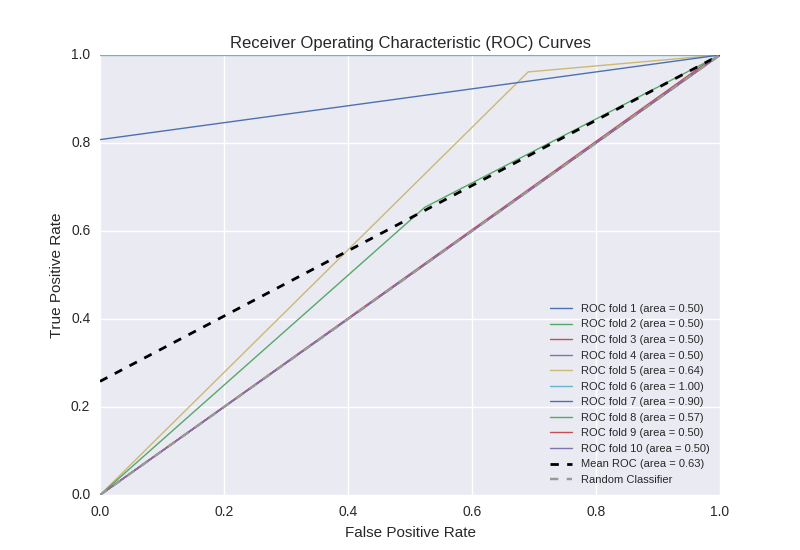
\includegraphics{./Figures/experiments/feat-eng/roc}
     }
	\caption[ROC Curves of a kNN Classifier using Standardization and the Pearson Correlation Filter]{ROC Curves of a kNN Classifier using Standardization and the Pearson Correlation Filter}
	\label{fig:feat-eng-roc-knn-pearson}
\end{figure}

\begin{figure}[H]
	\centering
	\resizebox{\textwidth}{!}{
  	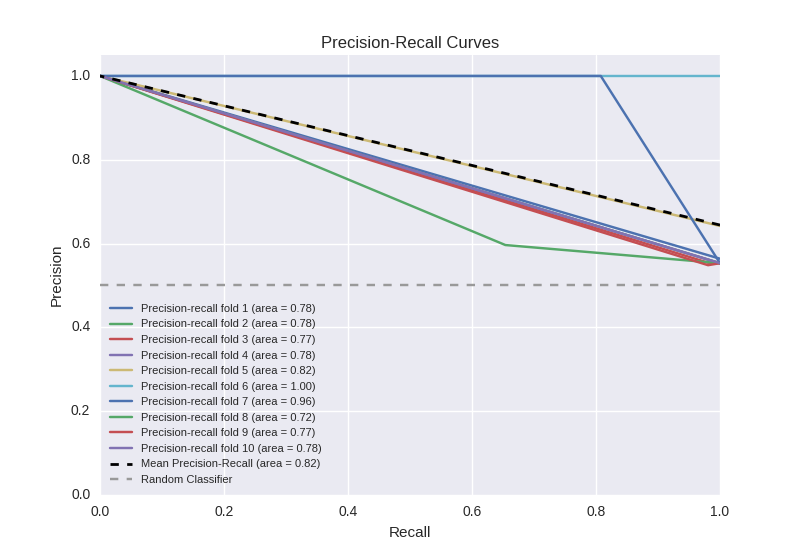
\includegraphics{./Figures/experiments/feat-eng/pr_curve}
     }
	\caption[Precision-Recall Curves of a Naive Bayes Classifier using Standardization and the Pearson Correlation Filter]{Precision-Recall Curves of a Naive Bayes Classifier using Standardization and the Pearson Correlation Filter}
	\label{fig:feat-eng-pr-nb-pearson}
\end{figure}

Although the kNN classifier achieved a score of 0.63, for small rates of false positives ($<0.4$), the number of correctly classified instances is still low. For greater false positive rates, the classifier is able to identify more more instances correctly. Regarding the precision-recall curves, the naive bayes classifier achieved a fairly good result(0.82) for the area under the curve, in some cases with areas greater than 0.90. 

In general, the obtained results provide small improvements over the baseline results. However, the baseline results compete in some cases. Depending on the requirements of the system, one may have to compromise between high precisions or high recalls.

\section{Predicting Relevance through Journalistic Criteria}
\label{sec:jcriteria}

In the previous section we focused on detecting relevance through textual features. Going further, we now describe the process of detecting relevance using an intermediate layer of classifiers. Each intermediate classifier is focused on a single task, i.e., it detects one of the following criteria: controversialness (controversial/not controversial), interestingness (interesting/not interesting), meaningfulness (meaningful/meaningless), novelty (new/old), reliability (reliable/unreliable) and scope (wide/narrow). Each one of these classifiers has as input the textual data and outputs a single prediction of a journalistic aspect. After this, the last classifier receives these journalistic predictions and outputs the final relevance prediction. The intermediate journalistic classifiers start by extracting the same textual features described in table \ref{table-features} with possible preprocessing and feature selection/reduction applied afterwards. The last classifier used these journalistic predictions as its features. Figure \ref{fig:diag-journalistic-criteria} illustrates this idea.
\begin{figure}[H]
	\centering
	\resizebox{\textwidth}{!}{
  	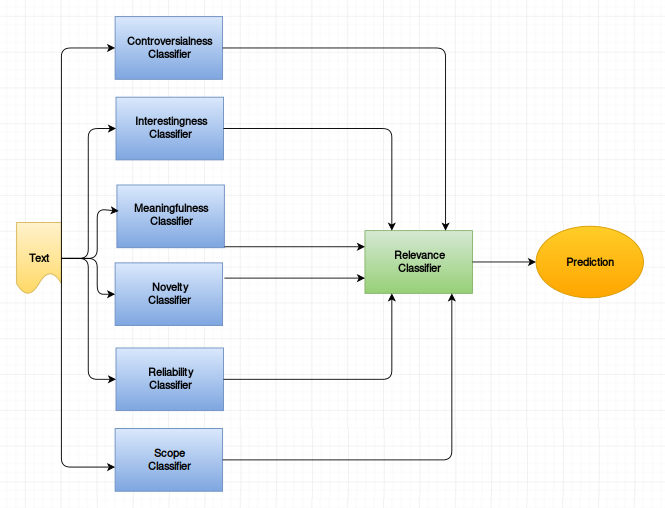
\includegraphics{./Figures/experiments/journalistic-relevance/jr}
     }
	\caption[Prediction of Relevance using Journalistic Criteria]{Prediction of Relevance using Journalistic Criteria}
	\label{fig:diag-journalistic-criteria}
\end{figure}

Table \ref{tab:theoretical-journalistic-relevance-classifiers} shows the results of training the relevance classifier, based on the 6 different, manually annotated journalistic data. The only preprocessing method applied was Standardization. For such a small feature set, we did not apply any feature selection or reduction method, since they did not provide significant improvements. We used a variation of the SVM classifier, which uses a polynomial kernel, with the intent of achieving a better decision boundary that could separate better the classes. Nevertheless, the model parameters were the same as in the baseline experiments. Table \ref{tab:theoretical-journalistic-relevance-classifiers} shows the obtained results.	
\begin{table}[H]
\centering
\small
\resizebox{\textwidth}{!}{%
\begin{tabular}{|l|c|c|c|c|c|c|}
\hline
\multicolumn{1}{|r|}{\textbf{}} & \multicolumn{6}{c|}{\textbf{Training of a Relevance Classifier based on Journalistic Criteria}} \\ \hline
\multicolumn{1}{|r|}{\textbf{Performance Metrics}} & \multirow{2}{*}{\textbf{Accuracy}} & \multirow{2}{*}{\textbf{Precision}} & \multirow{2}{*}{\textbf{Recall}} & \multirow{2}{*}{\textbf{F$_1$}} & \multirow{2}{*}{\textbf{AP}} & \multirow{2}{*}{\textbf{AUC}} \\ \cline{1-1}
\textbf{Classifier} &  &  &  &  &  &  \\ \hline
Minimum Distance Classifier & 0.80 $\pm$ 0.06 & \textbf{0.84 $\pm$ 0.07} & 0.80 $\pm$ 0.08 & 0.82 $\pm$ 0.06 & 0.87 $\pm$ 0.04 & 0.80 $\pm$ 0.06 \\ \hline
K-Nearest Neighbors& \textbf{0.82 $\pm$ 0.07} & 0.82 $\pm$ 0.07 & \textbf{0.86 $\pm$ 0.08}  & \textbf{0.84 $\pm$ 0.06} & \textbf{0.88 $\pm$ 0.04} & \textbf{0.81 $\pm$ 0.07} \\ \hline
Naive Bayes& 0.81 $\pm$ 0.06 & 0.84 $\pm$ 0.07 & 0.81 $\pm$ 0.08 & 0.82 $\pm$ 0.06 & \textbf{0.88 $\pm$ 0.04} & \textbf{0.81 $\pm$ 0.06} \\ \hline
SVM(Linear) & 0.80 $\pm$ 0.06 & 0.82 $\pm$ 0.07 & 0.84 $\pm$ 0.08 & 0.83 $\pm$ 0.06 & 0.87 $\pm$ 0.04 & 0.80 $\pm$ 0.07 \\ \hline
SVM(Polynomial Kernel) & 0.81 $\pm$ 0.06 & 0.82 $\pm$ 0.07 & \textbf{0.86 $\pm$ 0.07} & \textbf{0.84 $\pm$ 0.06} & \textbf{0.88 $\pm$ 0.04} & \textbf{0.81 $\pm$ 0.07} \\ \hline
Decision Tree& 0.79 $\pm$ 0.07 & 0.81 $\pm$ 0.07 & 0.82 $\pm$ 0.08 & 0.81 $\pm$ 0.06 & 0.87 $\pm$ 0.04 & 0.79 $\pm$ 0.07 \\ \hline
Random Forest & 0.80 $\pm$ 0.07 & 0.81 $\pm$ 0.07 & 0.84 $\pm$ 0.07 & 0.82 $\pm$ 0.06 & 0.87 $\pm$ 0.04 & 0.79 $\pm$ 0.07 \\ \hline
\end{tabular}%
}
\caption[Results on predicting Relevance based on Journalistic Criteria]{Results on predicting Relevance based on Journalistic Criteria}
\label{tab:theoretical-journalistic-relevance-classifiers}
\end{table}

From the observed results, it is clear that the SVM with the polynomial kernel and the kNN classifiers achieved the best performance, with the latter achieving a better accuracy(0.82). However, the Minimum Distance Classifier obtained the best overall precision  (0.84). For the rest of the metrics, the SVM with the polynomial kernel and the kNN achieved the overall best recall(0.86), F$_1$ score (0.84), average precision (0.88) and AUC (0.81). The naive bayes also got the best areas under the precision-recall and ROC curves. Figures \ref{fig:theoretical-journalistic-relevance-roc},\ref{fig:theoretical-journalistic-relevance-pr} shows the ROC and Precision-Recall curves. 

\begin{figure}[H]
	\centering
	\resizebox{\textwidth}{!}{
  	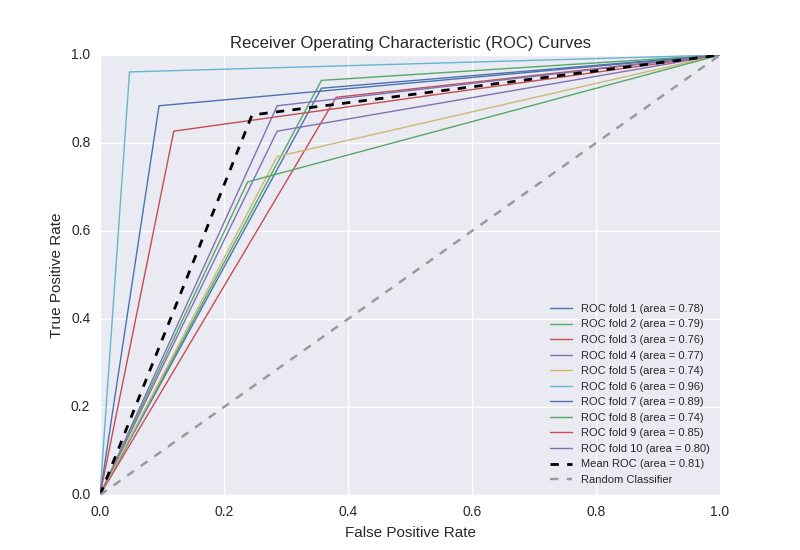
\includegraphics{./Figures/experiments/journalistic-relevance/theoretical/roc}
     }
	\caption[ROC Curves of a Journalistic Based kNN Classifier]{ROC Curves of a Journalistic Based kNN Classifier}
	\label{fig:theoretical-journalistic-relevance-roc}
\end{figure}

\begin{figure}[H]
	\centering
	\resizebox{\textwidth}{!}{
  	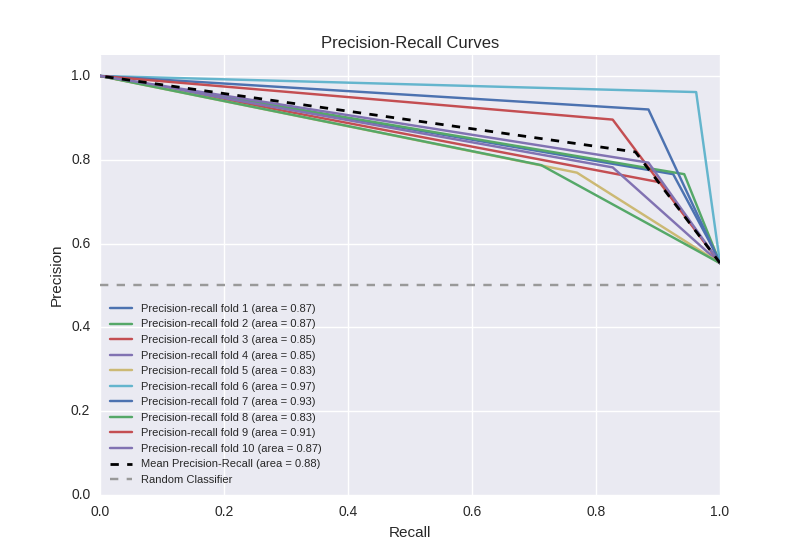
\includegraphics{./Figures/experiments/journalistic-relevance/theoretical/pr_curve}
     }
	\caption[Precision-Recall Curves of a Journalistic Based kNN Classifier]{Precision-Recall Curves of a Journalistic Based kNN Classifier}
	\label{fig:theoretical-journalistic-relevance-pr}
\end{figure}

The kNN classifier achieved a decent area under the ROC curve(0.81), showing that even for low false positive rates such as 0.2, it obtains decent true positive rates($>$ 0.7), on average. Nevertheless, in some cases, it outperformed the AUC mark of 0.85. Regarding the precision-recall curves, it achieved an area of 0.88, on a average, providing a good flexibility with the trade-offs. For high values of recall, it also obtained similar high values of precision. 

Given these results, we decided to use the kNN model as our journalistic based, relevance predictor, since it provided the best performance. As for the intermediate models, we performed 6 experiments, each one consisting of using the best found pipeline(best F$_1$ score) during the feature engineering experiments\ref{sec:feature-engineering} for each classifier. Table \ref{tab:journalistic-relevance-classifiers} details the obtained results.

\begin{table}[H]
\centering
\small
\resizebox{\textwidth}{!}{%
\begin{tabular}{|l|c|c|c|c|c|c|}
\hline
\multicolumn{1}{|r|}{\textbf{}} & \multicolumn{6}{c|}{\textbf{Relevance based on Journalistic Criteria}} \\ \hline
\multicolumn{1}{|r|}{\textbf{Performance Metrics}} & \multirow{2}{*}{\textbf{Accuracy}} & \multirow{2}{*}{\textbf{Precision}} & \multirow{2}{*}{\textbf{Recall}} & \multirow{2}{*}{\textbf{F$_1$}} & \multirow{2}{*}{\textbf{AP}} & \multirow{2}{*}{\textbf{AUC}} \\ \cline{1-1}
\textbf{Intermediate Classifiers} &  &  &  &  &  &  \\ \hline
Minimum Distance Classifiers & 0.62 $\pm$ 0.11 & 0.66 $\pm$ 0.17 & 0.89 $\pm$ 0.19 & 0.72 $\pm$ 0.08 & 0.80 $\pm$ 0.06 & 0.59 $\pm$ 0.13 \\ \hline
K-Nearest Neighbors& 0.54 $\pm$ 0.08 & 0.63 $\pm$ 0.14 & 0.57 $\pm$ 0.17 & 0.57 $\pm$ 0.08 & 0.72 $\pm$ 0.05 & 0.54 $\pm$ 0.09 \\ \hline
Naive Bayes& 0.56 $\pm$ 0.01 & 0.56 $\pm$ 0.01 & \textbf{0.97 $\pm$ 0.03} & 0.71 $\pm$ 0.01 & 0.77 $\pm$ 0.01 & 0.52 $\pm$ 0.01 \\ \hline
Linear SVMs& 0.54 $\pm$ 0.03 & 0.56 $\pm$ 0.02 & 0.89 $\pm$ 0.08 & 0.68 $\pm$ 0.03 & 0.75 $\pm$ 0.02 & 0.50 $\pm$ 0.04 \\ \hline
Decision Trees& 0.55 $\pm$ 0.05 & 0.57 $\pm$ 0.03 & 0.78 $\pm$ 0.11 & 0.65 $\pm$ 0.05 & 0.73 $\pm$ 0.03 & 0.52 $\pm$ 0.05 \\ \hline
Random Forests & \textbf{0.79 $\pm$ 0.07} & \textbf{0.80 $\pm$ 0.08} & 0.84 $\pm$ 0.07 & \textbf{0.82 $\pm$ 0.06} & \textbf{0.86 $\pm$ 0.04} & \textbf{0.78 $\pm$ 0.08} \\ \hline
\end{tabular}%
}
\caption[Results on Predicting Relevance by an Ensemble of Journalistic Classifiers]{Results on Predicting Relevance by an Ensemble of Journalistic  Classifiers}
\label{tab:journalistic-relevance-classifiers}
\end{table}

Random forests revealed to be the best option for the intermediate classifiers. They achieved the best accuracy(0.79), precision(0.80) and F$_1$(0.82) score. However, the naive bayes obtained an outstanding value for recall of 0.97. Regarding the areas below the ROC and precision-recall curves, the Random Forests also achieved the best values, obtaining 0.78 and 0.86, respectively. Figures \ref{fig:rt-journalistic-relevance-roc} and \ref{fig:rt-journalistic-relevance-pr} show the ROC and precision-recall curves, respectively.

\begin{figure}[H]
	\centering
	\resizebox{\textwidth}{!}{
  	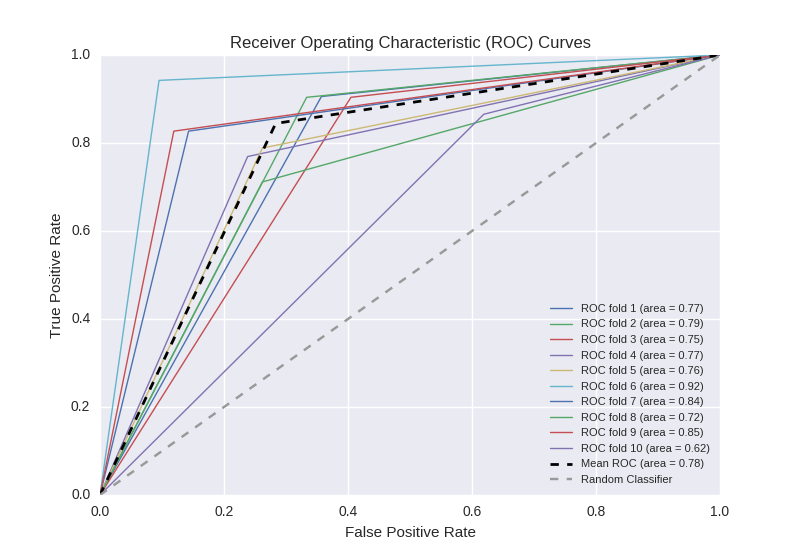
\includegraphics{./Figures/experiments/journalistic-relevance/rt/roc2}
     }
	\caption[ROC Curves of a Journalistic Based kNN Classifier, using Random Forests for the intermediate classifiers]{ROC Curves of a Journalistic Based kNN Classifier, using Random Forests for the intermediate classifiers}
	\label{fig:rt-journalistic-relevance-roc}
\end{figure}

\begin{figure}[H]
	\centering
	\resizebox{\textwidth}{!}{
  	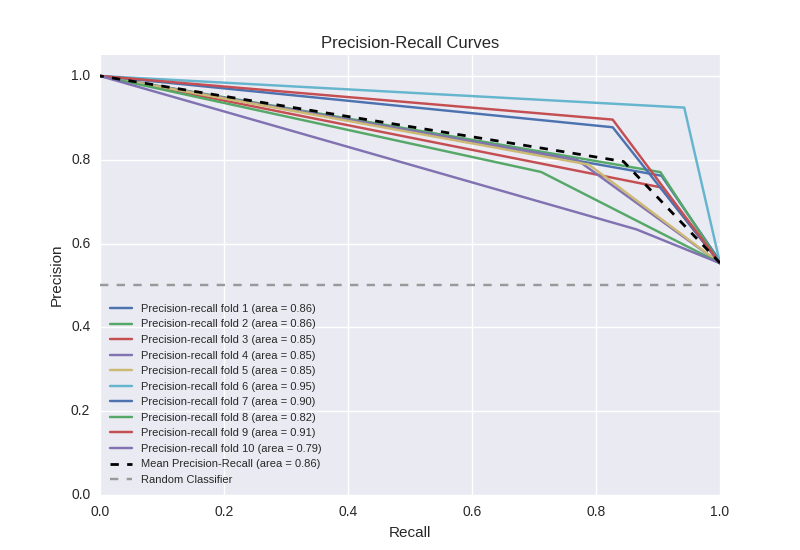
\includegraphics{./Figures/experiments/journalistic-relevance/rt/pr_curve2}
     }
	\caption[Precision-Recall Curves of a Journalistic Based kNN Classifier, using Random Forests for the intermediate classifiers]{Precision-Recall Curves of a Journalistic Based kNN Classifier, using Random Forests for the intermediate classifiers}
	\label{fig:rt-journalistic-relevance-pr}
\end{figure}

The classifier got a good mean area under the ROC curve(0.78), meaning that is able to identify and classify correctly most of the instances, even for low false positive rates. Regarding the precision-recall graph, which has a good area under the mean curve(0.85), the classifier consistently shows high values of precision, even when the recall increases.

Comparing with the initial baseline experiments, the general scenario is fairly better. There was an improvement in accuracy of 15\%, 8\% in precision and recall, 9\% in F$_1$, 6\% in average precision and 16\% in AUC.

\section{Discussion}

The obtained results suggest that using a meta classifier that makes use of an intermediate tier of the best single strong models is the preferred method. By using a Random Forest classifier to predict each one of the journalistic criteria, and a kNN classifier to detect the final relevance, it was possible to achieve the best accuracy(0.79), precision(0.80) and F$_1$ (0.82) score. In fact, seeing different aspects of the problem space (different criteria) was helpful to reduce the generalization error and variance. This method proved to be a good choice to be used in the REMINDS system. \\
Although with different goals, other system achieved similar F$_1$ performances, such as predicting spam or not spam(0.79) \citep{Irani2010TrendStuff} by using a Decision Tree (C4.5). Simiraly, Liparas et al.\citep{Liparas2014NewsClassification} achieved a F$_1$ score of 0.85 by using simple bigrams and metadata from the tweets, with a Naive Bayes, to classify web pages by topic. Fernandes et al. \citep{Fernandes2015PredictingPopularity} also used a Random Forest to predict the popularity of a web article, obtaining a F$_1$ score of 0.69.




 
% Chapter 6

\chapter{Conclusions} % Main chapter title
%\epigraph{A fancy quote.}{Me}

\label{conclusions} % For referencing the chapter elsewhere, use \ref{Chapter2} 
\lhead{Chapter 6. \emph{Conclusions}} % This is for the header on each page - perhaps a shortened title

In this work, we described the REMINDS system which will have at its core a classifier able to predict relevant information and filter out irrelevant information. More precisely, this specific work dealt with the development of a classifier for predicting the relevance of social media posts relying exclusively in linguistic features extracted from text as the main distinction from other approaches, by other partners of the REMINDS project. \\
This document started with a brief overview of the academic disciplines where this work is focused, NLP, ML \& Text Classification, describing important concepts useful to understand this work. We then made a survey of a wide range of existing techniques to solve text classification problems and also presented a technological review of existing software implementations that currently support NLP tasks and, in some cases, ML techniques. Furthermore, we described the REMINDS system global architecture, with focus on the parts that were the focus of this work.

We have shown that, using only the available pre-trained models, there is not one NLP toolkit that overperformed all the others in every scenario and pre-processing task. Nevertheless, it was an important step to decide which tools to use in the feature extraction process.

We have tackled the problem of identifying social network messages as relevant or not, from a journalistic point of view, and relying only on linguistic features. Based on a dataset of social network messages annotated by volunteer contributors, the best relevance classification model learned achieved a $F_1$-score of 0.82. This model relied on a set of intermediate classifiers using the Random Forest model, using linguistic features extracted from the textual data, with the end model based on a k-Nearest Neighbors classifier. The presented results are higher than those obtained using single feature sets with no preprocessing or feature selection/reduction applied, which highlights the importance of these additional steps.

Regarding future work, several alternatives could be explored and potentially improve the results. Starting with the feature extracting process, there are other NLP tasks that could be explored, such as: Information extraction which extracts structured knowledge like facts, events or relationships; relation extraction which identifies relationships between entities; dependency parsing which is useful to understand textual relations, such as who did what, when, where and how which could also have been used as features. On the other hand, different combinations of feature selection/reduction methods and learning models as well, could be explored. Moreover, the resulting system can be integrated with the alternative approaches, based on different features, in a larger relevance mining platform, namely the REMINDS system. 
 

%----------------------------------------------------------------------------------------
%	THESIS CONTENT - APPENDICES
%----------------------------------------------------------------------------------------

\addtocontents{toc}{\vspace{2em}} % Add a gap in the Contents, for aesthetics

\appendix % Cue to tell LaTeX that the following 'chapters' are Appendices

% Include the appendices of the thesis as separate files from the Appendices folder
% Uncomment the lines as you write the Appendices

%% Appendix A
\chapter{Potential Conferences} % Main appendix title

\label{AppendixA} % Change X to a consecutive letter; for referencing this appendix elsewhere, use \ref{AppendixX}

\lhead{Appendix A. \emph{Potential Conferences}} % Change X to a consecutive letter; this is for the header on each page - perhaps a shortened title

The scientific paper may be published in available conferences where the submission deadlines are in accordance with the working plan for the second stage of this work. The following list shows some potential candidates:
\begin{itemize}
	\item \textbf{Association for Computational Linguistics \href{http://acl2016.org}{(ACL)}} - The ACL conference will be held from August 7 to 12, 2016 in Berlin, Germany. Important dates are February 29, 2016 for short papers submissions and March 18, 2016 for long papers submissions.

	\item \textbf{European Conference on Machine Learning and Principles and Practice of Knowledge Discovery \href{http://www.ecmlpkdd2016.org}{(ECML-PKDD)}} - The ECML-PKDD conference will be held from September 19 to 23, 2016 in Riva del Garda, Italy. Important dates are April 1, 2016 for abstract submissions and April 4, 2016 for papers submissions.

    \item \textbf{European Conference on Artificial Intelligence \href{http://www.ecai2016.org}{(ECAI)}} - The ECAI conference will be held from August 29 to September 2, 2016 in The Hague, The Netherlands. An important date is April 15, 2016 for papers submissions.
    
   % \item \textbf{Workshop on Language Technologies and Applications \href{https://fedcsis.org/2016/lta}{(LTA)}} - The LTA workshop will be held from September 11 to 14, 2016 in Gdansk, Poland. An important date is April 18, 2016 for papers submissions.
    
    \item \textbf{Conference on Computational Natural Language Learning \href{http://www.conll.org/cfp-2016}{(CoNLL)}} - The CoNLL conference will be held from August 11 to 12, 2016 in Berlin, Germany. An important date is May 6, 2016 for papers submissions.
    
    \item \textbf{Conference on Intelligent Text Processing and Computational Linguistics \href{http://www.cicling.org/2016}{(CICLing)}} - The CICLing conference will be held from April 3 to 9, 2016 in Konya, Turkey. Important dates are yet to be announced.
    
    \item \textbf{Conference on Computational Linguistics \href{http://coling2016.anlp.jp}{(COLING)}} - The COLING conference will be held from December 11 to 16, 2016 in Osaka, Japan. An important date is July 15, 2016 for papers submissions.
    
\end{itemize}
%



\addtocontents{toc}{\vspace{2em}} % Add a gap in the Contents, for aesthetics

\backmatter

%----------------------------------------------------------------------------------------
%	BIBLIOGRAPHY
%----------------------------------------------------------------------------------------

\label{Bibliography}

\lhead{\emph{Bibliography}} % Change the page header to say "Bibliography"

%\bibliographystyle{amsplain} % Use the "unsrtnat" BibTeX style for formatting the Bibliography

\bibliographystyle{unsrtnat} % Use the "unsrtnat" BibTeX style for formatting the Bibliography

\bibliography{Bibliography} % The references (bibliography) information are stored in the file named "Bibliography.bib"



\end{document}